\documentclass{article}
\usepackage[a4paper,margin=1in]{geometry}

\usepackage{amsmath, amsthm, amssymb}
\usepackage{mathrsfs}
\usepackage{enumitem}
\usepackage{fancyhdr}
\usepackage{mathtools}
\usepackage{bm}
\usepackage{float}
\usepackage{graphicx}

\usepackage{tikz}
\usetikzlibrary{decorations.markings, decorations.pathreplacing, arrows.meta, positioning, shapes.geometric, trees, backgrounds, fit, calc}

\usepackage{hyperref}
\usepackage{cleveref}
\usepackage[numbers]{natbib} 

\hypersetup{
    colorlinks=true,
    citecolor=blue,
    linkcolor=blue,
    urlcolor=blue
}

\usepackage{accents}

% Allow modest interword flexibility before TeX resorts to overfull lines.
\setlength{\emergencystretch}{3em}

%% ── Theorem environments ──
%% plain style: bold label, italic body — for main results
\theoremstyle{plain}
\newtheorem{theorem}{Theorem}[section]
\newtheorem{lemma}[theorem]{Lemma}
\newtheorem{proposition}[theorem]{Proposition}
\newtheorem{corollary}[theorem]{Corollary}
\newtheorem{algorithm}[theorem]{Algorithm}


%% definition style: bold label, roman body 
\theoremstyle{definition}
\newtheorem{assumption}{Assumption}[section]
\newtheorem{definition}[theorem]{Definition}
\newtheorem{notation}[theorem]{Notation}
\theoremstyle{remark}
\newtheorem{remark}[theorem]{Remark}

%% ── Number systems ──
\newcommand{\R}{\mathbb{R}}
\newcommand{\Nbb}{\mathbb{N}}
\newcommand{\Pbb}{\mathbb{P}}
\newcommand{\Ebb}{\mathbb{E}}

%% ── Linear algebra ──
\newcommand{\Id}{\mathrm{Id}}
\newcommand{\Var}{\mathrm{Var}}
\newcommand{\Cov}{\mathrm{Cov}}
\DeclareMathOperator{\sign}{sign}
\DeclareMathOperator{\diag}{diag}
\DeclareMathOperator{\tr}{tr}

%% ── Miscellaneous ──
\newcommand{\1}{\mathbf{1}}   % indicator: \1\{event\}
\newcommand{\independent}{\perp \!\!\! \perp} 

%% cleveref names
%\crefname{assumption}{Assumption}{Assumptions}
%\Crefname{assumption}{Assumption}{Assumptions}




\AtBeginEnvironment{pmatrix}{\everymath{\displaystyle}}


\title{High-Dimensional Dynamics of Self-Training with Confidence Selection and Data Reuse}
\author{
    Matias Cattaneo\thanks{Department of Economics, Princeton University},
    Jason Klusowski\thanks{Department of Operations Research and Financial Engineering, Princeton University},
    Thierry Rioual\thanks{Department of Operations Research and Financial Engineering, Princeton University}
}



\begin{document}

\maketitle

\begin{abstract}
Self-training uses a predictor's own predictions as pseudo-labels
for further training. When the same observations are reused,
this feedback creates dependencies between the data, pseudo-labels,
and successive parameter updates.
We study confidence-thresholded self-training of affine classifiers
on partially labeled binary Gaussian mixtures, with pseudo-labels
refreshed after every gradient step.

Under suitable assumptions on the loss, penalty, and algorithm,
we establish three results.
We first prove convergence of the algorithm for a fixed dimension
and data realization.
In the proportional asymptotic regime, we characterize the
limiting empirical laws of parameter-coordinate trajectories
and training-score trajectories over every fixed time horizon
through two effective stochastic processes.
At last, under additional assumptions, we show that these effective 
parameter and score processes converge as the number of iterations 
tends to infinity.

Numerical experiments validate our theoretical findings, and we illustrate 
the dynamics via a classification error decomposition and 
a study of the effect of class imbalance.
\end{abstract}

\tableofcontents

\section{Introduction}
\label{sec:introduction}

Unlabeled data are often abundant, whereas obtaining labels may
require costly manual annotation. Self-training addresses this issue
by using a model's predictions as pseudo-labels for unlabeled
observations, which then contribute to subsequent training
\cite{lee2013pseudolabel}.

We write $\mathbb N=\{0,1,2,\ldots\}$,
$[\![a,b]\!]=\{a,a+1,\ldots,b\}$ for integers $a\leq b$,
and $\mathscr L(X)$ for the law of a random element $X$.

Given partially labeled observations
$\mathcal D:=\{(X_i,\Delta_iY_i):i\in[\![1,n]\!]\}$, where
$X_i\in\mathbb R^d$, $Y_i\in\{-1,+1\}$, and
$\Delta_i\in\{0,1\}$ indicates whether the label is observed,
we study a self-training algorithm that produces affine classifiers
of the form
\begin{equation}
    f_\theta(x)
    :=
    \operatorname{sign}\left(
        b+\frac{x^\top w}{\sqrt d}
    \right),
    \qquad
    \theta=(b,w)\in\mathbb R\times\mathbb R^d,
    \label{eq:def-classifier}
\end{equation}
with $\operatorname{sign}(0)=+1$.
Let
$I_{\mathcal U}:=\{i\in[\![1,n]\!]:\Delta_i=0\}$
denote the indices of the unlabeled observations.
At each iteration $t$, the current classifier assigns to each
$j\in I_{\mathcal U}$ a training score and a pseudo-label
\[
    r_j^t
    :=
    b^t+\frac{X_j^\top w^t}{\sqrt d},
    \qquad
    \widehat Y_j^t
    :=
    \operatorname{sign}(r_j^t).
\]
Given confidence thresholds $\kappa_-<0<\kappa_+$,
only observations with sufficiently confident scores are retained,
forming the pseudo-labeled dataset
\begin{align}
    \mathcal P_t
    :=
    \bigl\{(X_j,\widehat Y_j^t):j\in I_t\bigr\},
    \qquad
    I_t
    :=
    \left\{
        j\in I_{\mathcal U}:
        r_j^t\le\kappa_-
        \ \text{or}\
        r_j^t\ge\kappa_+
    \right\}.
    \label{eq:pl-dataset}
\end{align}
The model is then updated by taking one gradient step,
\begin{align}
    \theta^{t+1}
    :=
    \theta^t
    -
    \eta P_d
    \nabla_\theta L(\theta^t;\mathcal D_L,\mathcal P_t), 
    \label{eq:pl-gd-step}
\end{align}
where
$\mathcal D_L:=\{(X_i,Y_i):\Delta_i=1\}$
is the labeled dataset, $L$ is the surrogate objective
specified in \eqref{eq:ST-objective}, and $P_d$ is a
preconditioning matrix. Its pseudo-labeled contribution is
weighted by $\pi$ and normalized by the full unlabeled count $M$.
This procedure is repeated, with the same labeled and unlabeled
observations reused throughout training.

Unlike ordinary empirical risk minimization, the training objective
changes at each iteration, as the pseudo-labels and selected
observations depend on the current classifier. These adaptive
changes introduce discontinuities into the update rule and
nonconvexity into the underlying optimization problem.
The statistical analysis presents additional difficulties.
Because the same random observations are reused throughout
training, successive parameter updates are coupled through
their dependence on the data and previous iterates.
Furthermore, we are interested in understanding these dynamics
in the high-dimensional regime, where many tools from classical
asymptotic statistics are no longer applicable.

These considerations raise two natural questions:
\begin{itemize}
    \item Does the self-training algorithm converge, and what
    can be said about its limiting point?
    \item Can the dynamics of the parameter iterates and their
    statistical performance be characterized precisely in
    high dimensions?
\end{itemize}

\subsection{Contributions}

We address these questions by establishing convergence of the
self-training algorithm and deriving an asymptotically exact
characterization of its finite-time dynamics under a Gaussian-mixture
model in the high-dimensional regime.
The precise setting and assumptions are presented in
Section~\ref{sec:setting}. Our main contributions are threefold:

\begin{enumerate}
    \item \emph{Finite-dimensional convergence.}
    Under suitable assumptions, we prove that the self-training
    parameters converge for a fixed dataset, with an eventual
    geometric rate of convergence. We further characterize the
    limiting point in terms of the final pseudo-labeling and
    selection configuration.

    \item \emph{Asymptotically exact dynamics.}
    In the proportional asymptotic regime, we
    characterize the limiting empirical laws of
    parameter-coordinate trajectories and sample-score
    trajectories over every fixed time horizon through
    two effective stochastic processes.

    \item \emph{Long-time convergence.}
    Under additional assumptions, we establish convergence of
    the effective parameter and score processes as the number
    of iterations tends to infinity, with the high-dimensional
    limit taken first. For a representative unlabeled observation,
    the selection state and the assigned label when selected
    eventually stabilize almost surely.
\end{enumerate}

Our results provide foundations for further analysis of
self-training algorithms.
Section~\ref{sec:numerical} takes initial steps toward
understanding improvements in generalization and the effects
of class imbalance.
A comprehensive quantitative analysis of these mechanisms,
and of the trade-off between pseudo-label reliability and
the fraction of selected observations, remains open.

Section~\ref{sec:related-work} reviews self-training,
self-distillation, adaptive training procedures, and
high-dimensional dynamics.
Section~\ref{sec:setting} specifies the model and algorithm.
Section~\ref{sec:main-result} presents the finite-dimensional,
mean-field, and long-time results, proved respectively in
Appendices~\ref{sec:proof-finite-dim},
\ref{sec:proof-mean-field}, and \ref{sec:proof-long-time}.
Section~\ref{sec:numerical} presents numerical validation and
statistical interpretation, with proofs in
Appendix~\ref{sec:proof-numerical}.
Appendix~\ref{sec:math-prelim} collects mathematical preliminaries 
that might be useful to the reader.

\section{Related Work}
\label{sec:related-work}

\subsection{Self-Training}
\label{subsec:st}

Despite its popularity, self-training does not always improve
predictive performance, which can depend on initialization,
hyperparameters, and the unlabeled data
\cite{oliver2018realistic,su2021realistic}.
While self-training has been studied extensively in empirical work
\cite{amini2025survey,vanengelen2020survey,yang2023survey,kage2026review},
its theoretical understanding remains limited.
To address the challenges discussed in Section~\ref{sec:introduction},
existing theoretical analyses have considered various
simplifications of the self-training procedure.

For instance, Wei et al.~\cite{wei2021theoretical} establish accuracy guarantees
for fixed pseudo-labelers with consistency regularization.
Oymak and Gulcu~\cite{oymak2020} analyze confidence-thresholded
averaging estimators, using fresh batches for iterative characterization.
Frei et al.~\cite{frei2022selftraining} establish accuracy guarantees
for gradient-based self-training with fresh batches.
Other theoretical analyses investigate iterative
self-training under different structural assumptions.
Chen et al.~\cite{chen2020selftraining} study gradient-based
self-training under domain shift.
He et al.~\cite{he2022information} derive information-theoretic
generalization expressions.
Zhang et al.~\cite{zhang2022unlabeled} establish convergence and
generalization guarantees for neural-network regression.
Li et al.~\cite{li2025fixmatch} analyze FixMatch-like
gradient updates with adaptive pseudo-labels on fixed datasets.
Heidarizadeh et al.~\cite{heidarizadeh2026confidence} derive
generalization bounds under gradual domain shift.
Closer to our proportional-asymptotic setting,
Takahashi~\cite{takahashi2026role} derives sharp predictions
for linear classifiers on Gaussian mixtures, using fresh batches
and stagewise minimization.
Takanami et al.~\cite{takanami2025effect} analyze repeated-data
self-distillation with temperature-controlled soft pseudo-labels,
including hard pseudo-labels as a limiting case, and stagewise
minimization, but without confidence selection.
Both works rely on non-rigorous replica calculations from physics.

Our analysis combines gradient updates, confidence selection,
and repeated data reuse within a single rigorous framework.
The algorithm incorporates pseudo-labels refreshed at each
gradient step~\cite{lee2013pseudolabel}, hard pseudo-labeling
and confidence-based selection~\cite{sohn2020fixmatch},
and allows asymmetric confidence thresholds for the two
predicted classes, motivated by class-dependent selection
strategies~\cite{zhang2021flexmatch}.
To the best of our knowledge, no previous analysis establishes
rigorous, asymptotically exact empirical trajectory laws for
both parameter coordinates and training scores with this
combination of features in the proportional regime.

\subsection{Self-Distillation}
\label{subsec:sd}

A related procedure is self-distillation, where a student learns
from the predictions of a previously trained teacher, possibly
alongside the original labels.
While the two procedures are closely related, their objectives
typically differ.
Self-distillation aims to improve an existing estimator through
regularization, denoising, or feature transfer, whereas
semi-supervised self-training seeks to exploit the structure
of unlabeled data to improve a classifier trained on limited
labeled observations.

Self-distillation has a substantial theoretical literature,
particularly in regression, where explicit expressions or
tractable characterizations of successive minimizers allow
precise analysis through spectral and random matrix methods.
Mobahi et al.~\cite{mobahi2020selfdistillation} characterize
regularization through spectral filtering.
Das and Sanghavi~\cite{das2023understanding} study the effects
of regularization and label noise, while Pareek et
al.~\cite{pareek2024understanding} establish improvements
from repeated distillation.
Wu et al.~\cite{wu2026selftraininghelpshurtsdenoising} derive
high-dimensional risk recursions revealing a trade-off between
denoising and signal forgetting.
Further precise results are obtained by Dang et al.~\cite{dang2026}
and Lecoiu et al.~\cite{lecoiu2026}.
Classification has also been studied.
Das and Sanghavi~\cite{das2023understanding} establish accuracy
improvements for logistic classifiers under restrictive feature
assumptions, while Takanami et al.~\cite{takanami2025effect}
derive replica predictions for repeated-data Gaussian-mixture
classification.
Javanmard et al.~\cite{javanmard2025selfboost} derive 
AMP-based characterizations of iterative retraining with reused data, 
combining model predictions with noisy observed labels in 
Gaussian-mixture and generalized-linear models.

These works primarily analyze successive fitted predictors,
often exploiting special structure to obtain explicit statistical
characterizations.
Our setting instead studies the optimization dynamics themselves,
where confidence selection of hard pseudo-labels creates
discontinuities at the selection thresholds, and repeated
data reuse couples successive gradient updates.
These features prevent the direct spectral reductions available
in much of the self-distillation literature.

\subsection{Adaptive Training Procedures}
\label{subsec:adapt}

Our work relates to optimization procedures in which the
training objective depends on the current model.
In performative prediction, model deployment changes the
distribution of subsequent observations.
Perdomo et al.~\cite{perdomo2020performative} and
Mendler-D\"unner et al.~\cite{mendlerdunner2020stochastic}
establish convergence guarantees for repeated risk
minimization and stochastic optimization, with further
results on decision-dependent distributions
in~\cite{drusvyatskiy2023stochastic,cutler2024stochastic}.
Related work on adaptive sample selection includes
iterative trimmed-loss minimization, for which
Shen and Sanghavi~\cite{shen2019trimmed} establish
convergence and statistical guarantees, and
Aravkin and Davis~\cite{aravkin2020trimmed} derive
optimization complexity guarantees.
Nonconvex optimization also arises in semi-supervised
support vector machines, where several methods have been
developed~\cite{chapelle2008optimization,
collobert2006large, piccialli2024}.

Our finite-dimensional convergence analysis is related
to these approaches to adaptive and nonconvex optimization, but
we derive empirical trajectory laws for parameter coordinates
and training scores in the proportional high-dimensional regime,
accounting for adaptive hard pseudo-labels, confidence
selection, and repeated data reuse.


\subsection{High-Dimensional Dynamics}
\label{subsec:high-dim-dynamics}

The high-dimensional behavior of first-order optimization
algorithms has been studied through several approaches.
Paquette et al.~\cite{paquette2022} derive risk trajectories
for stochastic gradient descent on high-dimensional quadratic
objectives, while Ben Arous et
al.~\cite{arous2021online,arous2023highdimensional}
study scaling limits and effective dynamics of online
stochastic gradient descent in nonconvex inference problems.
Another approach originates from statistical physics, where
mean-field methods simplify systems with many interacting
degrees of freedom by describing their collective behavior
through macroscopic observables.
This viewpoint has motivated a substantial literature on
statistical inference and learning
\cite{mezard2009information,zdeborova2016statistical}.
Dynamical mean-field theory (DMFT) extends this approach
to evolving systems, describing limiting trajectories
through representative \emph{effective stochastic processes}.
When the same random data are repeatedly reused, these
processes generally involve memory terms and temporally
correlated Gaussian fluctuations.

Rigorous DMFT descriptions of first-order methods have
been established by Celentano, Cheng, and
Montanari~\cite{celentano2026highdimensionalasymptoticsordermethods}
through a reduction to approximate message passing (AMP),
and by Gerbelot et al.~\cite{gerbelot2024rigorous}
through iterative Gaussian conditioning.
Mignacco et al.~\cite{Mignacco_2021} derive dynamical
mean-field equations for gradient-based classification
of Gaussian mixtures, providing a related statistical-physics
analysis without confidence selection.
AMP is closely related to DMFT.
Its key feature is the Onsager correction, which compensates
for correlations generated by repeated matrix use,
leading to a simpler effective description through
\emph{state evolution}: deterministic recursions tracking
the limiting distributions of the iterates.
For Gaussian matrices, rigorous AMP analyses use Gaussian
conditioning, as in Bolthausen~\cite{bolthausen2009}
and Bayati and Montanari~\cite{bayati2011dynamics};
see also~\cite{feng2022unifying}.
Ranasinghe et al.~\cite{ranasinghe2026state} extend scalar
AMP state evolution to certain discontinuous denoisers, although applying
their results to our recursion requires an AMP reduction.
Yang's tensor programs provide another framework for
characterizing limiting coordinate laws of random-matrix
computations, including neural-network training
\cite{yang2020neuralmatrixlaws,yang2022}.
Applying these frameworks to our recursion requires accommodating 
hard confidence selection, evolving scalar parameters such as the 
intercept that shift the selection boundaries, 
and a mean-shifted Gaussian design.
Beyond finite-horizon characterization, the long-time
behavior of effective processes presents additional challenges.
Celentano et
al.~\cite{celentano2026highdimensionalasymptoticsordermethods}
derive fixed-point equations under exponential convergence
conditions, while Chen and
Shen~\cite{chen2025learningsingleindexmodel}
establish long-time DMFT convergence under suitable local
curvature assumptions.
Fan et al.~\cite{fan2025dynamicalmeanfieldanalysisadaptivepropagation,
fan2025dynamicalmeanfieldanalysisadaptivereplica}
study finite-horizon and equilibrium behavior of adaptive
Langevin dynamics under additional assumptions.

These frameworks provide general tools for analyzing
high-dimensional dynamics.
For our recursion, a direct application requires additional
arguments for discontinuous confidence selection combined
with evolving scalar shifts and data reuse.
We develop a self-contained Gaussian conditioning
argument tailored to our recursion, constructing the Gaussian
innovations, projections, and limiting effective processes.
We further establish long-time convergence of these processes.

\section{Setting}
\label{sec:setting}

Unless otherwise specified, finite-dimensional quantities depend
on $d$, with this dependence suppressed when unambiguous.
We write $\mathscr P_2(E)$ for the Borel probability measures on
$E\subseteq\mathbb R^k$ with finite second moment, $W_2$ for the
$2$-Wasserstein distance, and $\delta_x$ for the Dirac measure at $x$.
See Appendix~\ref{subsec:wasserstein} for further details on Wasserstein spaces.

\subsection{Model}

\begin{definition}[Binary Gaussian Mixture Model]
\label{def:gaussian-mixture-model}
Let $d\ge1$ be the dimension, $n\ge1$ the sample size,
$\mu\in\mathbb R^d$ the signal vector, and
$Y\in\{-1,+1\}^n$, $\Delta\in\{0,1\}^n$
the vectors of true labels and supervision indicators,
respectively. These quantities are deterministic.
Fix a noise scale $\sigma>0$. The feature vectors are
generated according to
\begin{equation}
    X_i
    =
    \frac{Y_i\mu}{\sqrt d}+\sigma U_i,
    \qquad
    U_i\stackrel{\mathrm{i.i.d.}}{\sim}
    \mathcal N(0_d,I_d),
    \qquad i\in[\![1,n]\!].
    \label{eq:gaussian-mixture-model}
\end{equation}
Thus, the observations are independent Gaussian vectors,
with class memberships determined by the fixed labels.
Only labels with $\Delta_i=1$ are observed, giving the
partially labeled dataset
\[
    \mathcal D
    :=
    \{(X_i,\Delta_iY_i):i\in[\![1,n]\!]\}.
\]
\end{definition}
For later use, define the labeled and unlabeled index sets
\[
    I_{\mathcal L}
    :=
    \{i\in[\![1,n]\!]:\Delta_i=1\},
    \qquad
    I_{\mathcal U}
    :=
    \{i\in[\![1,n]\!]:\Delta_i=0\},
\]
with cardinalities
$N:=\#I_{\mathcal L}$ and $M:=\#I_{\mathcal U}$.
Write $\delta := n / d$ for the sample-to-dimension ratio, $\rho := N/n$ for the labeled proportion,
and $p=\#\{i: Y_i=+1\}/n$ for the positive-class proportion.
We also define the empirical signal-coordinate and
sample-type laws
\begin{equation}
    \nu_\mu
    :=
    \frac1d\sum_{k=1}^d\delta_{\mu_k},
    \qquad
    \nu_{(Y,\Delta)}
    :=
    \frac1n\sum_{i=1}^n\delta_{(Y_i,\Delta_i)}.
    \label{eq:empirical-environment-laws}
\end{equation}
General empirical-measure notation is introduced in
Section~\ref{subsec:empirical-measures}.
Classical asymptotic statistics typically considers a fixed
parameter dimension as the sample size grows.
When the dimension is comparable to the sample size,
classical approximations may fail~\cite{sur2019modern}.
Nevertheless, aggregate quantities can exhibit predictable
limiting behavior even when individual coordinates remain random.
This motivates the \emph{proportional asymptotic regime}, in which
\[
    n,d\longrightarrow\infty,
    \qquad
    \frac nd\longrightarrow\bar\delta\in(0,\infty).
\]
More precisely, the proportional asymptotic regime considers
a sequence of statistical models indexed by the dimension $d$,
rather than a single fixed-dimensional model.
The sample size $n=n(d)$, signal vector $\mu=\mu(d)$,
labels $Y=Y(d)$, and supervision indicators
$\Delta=\Delta(d)$ all depend on $d$.
By imposing suitable conditions on their asymptotic behavior,
we can obtain precise limiting descriptions as $d\to\infty$.
We suppress this dependence on $d$ in the notation and
formalize these conditions in the following assumption.
\begin{assumption}[Asymptotic Regime]
\label{assumption:asymptotic-regime}
As $d\to\infty$, assume that
\begin{equation}
    \delta\longrightarrow\bar\delta,
    \qquad
    \nu_\mu\xrightarrow{W_2}\bar\nu_\mu,
    \qquad
    \nu_{(Y,\Delta)}
    \xrightarrow{W_2}\bar\nu_{(Y,\Delta)},
    \label{eq:finite-dim-limits}
\end{equation}
with $\bar \delta\in(0,\infty)$.
In particular, the positive-class and labeled proportions
converge:
\begin{equation}
    p\longrightarrow\bar p,
    \qquad
    \rho\longrightarrow\bar\rho.
    \label{eq:finite-dim-limits-2}
\end{equation}
We assume $\bar p,\bar\rho\in(0,1)$.
Consequently, $N,M\to\infty$, and both are positive
for all sufficiently large $d$.
\end{assumption}
In what follows, we restrict attention to dimensions
for which $N,M\ge1$.

\subsection{Self-Training Algorithm}

We now formalize the self-training algorithm introduced in
Section~\ref{sec:introduction}.
For $\theta=(b,w)\in\mathbb R^{d+1}$, define the
augmented feature vector and score function
\[
    \breve X_i
    :=
    \begin{bmatrix}
        1\\
        X_i/\sqrt d
    \end{bmatrix},
    \qquad
    r_i(\theta)
    :=
    \breve X_i^\top\theta
    =
    b+\frac{X_i^\top w}{\sqrt d},
    \qquad
    i \in [\![1,n]\!].
\]
Let $\ell:\{-1,+1\}\times\mathbb R\to\mathbb R$
be a differentiable loss function,
$j:\mathbb R\to\mathbb R$ a differentiable penalty function, and let $\kappa := (\kappa_-,\kappa_+)$ be selection thresholds, with $\kappa_- < 0 < \kappa_+$.
We write
\[
    \ell'(y,r)
    :=
    \frac{\partial}{\partial r}\ell(y,r),
    \qquad
    J(w):=\sum_{k=1}^d j(w_k),
    \qquad 
    S_\kappa(r) := \mathbf1_{ \{ r \le \kappa_-\} } + \mathbf1_{ \{ r \ge \kappa_+\} }.
\]
For a teacher parameter $\vartheta \in \mathbb{R}^{d+1}$ and $j \in I_{\mathcal U}$, the associated pseudo-label is $\widehat Y_j(\vartheta):=\operatorname{sign}(r_j(\vartheta))$, and
the confidence-selection step in \eqref{eq:pl-dataset}
can be expressed through the selection indicator $S_j(\vartheta) := S_\kappa(r_j(\vartheta))$. 
The indicator $S_j(\vartheta)$ ensures that unselected
observations do not contribute to the training objective.
We use the convention $\operatorname{sign}(0)=+1$.

Fix dimension-independent coefficients $\lambda,\pi\ge0$.
The self-training objective, with teacher parameter
$\vartheta$ and student parameter $\theta$, is
\begin{align}
    L_{\mathrm{ST}}(\theta;\vartheta)
    :=
    &\frac1N\sum_{i\in I_{\mathcal L}}
        \ell\bigl(Y_i,r_i(\theta)\bigr)
    +
    \frac{\pi}{M}\sum_{j\in I_{\mathcal U}}
        S_j(\vartheta)
        \ell\bigl(\widehat Y_j(\vartheta),r_j(\theta)\bigr)
    +
    \frac{\lambda}{d}J(w).
    \label{eq:ST-objective}
\end{align}
At iteration $t$, this is the objective
$L(\theta;\mathcal D_L,\mathcal P_t)$ introduced in
\eqref{eq:pl-gd-step}, with
$\vartheta=\theta^t$ held fixed.

We study the procedure in which the teacher is refreshed
after every gradient step. Starting from
$\theta^0=(b^{\mathrm{init}},w^{\mathrm{init}})$,
the iteration is
\begin{equation}
    \theta^{t+1}
    :=
    \theta^t-\eta P_d
    \nabla_1L_{\mathrm{ST}}(\theta^t;\theta^t),
    \qquad t\ge0,
    \label{eq:ST-recursion}
\end{equation}
where $\nabla_1$ denotes differentiation with respect
to the student parameter only, $\eta>0$ is the step size,
and
\[
    P_d
    :=
    \begin{bmatrix}
        1 & 0_d^\top\\
        0_d & dI_d
    \end{bmatrix}
    \in\mathbb R^{(d+1)\times(d+1)}.
\]
This preconditioning gives a nontrivial scaling of the
parameter updates in the proportional regime.
The explicit updates are summarized below.

\begin{algorithm}[Self-Training]
\label{alg:self-training}
Fix $d\ge1$ with $N,M\ge1$.
\begin{itemize}[wide]
    \item \textbf{Input:}
    Dataset $\mathcal D$, initialization
    $(b^{\mathrm{init}},w^{\mathrm{init}})$,
    number of iterations $T\in\mathbb N$,
    and hyperparameters
    $\eta$, $\lambda,\pi\ge0$ and $\kappa_-<0<\kappa_+$.

    \item \textbf{Initialization:}
    Set
    \[
        b^0:=b^{\mathrm{init}},
        \qquad
        w^0:=w^{\mathrm{init}}.
    \]

    \item \textbf{Iterations:}
    For $t=0,\ldots,T-1$:

    Compute the scores, and the pseudo-labels and selection indicators:
    \begin{align*}
        &r_i^t
        :=
        b^t+\frac{X_i^\top w^t}{\sqrt d},
         & &i\in[\![1,n]\!], \\
        \widehat Y_j^t :=\operatorname{sign}(r_j^t), &
        \qquad
        S_j^t
        :=
        \mathbf 1_{\{r_j^t\le\kappa_-\}}
        +
        \mathbf 1_{\{r_j^t\ge\kappa_+\}}
        , &&j\in I_{\mathcal U}
        .
    \end{align*}
    
    Update the intercept and weights:
    \begin{align*}
        b^{t+1}
        &:=
        b^t-\eta\Biggl[
            \frac1N\sum_{i\in I_{\mathcal L}}
                \ell'(Y_i,r_i^t)
            +
            \frac{\pi}{M}\sum_{j\in I_{\mathcal U}}
                S_j^t\ell'(\widehat Y_j^t,r_j^t)
        \Biggr],\\
        w^{t+1}
        &:=
        w^t-\eta d\Biggl[
            \frac1N\sum_{i\in I_{\mathcal L}}
                \ell'(Y_i,r_i^t)\frac{X_i}{\sqrt d}
            +
            \frac{\pi}{M}\sum_{j\in I_{\mathcal U}}
                S_j^t\ell'(\widehat Y_j^t,r_j^t)
                \frac{X_j}{\sqrt d}
            +
            \frac{\lambda}{d}\nabla J(w^t)
        \Biggr].
    \end{align*}

    \item \textbf{Output:}
    The classifier $f_{\theta^T}$,
    where $\theta^T=(b^T,w^T)$.
\end{itemize}
\end{algorithm}

The assumptions required for our main results differ and
are introduced alongside the corresponding theorems.
Nevertheless, all conditions imposed on the loss and penalty
are satisfied by the logistic loss and ridge penalty
\begin{equation}
    \ell(y,r):=\log(1+e^{-yr}),
    \qquad
    j(u):=\frac{u^2}{2}.
    \label{eq:logistic-loss-ridge-penalty}
\end{equation}


\section{Main Results}
\label{sec:main-result}

We distinguish three limiting regimes. First, we let the number of iterations tend to infinity with the dimension and training sample fixed, studying convergence of the self-training algorithm on a given dataset. Second, we let the dimension and sample size grow proportionally while keeping the iteration horizon fixed, obtaining an effective description of the training trajectory. Third, we study the long-time behavior of this limiting trajectory, establishing convergence and stabilization after the high-dimensional limit has been taken. 

\subsection{Convergence of the finite-dimensional dynamics}
\label{subsec:finite-dim}

Fix $d\geq1$ and a labeled and unlabeled sample with
$N,M\geq1$, and assume that the labeled sample contains
both classes. The feature vectors are arbitrary and fixed.
Under the assumptions below and a suitable constant step size,
we prove that the iterates identify a pseudo-labeling
configuration in finitely many iterations and converge
at an eventual geometric rate to the minimizer of the
corresponding branch objective.

\begin{assumption}[Shape and curvature of loss and penalty]
\label{assumption:finite-dim-loss-penalty}
We assume the following:
\begin{enumerate}
    \item For each $y\in\{-1,+1\}$, the function
    $r\mapsto\ell(y,r)$ belongs to
    $C^2(\mathbb R;[0,\infty))$. There exists
    $L_\ell\in(0,\infty)$ such that
    \[
        y\ell'(y,r)<0,
        \qquad
        0<\ell''(y,r)\leq L_\ell,
        \qquad
        y\in\{-1,+1\},\quad r\in\mathbb R.
    \]

    \item The penalty $j$ belongs to
    $C^2(\mathbb R;[0,\infty))$ and is coercive.
    There exists $L_j\in(0,\infty)$ such that
    \[
        0<j''(u)\leq L_j,
        \qquad u\in\mathbb R.
    \]
\end{enumerate}
\end{assumption}

\subsubsection{Potential formulation}

Write
\[
    L_{\mathcal L}(\theta)
    :=
    \frac1N\sum_{i\in I_{\mathcal L}}
        \ell(Y_i,r_i(\theta)),
    \qquad
    G(\theta)
    :=
    \nabla_1L_{\mathrm{ST}}(\theta;\theta).
\]
Here the derivative is taken with the teacher parameter held fixed.
The recursion therefore becomes
\begin{equation}
    \theta^{t+1}
    =
    \theta^t-\eta P_dG(\theta^t),
    \qquad t\geq0.
    \label{eq:ST-recursion-G}
\end{equation}
Although $G$ is discontinuous at the selection thresholds,
it agrees almost everywhere with the gradient of a continuous
potential $V$. The selection convention specifies the update
at points where this potential may fail to be differentiable.

\begin{proposition}[Self-training potential]
\label{prop:ST-potential}
Under Assumption~\ref{assumption:finite-dim-loss-penalty}, define
\[
    \psi_\kappa(r)
    :=
    \mathbf1_{\{r\leq\kappa_-\}}\ell'(-1,r)
    +\mathbf1_{\{r\geq\kappa_+\}}\ell'(+1,r),
    \qquad
    \Psi_\kappa(r)
    :=
    \int_0^r\psi_\kappa(u)\,du.
\]
Then $\Psi_\kappa$ is bounded and globally Lipschitz.
The function $V:\mathbb R^{d+1}\to\mathbb R$ defined by
\[
    V(\theta)
    :=
    L_{\mathcal L}(\theta)
    +\pi V_{\mathcal U}(\theta)
    +\frac{\lambda}{d}J(w),
    \qquad
    V_{\mathcal U}(\theta)
    :=
    \frac1M\sum_{j\in I_{\mathcal U}}
        \Psi_\kappa(r_j(\theta))
\]
is continuous and twice continuously differentiable outside
the threshold set
\[
    \mathcal S_\kappa
    :=
    \bigcup_{j\in I_{\mathcal U}}
    \left(
        \{\theta:r_j(\theta)=\kappa_-\}
        \cup
        \{\theta:r_j(\theta)=\kappa_+\}
    \right),
\]
which is a finite union of proper affine hyperplanes. For every
$\theta\notin\mathcal S_\kappa$,
\[
    \nabla V(\theta)=G(\theta).
\]
\end{proposition}

To describe the branch structure, we record the selected
pseudo-labels.
A configuration is an element of
$\{-1,0,+1\}^{I_{\mathcal U}}$.
Define the configuration map
\[
    \mathfrak C:\mathbb R^{d+1}\to\{-1,0,+1\}^{I_{\mathcal U}}, \qquad 
    \mathfrak C(\theta)
    :=
    \bigl(S_j(\theta)\hat Y_j(\theta)\bigr)_{j\in I_{\mathcal U}}.
\]
For each configuration $\mathfrak c$, define its branch by
\[
    \Theta_{\mathfrak c}
    :=
    \{\theta\in\mathbb R^{d+1}:
        \mathfrak C(\theta)=\mathfrak c\},
\]
and its smooth branch objective
$L_{\mathfrak c}:\mathbb R^{d+1}\to\mathbb R$ by
\[
    L_{\mathfrak c}(\theta)
    :=
    L_{\mathcal L}(\theta)
    +
    \frac{\pi}{M}
    \sum_{\substack{j\in I_{\mathcal U}\\\mathfrak c_j\neq0}}
        \ell(\mathfrak c_j,r_j(\theta))
    +
    \frac{\lambda}{d}J(w).
\]

\begin{proposition}[Configuration and branch formulation]
\label{prop:configuration-branch-formulation}
For each configuration $\mathfrak c$, there exists a constant
$K_{\mathfrak c}$ such that
\[
    V=L_{\mathfrak c}+K_{\mathfrak c}
        \quad\text{on}\quad\overline{\Theta_{\mathfrak c}},
    \qquad
    G=\nabla L_{\mathfrak c}
        \quad\text{on}\quad\Theta_{\mathfrak c}.
\]
Each branch is convex, possibly empty, and is described by finitely
many strict or non-strict affine inequalities.
Each nonempty branch has a polyhedral closure, and the nonempty
branches partition $\mathbb R^{d+1}$ into at most $3^M$ regions.
\end{proposition}
Consequently, the self-training recursion satisfies
\[
    \theta^{t+1}
    =
    \theta^t-\eta P_d
    \nabla L_{\mathfrak C(\theta^t)}(\theta^t),
    \qquad t\geq0,
\]
including at selection thresholds.
\begin{proposition}[Branch curvature and coercivity]
\label{prop:branch-convexity-coercivity}
Suppose Assumption~\ref{assumption:finite-dim-loss-penalty} holds.
Assume that $\lambda>0$, $\pi\geq0$, $\kappa_-<0<\kappa_+$,
and both classes occur among the labeled observations.

Then every branch objective $L_{\mathfrak c}$ has a
positive-definite Hessian on $\mathbb R^{d+1}$ and is therefore
strictly convex. Moreover, $L_{\mathfrak c}$ and the potential
$V$ are coercive:
\[
    L_{\mathfrak c}(\theta)\longrightarrow+\infty,
    \qquad
    V(\theta)\longrightarrow+\infty
    \qquad\text{as }\|\theta\|\longrightarrow\infty.
\]
Consequently, each branch objective admits a unique global minimizer,
denoted by
\[
    \theta_{\mathfrak c}^\star
    :=
    \operatorname*{argmin}_{\theta\in\mathbb R^{d+1}}
        L_{\mathfrak c}(\theta).
\]
\end{proposition}


\subsubsection{Algorithmic convergence}

To state the step-size condition, define
\begin{align}
    H_d
    &:=
    \frac{L_\ell}{N}\sum_{i\in I_{\mathcal L}}
        \breve X_i\breve X_i^\top
    +
    \frac{\pi L_\ell}{M}\sum_{j\in I_{\mathcal U}}
        \breve X_j\breve X_j^\top
    +
    \frac{\lambda L_j}{d}
    \begin{bmatrix}
        0 & 0_d^\top\\
        0_d & I_d
    \end{bmatrix}, \label{eq:hessian} \\
    \Lambda_d
    &:=
    \lambda_{\max}(P_d^{1/2}H_dP_d^{1/2})>0. \label{eq:lambda-d}
\end{align}
By Proposition~\ref{prop:branch-convexity-coercivity},
for every configuration $\mathfrak c$ and
$\theta\in\mathbb R^{d+1}$, the branch Hessians satisfy
\[
    0\prec\nabla^2L_{\mathfrak c}(\theta)\preceq H_d.
\]
We measure errors in the norm
\[
    \|\theta\|_{P_d^{-1}}
    :=
    \sqrt{\theta^\top P_d^{-1}\theta}, \quad \theta \in \mathbb{R}^{d+1}.
\]
Define
\begin{align}
    T_{\mathrm{id}}
    :=
    \inf\left\{
        T\in\mathbb N_{\geq1}:
        \mathfrak C(\theta^t)=\mathfrak C(\theta^T)
        \text{ for every integer }t\geq T
    \right\}, \label{eq:identification-time}
\end{align}
with $\inf\varnothing=+\infty$.

\begin{theorem}[Convergence of self-training]
\label{thm:st-convergence}
Fix $d\geq1$ and a finite labeled and unlabeled sample with
$N,M\geq1$. Suppose
Assumption~\ref{assumption:finite-dim-loss-penalty} holds.
Suppose also that $\lambda>0$, $\pi>0$, $\kappa_-<0<\kappa_+$,
both classes occur among the labeled observations, and
\begin{equation}
    0<\eta<\frac{2}{\Lambda_d}.
    \label{eq:st-descent-step-size}
\end{equation}
Then, for every initial state $\theta^0\in\mathbb R^{d+1}$,
the identification time \eqref{eq:identification-time} is finite: $T_{\mathrm{id}} < \infty$, and there exists
a configuration $\mathfrak c$ such that
\[
    \mathfrak C(\theta^t)=\mathfrak c
    \quad\text{for all }t\geq T_{\mathrm{id}},
    \qquad
    \theta^t\xrightarrow[t\to\infty]{}
    \theta_{\mathfrak c}^\star
    \in\overline{\Theta_{\mathfrak c}}.
\]
Moreover, there exists $q\in(0,1)$ such that
\[
    \|\theta^t-\theta_{\mathfrak c}^\star\|_{P_d^{-1}}
    \leq
    q^{\,t-T_{\mathrm{id}}}
    \|\theta^{T_{\mathrm{id}}}-\theta_{\mathfrak c}^\star\|_{P_d^{-1}},
    \qquad t\geq T_{\mathrm{id}}.
\]
\end{theorem}

\begin{remark}
Let $\mathfrak c$ be the configuration identified in
Theorem~\ref{thm:st-convergence}.
Then $G(\theta_{\mathfrak c}^\star)=0$ if and only if
$\theta_{\mathfrak c}^\star\in\Theta_{\mathfrak c}$.
In particular, this holds whenever
$\theta_{\mathfrak c}^\star\notin\mathcal S_\kappa$.
\end{remark}

The proof of Theorem~\ref{thm:st-convergence} proceeds in three steps
and is detailed in Appendix~\ref{sec:proof-finite-dim}:
\begin{enumerate}
    \item A global descent inequality for $V$, valid across
    selection thresholds, gives $G(\theta^t)\to0$, while
    coercivity confines the trajectory to a bounded sublevel set.

    \item If configurations changed infinitely often, finiteness
    of the configuration set, boundedness, and vanishing increments
    would yield a shared accumulation point at which two distinct
    branch gradients vanish. Separation of these gradients on
    shared boundaries rules this out.

    \item Every accumulation point is then a stationary point of
    the identified strictly convex branch objective. Uniqueness
    gives convergence of the full sequence, and positive
    definiteness and continuity of the branch Hessian at the
    limit give the geometric rate.
\end{enumerate}

\subsection{Mean-field limit of the self-training dynamics}
\label{subsec:mean-field}

Fix a finite iteration horizon $T\in\mathbb N$.
We describe the high-dimensional training dynamics through the
empirical distributions of coordinate trajectories.

Our main result constructs two effective stochastic processes,
$(\tilde w^t)_{t\geq0}$ and $(\tilde r^t)_{t\geq0}$,
through a coupled recursion.
Under the assumptions below, for every pair of
pseudo-Lipschitz functions of order $2$
(Definition~\ref{definition:pseudo-lipschitz})
$F,H:\mathbb R^{T+2}\to\mathbb R$, it establishes,
as $d\to\infty$,
\begin{align*}
    \frac1d\sum_{k=1}^d
        F(\mu_k,w_k^0,\ldots,w_k^T)
    &\xrightarrow{\mathbb P}
    \tilde{\mathbb E}
    \bigl[F(\tilde\mu,\tilde w^0,\ldots,\tilde w^T)\bigr],
    \\
    \frac1n\sum_{i=1}^n
        H(Y_i,r_i^0,\ldots,r_i^T)
    &\xrightarrow{\mathbb P}
    \tilde{\mathbb E}
    \bigl[H(\tilde Y,\tilde r^0,\ldots,\tilde r^T)\bigr].
\end{align*}
Here, $w^t\in\mathbb R^d$ and $b^t\in\mathbb R$ are generated
by Algorithm~\ref{alg:self-training}, and we define
\[
    r^t:=b^t\mathbf1_n+\frac{Xw^t}{\sqrt d},
    \qquad t\geq0.
\]
These formulas express limiting empirical averages as expectations
of the effective processes. Together with convergence of the
intercept, they determine the asymptotic signal alignment,
weight norm, and population classification error.

Intuitively, the effective processes describe the trajectories
of a typical weight coordinate and a typical training score,
much as an effective single-particle process describes the behavior
of a typical particle in a large interacting physical system.
Data reuse introduces memory terms and temporally correlated
Gaussian randomness, capturing the dependence on earlier
interactions with the training data.

The effective description depends on both the update functions
and the asymptotic behavior of the initialization.
We first impose regularity conditions on the loss and penalty.

\begin{assumption}[Regularity of loss and penalty]
\label{assumption:regularity-of-loss-and-penalty}
The functions $r\mapsto\ell(y,r)$, for $y\in\{-1,+1\}$,
and $u\mapsto j(u)$ are differentiable.
There exist dimension-independent constants
$L_\ell,L_j\in(0,\infty)$ such that
\[
    |\ell'(y,r)-\ell'(y,s)|
    \leq L_\ell|r-s|,
    \qquad
    |j'(u)-j'(v)|
    \leq L_j|u-v|
\]
for every $y\in\{-1,+1\}$ and $r,s,u,v\in\mathbb R$.
Moreover, $\ell'(y,\cdot)$ is nonconstant for each
$y\in\{-1,+1\}$.
\end{assumption}
The initial parameters $b^{\mathrm{init}}\in\mathbb R$ and
$w^{\mathrm{init}}\in\mathbb R^d$ are deterministic and may
depend on $d$. Define the joint empirical law of the signal
and initial weight coordinates by
\[
    \nu_{(\mu,w^{\mathrm{init}})}
    :=
    \frac1d\sum_{k=1}^d
        \delta_{(\mu_k,w_k^{\mathrm{init}})}.
\]
We also impose the following asymptotic conditions.

\begin{assumption}[Quenched initialization]
\label{assumption:quenched-initialization}
The following conditions hold as $d\to\infty$:
\begin{enumerate}
    \item Convergence of the joint empirical law:
    \begin{equation}
        \nu_{(\mu,w^{\mathrm{init}})}
        \xrightarrow{W_2}
        \bar\nu_{(\mu,w^{\mathrm{init}})}
        \in\mathscr P_2(\mathbb R^2).
        \label{eq:backward-init}
    \end{equation}

    \item Convergence of the initial intercept:
    \begin{align}
        b^{\mathrm{init}}
        \longrightarrow
        \bar b^{\mathrm{init}}\in\mathbb R.
    \end{align}

    \item Positive limiting weight second moment:
    \begin{equation}
        (\bar\tau^{\mathrm{init}})^2
        :=
        \int_{\mathbb R^2}w^2\,
        \bar\nu_{(\mu,w^{\mathrm{init}})}(du,dw)
        >0.
        \label{eq:positive-init-mean-field-weight-norm}
    \end{equation}
\end{enumerate}
\end{assumption}
By Lemma~\ref{lemma:wasserstein-lipschitz-pushforward}
and uniqueness of Wasserstein limits, $\bar\nu_\mu$ is the
first marginal of $\bar\nu_{(\mu,w^{\mathrm{init}})}$.
The limiting law $\bar\nu_{(\mu,w^{\mathrm{init}})}$ and intercept
$\bar b^{\mathrm{init}}$ provide the initial data for the effective
description. By requiring the initialization to be deterministic
relative to the Gaussian design noise and to have a positive
limiting weight second moment, we exclude zero initialization
and classifiers fitted to the same training data, while allowing
classifiers trained exogenously. Throughout this subsection,
we also fix the hyperparameters $\eta>0$, $\lambda,\pi\geq0$,
and $\kappa_-<0<\kappa_+$ independently of the dimension.

\subsubsection{Construction of the effective processes}

The effective processes are constructed on two probability spaces. Let
\[
    (\tilde\Omega^{[g]},\tilde{\mathcal F}^{[g]},
        \tilde{\mathbb P}^{[g]})
    \qquad\text{and}\qquad
    (\tilde\Omega^{[w]},\tilde{\mathcal F}^{[w]},
        \tilde{\mathbb P}^{[w]})
\]
be, respectively, the sample-side and parameter-side mean-field
probability spaces. The sample-side space supports
\[
    (\tilde Y,\tilde\Delta)\sim\bar\nu_{(Y,\Delta)}
    \qquad\text{and}\qquad
    (z_t^{[g]})_{t\geq0}
    \stackrel{\mathrm{i.i.d.}}{\sim}\mathcal N(0,1),
\]
while the parameter-side space supports
\[
    (\tilde\mu,\tilde w^0)
    \sim\bar\nu_{(\mu,w^{\mathrm{init}})}
    \qquad\text{and}\qquad
    (z_t^{[w]})_{t\geq0}
    \stackrel{\mathrm{i.i.d.}}{\sim}\mathcal N(0,1).
\]
On each space, the Gaussian sequence is independent of the
corresponding pair of base variables.
The two recursions interact through deterministic expectations
and coefficients; no joint law between their random variables
is prescribed. The convergence theorem compares their laws
with the finite-dimensional empirical measures, without requiring
a coupling with the original training dynamics.

In the following, we write simply $\tilde{\mathbb P}$ and
$\tilde{\mathbb E}$ for probability and expectation on either
mean-field probability space. The relevant space is determined by
the random variables appearing in the expression. For notational convenience, we also set $\ell'(0,r):=0$ for every
$r\in\mathbb R$, so that unselected observations contribute zero.

\begin{definition}[Mean-field recursion]
\label{def:mean-field-recursion}
Fix a deterministic initial intercept $\bar b^0:=\bar b^{\mathrm{init}}$. We recursively define 
\begin{align*}
    (\tilde q^t,\tilde r^t,\tilde{\mathfrak c}^t,\tilde g^t)_{t\ge0}, 
    \quad 
    (\tilde p^t,\tilde w^t)_{t\ge0},
    \quad
    (\bar b^t,\bar m^t,\bar\zeta^t,\bar\chi^t)_{t\ge0},
\end{align*}
the sample-side processes, the parameter-side processes, and the deterministic macroscopic quantities respectively. We also define the projection, memory, and innovation coefficients below.
Write the weight and residual correlation kernels as
\begin{align}
    \bar C^{[w]}(s,t)
    &:=
    \tilde{\mathbb E}
    [
        \tilde w^s\tilde w^t
    ],
    &
    \bar C^{[g]}(s,t)
    &:=
    \tilde{\mathbb E}
    [
        \tilde g^s\tilde g^t
    ].
    \label{eq:correlation-kernel-definition}
\end{align}
Under the hypotheses of Theorem~\ref{theorem:trajectory},
Lemma~\ref{lemma:mf-proof-nondegeneracy} establishes
well-definedness of the recursion, uniqueness of the
coefficient systems' solutions, and finite second moments
of all coordinates. It also establishes absolute continuity
of the score law at every finite time.

The construction proceeds in the order
\[
    \tilde w^t
    \longrightarrow(\tilde q^t,\tilde r^t,\tilde g^t)
    \longrightarrow(\tilde p^t,\tilde w^{t+1}).
\]

For every $t\ge0$, define the following quantities:

\begin{itemize}[wide]
    \item Weight-side projection and memory coefficients:
    \begin{align}
    \sum_{s=0}^{t-1}
        \bar C^{[w]}(u,s)\bar\alpha^{[w]}(t,s)
    &=
    \bar C^{[w]}(u,t),
    \qquad 0\le u<t,
    \label{eq:alpha-w-definition}
    \\[-7pt]
    \tilde w_\perp^t
    &:=
    \tilde w^t
    -
    \sum_{s=0}^{t-1}
        \bar\alpha^{[w]}(t,s)\tilde w^s,
    \\[-7pt]
    \sum_{s=0}^{t-1}
        \bar C^{[g]}(u,s)\bar\phi^{[w]}(t,s)
    &=
    \tilde{\mathbb E}
    [
        \tilde p^u\tilde w_\perp^t
    ],
    \qquad 0\le u<t,
    \label{eq:phi-w-definition}
    \\[-7pt]
    \bar v_t^{[w]}
    &:=
    \left(
        \tilde{\mathbb E}
        [
            (\tilde w_\perp^t)^2
        ]
    \right)^{1/2}.
\end{align}

    \item Residual-side projection and memory coefficients:
    \begin{align}
    \sum_{s=0}^{t-1}
        \bar C^{[g]}(u,s)\bar\alpha^{[g]}(t,s)
    &=
    \bar C^{[g]}(u,t),
    \qquad 0\le u<t,
    \label{eq:alpha-g-definition}
    \\[-7pt]
    \tilde g_\perp^t
    &:=
    \tilde g^t
    -
    \sum_{s=0}^{t-1}
        \bar\alpha^{[g]}(t,s)\tilde g^s,
    \\[-7pt]
    \sum_{s=0}^{t}
        \bar C^{[w]}(u,s)\bar\phi^{[g]}(t,s)
    &=
    \tilde{\mathbb E}
    [
        \tilde q^u\tilde g_\perp^t
    ],
    \qquad 0\le u\le t,
    \label{eq:phi-g-definition}
    \\[-7pt]
    \bar v_t^{[g]}
    &:=
    \left(
        \tilde{\mathbb E}
        [
            (\tilde g_\perp^t)^2
        ]
    \right)^{1/2}.
\end{align}

    \item Cumulative forward memory coefficients and Gaussian process:
    \begin{align}
    \bar\gamma^{[w]}(t,s)
    &:=
    \bar\phi^{[w]}(t,s)
    +
    \sum_{u=s+1}^{t-1}
        \bar\alpha^{[w]}(t,u)
        \bar\gamma^{[w]}(u,s),
    \qquad 0\le s<t,
    \\[-7pt]
    \xi_t^{[g]}
    &:=
    \sum_{u=0}^{t-1}
        \bar\alpha^{[w]}(t,u)\xi_u^{[g]}
    +
    \bar v_t^{[w]}z_t^{[g]}.
    \label{eq:xi-g-definition}
\end{align}

    \item Cumulative backward memory coefficients and Gaussian process:
\begin{align}
    \bar\gamma^{[g]}(t,s)
    &:=
    \bar\phi^{[g]}(t,s)
    +
    \sum_{u=s}^{t-1}
        \bar\alpha^{[g]}(t,u)
        \bar\gamma^{[g]}(u,s),
    \qquad 0\le s\le t,
    \label{eq:Gamma-g-definition}
    \\[-7pt]
    \xi_t^{[w]}
    &:=
    \sum_{u=0}^{t-1}
        \bar\alpha^{[g]}(t,u)\xi_u^{[w]}
    +
    \bar v_t^{[g]}z_t^{[w]}.
    \label{eq:xi-w-definition}
\end{align}

\item Forward fluctuation:
\vspace{-21pt}
\begin{align}
    \tilde q^t
    &:=
    \frac{1}{\sqrt{\bar\delta}}
    \sum_{s=0}^{t-1}
        \bar\gamma^{[w]}(t,s)\tilde g^s
    +
    \xi_t^{[g]}.
    \label{eq:q-memory-definition}
\end{align}

\item Backward fluctuation:
\vspace{-21pt}
\begin{align}
    \tilde p^t
    &:=
    \sqrt{\bar\delta}
    \sum_{s=0}^{t}
        \bar\gamma^{[g]}(t,s)\tilde w^s
    +
    \xi_t^{[w]}.
    \label{eq:p-memory-definition}
\end{align}

\item The macroscopic quantities:
\begin{align}
    \bar b^{t+1}
    :=
    \bar b^t
    -
    \eta\bar\zeta^t,
    \qquad
    \bar m^t
    :=
    \tilde{\mathbb E}
    [
        \tilde\mu\tilde w^t
    ],
    \qquad
    \bar\zeta^t
    :=
    \tilde{\mathbb E}
    [
        \tilde g^t
    ],
    \qquad
    \bar\chi^t
    :=
    \tilde{\mathbb E}
    [
        \tilde Y\tilde g^t
    ].
\end{align}

\item The sample side process:
\begin{align}
    \tilde r^t
    :=
    \bar b^t
    +
    \bar m^t\tilde Y
    +
    \sigma\tilde q^t,
    \qquad
    \tilde{\mathfrak c}^t
    :=
    \mathbf 1_{\{\tilde r^t\ge\kappa_+\}}
    -
    \mathbf 1_{\{\tilde r^t\le\kappa_-\}}.
    \label{eq:mean-field-score}
\end{align}
\vspace{-21pt}
\begin{align}
    \tilde g^t
    :=
    \tilde g_{\mathcal L}^t
    +
    \pi\tilde g_{\mathcal U}^t,
    \qquad
    \tilde g_{\mathcal L}^t
    :=
    \frac{\tilde\Delta}{\bar\rho}
    \ell'
    \left(
        \tilde Y,\tilde r^t
    \right),
    \qquad
    \tilde g_{\mathcal U}^t
    :=
    \frac{1-\tilde\Delta}{1-\bar\rho}
    \left| \tilde{\mathfrak c}^t \right|
    \ell'
    \left(
        \tilde{\mathfrak c}^t,\tilde r^t
    \right).
    \label{eq:g-U-definition}
\end{align}

\item The parameter side process:
\begin{align}
    \tilde w^{t+1}
    &:=
    \tilde w^t
    -
    \eta
    \left[
        \lambda j'(\tilde w^t)
        +
        \bar\chi^t\tilde\mu
        +
        \frac{\sigma}{\sqrt{\bar\delta}}
        \tilde p^t
    \right].
    \label{eq:w-update-definition}
\end{align}
\end{itemize}
\end{definition}

\subsubsection{Mean-field convergence}

The following theorem identifies the effective trajectory laws
as the limits of the finite-dimensional empirical measures.

\begin{theorem}[Mean-field trajectory convergence]
\label{theorem:trajectory}
Suppose that Assumption~\ref{assumption:asymptotic-regime},
Assumption~\ref{assumption:regularity-of-loss-and-penalty},
and Assumption~\ref{assumption:quenched-initialization} hold.

For every fixed $T\in\mathbb N$, the following convergences hold
as $d\to\infty$:
\begin{enumerate}[label=(\roman*),wide]
    \item \emph{Parameter-side trajectory convergence.}
    \begin{align}
        W_2\left(
            \frac1d\sum_{k=1}^d
                \delta_{(\mu_k,w_k^0,\ldots,w_k^T)},
            \mathscr L(\tilde\mu,\tilde w^0,\ldots,\tilde w^T)
        \right)
        &\xrightarrow{\mathbb P}0.
        \label{eq:parameter-trajectory-limit}
    \end{align}

    \item \emph{Sample-side trajectory convergence.}
    \begin{align}
        W_2\left(
            \frac1n\sum_{i=1}^n
                \delta_{(Y_i,\Delta_i,r_i^0,\ldots,r_i^T)},
            \mathscr L(
                \tilde Y,\tilde\Delta,\tilde r^0,\ldots,\tilde r^T
            )
        \right)
        &\xrightarrow{\mathbb P}0.
        \label{eq:sample-trajectory-limit}
    \end{align}

    \item \emph{Intercept convergence.}
    \begin{align}
        \max_{0\leq t\leq T}|b^t-\bar b^t|
        &\xrightarrow{\mathbb P}0.
        \label{eq:mean-field-bias-convergence}
    \end{align}
\end{enumerate}
Here, the finite dimensional sequences $(w^t)_{t \ge 0}$, $(b^t)_{t \ge 0}$ and $(r^t)_{t \ge 0}$ are generated by Algorithm~\ref{alg:self-training}, and
probability is taken with respect to the finite-dimensional
Gaussian design noise. The limiting trajectory laws are
deterministic probability measures.
\end{theorem}
By Corollary~\ref{corollary:wasserstein-empirical-observables},
the trajectory convergence implies convergence in probability
of empirical averages of pseudo-Lipschitz functions of order $2$.
The following corollary records the resulting limits for
macroscopic observables and classification error.
Define
\begin{align}
    m^t
    &:=
    \frac{\mu^\top w^t}{d},
    &
    \tau^t
    &:=
    \frac{\|w^t\|}{\sqrt d},
    \\
    C^{[w]}(s,t)
    &:=
    \frac{(w^s)^\top w^t}{d},
    &
    \omega^t
    &:=
    \frac1M\sum_{j\in I_{\mathcal U}}S_\kappa(r_j^t).
    \label{eq:finite-dimensional-trajectory-observables}
\end{align}
The quantity $m^t$ measures signal alignment, $\tau^t$ is the normalized
weight norm, and $\omega^t$ is the selected fraction of unlabeled
observations.
Define also the selected-error fraction
\[
    e^t
    :=
    \frac1M\sum_{j\in I_{\mathcal U}}
        \mathbf1_{\{\mathfrak C(\theta^t)_j=-Y_j\}}.
\]
This is the fraction of all unlabeled observations that
are selected with an incorrect pseudo-label.
The corresponding limiting weight norm is
\[
    \bar\tau^t
    :=
    \left(\tilde{\mathbb E}[(\tilde w^t)^2]\right)^{1/2}
    =
    \sqrt{\bar C^{[w]}(t,t)}
    >0.
\]
Positivity follows from
Lemma~\ref{lemma:mf-proof-nondegeneracy}.

\begin{corollary}[Macroscopic observables and classification error]
\label{cor:mean-field-observables}
Under the assumptions of Theorem~\ref{theorem:trajectory}, for every
fixed $s,t\geq0$,
\begin{align}
    m^t
    &\xrightarrow{\mathbb P}\bar m^t,
    &
    \tau^t
    &\xrightarrow{\mathbb P}\bar\tau^t,
    &
    C^{[w]}(s,t)
    &\xrightarrow{\mathbb P}\bar C^{[w]}(s,t),
    &
    \omega^t
    &\xrightarrow{\mathbb P}\bar\omega^t,
    &
    e^t
    &\xrightarrow{\mathbb P}\bar e^t,
    \label{eq:mean-field-observable-convergence}
\end{align}
where
\[
    \bar\omega^t
    :=
    \frac{
        \tilde{\mathbb E}
        [(1-\tilde\Delta)S_\kappa(\tilde r^t)]
    }{1-\bar\rho},
    \qquad
    \bar e^t
    :=\tilde{\mathbb P}
        (\tilde{\mathfrak c}^{\,t}=-\tilde Y\mid\tilde\Delta=0).
\]

Let $\mathcal D$ denote the observed training data.
Independently of $\mathcal D$, draw
$Y_{\mathrm{test}}\in\{-1,+1\}$ with
$\mathbb P(Y_{\mathrm{test}}=+1)=p$ and
$Z_{\mathrm{test}}\sim\mathcal N(0_d,I_d)$, independently, and set
\[
    X_{\mathrm{test}}
    :=\frac{Y_{\mathrm{test}}\mu}{\sqrt d}+\sigma Z_{\mathrm{test}}.
\]
Define the conditional test error by
\[
    \mathcal E^t
    :=\mathbb P\!\left(
        f_{\theta^t}(X_{\mathrm{test}})\neq Y_{\mathrm{test}}
        \,\middle|\,\mathcal D
    \right).
\]
Then, for every fixed $t\geq0$,
\begin{align}
    \mathcal E^t
    &\xrightarrow{\mathbb P}
    \bar{\mathcal E}^t
    :=
    \bar p\,
    \Phi\left(
        \frac{-\bar b^t-\bar m^t}{\sigma\bar\tau^t}
    \right)
    +
    (1-\bar p)\,
    \Phi\left(
        \frac{\bar b^t-\bar m^t}{\sigma\bar\tau^t}
    \right),
    \label{eq:mean-field-classification-error}
\end{align}
where $\Phi$ is the standard Gaussian distribution function.
\end{corollary}

The proof of Theorem~\ref{theorem:trajectory} uses iterative
Gaussian conditioning following
Bolthausen and Bayati--Montanari
\cite{bolthausen2014,bayati2011dynamics};
it is presented in Appendix~\ref{sec:proof-mean-field}.
We apply conditioning directly to the alternating forward
and backward matrix products, deriving memory coefficients
through orthogonal projections rather than a
reduction to AMP. 
Defining these coefficients through Gaussian inner products
avoids differentiating the discontinuous selection rule and
retains the contributions associated with its threshold jumps.

The main probabilistic step is to reveal the history through
successive linear observations of the Gaussian design matrix.
Although the observation directions depend on previous
iterates, they are fixed conditional on the preceding history.
The conditional matrix law therefore remains Gaussian and
admits a decomposition into its conditional mean and a
projected Gaussian term generated from fresh randomness.
The conditional means produce the memory terms, while the
remaining randomness produces the innovations.

The rest of the argument establishes convergence of the
projection coefficients and empirical trajectory laws.
In particular, it verifies nondegeneracy and controls the
discontinuous feedback using the absence of atoms at its
discontinuity points.

\subsection{Long-time mean-field convergence and stabilization}
\label{subsec:long-time}

We now study the effective dynamics as $t\to\infty$.
Finite-dimensional convergence and fixed-horizon trajectory
convergence do not by themselves establish convergence of the
effective process. We first show that exact finite-dimensional
identification times diverge in probability. Under additional
conditions, we then prove convergence of the effective parameters
and scores, together with almost-sure eventual stabilization of
the active pseudo-label state of a representative unlabeled
observation.

Write
$\tilde{\mathbb P}_{\mathcal U}
:=\tilde{\mathbb P}(\,\cdot\mid\tilde\Delta=0)$.

\subsubsection{Nonuniformity of finite-dimensional identification}

Recall the effective active pseudo-label state $\tilde{\mathfrak c}^{\,t}$ from \eqref{eq:mean-field-score}, 
and define the configuration discrepancy by
\[
    \bar h(s,t)
    :=
    \tilde{\mathbb P}
        (\tilde{\mathfrak c}^{\,s}
            \neq\tilde{\mathfrak c}^{\,t} \mid \tilde \Delta = 0).
\]
Thus $\bar h(t,t+1)$ is the probability that a representative
unlabeled observation changes its active pseudo-label state
during the next update.

\begin{proposition}[Divergence of exact identification times]
\label{prop:identification-time-divergence}
Suppose Assumptions~\ref{assumption:asymptotic-regime},
\ref{assumption:quenched-initialization}, and
\ref{assumption:regularity-of-loss-and-penalty} hold.
Then
\[
    \bar h(t,t+1)>0
    \quad \text{for every finite} \quad t\geq1,
\]
and the identification time \eqref{eq:identification-time} diverges in probability:
\[
    T_{\mathrm{id}}
    \xrightarrow{\mathbb P}+\infty
    \qquad\text{as} \qquad d\to\infty.
\]
\end{proposition}

The geometric estimate in Theorem~\ref{thm:st-convergence}
is obtained after exact identification, whose time diverges
in probability with the dimension.
The theorem therefore does not provide a dimension-uniform
onset for this estimate.


\subsubsection{Convergence of the effective process}

\begin{assumption}[Conditions for long-time convergence]
\label{assumption:long-time-loss-penalty}
In addition to
Assumption~\ref{assumption:finite-dim-loss-penalty},
we assume the following:
\begin{enumerate}
    \item There exists a dimension-independent constant
    $B_\ell\in(0,\infty)$ such that
    \[
        |\ell'(y,r)|\leq B_\ell,
        \qquad y\in\{-1,+1\},\quad r\in\mathbb R.
    \]

    \item There exists a dimension-independent constant
    $m_j\in(0,\infty)$ such that
    \[
        j''(u)\geq m_j,
        \qquad u\in\mathbb R.
    \]

    \item The penalty satisfies $j(0)=0$.
\end{enumerate}
\end{assumption}
Assumption~\ref{assumption:finite-dim-loss-penalty}
implies Assumption~\ref{assumption:regularity-of-loss-and-penalty}
with the same constants $L_\ell,L_j$.
Under Assumption~\ref{assumption:asymptotic-regime},
\begin{align}
    p_{\mathcal L}
    :=
    \frac1N\sum_{i\in I_{\mathcal L}}
        \mathbf1_{\{Y_i=+1\}}
    \longrightarrow
    \bar p_{\mathcal L}
    :=
    \tilde{\mathbb P}(\tilde Y = +1 \mid \tilde \Delta = 1).
    \label{eq:limiting-labeled-class-proportion}
\end{align}
For long-time convergence, we require
$\bar p_{\mathcal L}\in(0,1)$.
Introduce the Hilbert space and effective parameter
\[
    \mathcal H
    :=\mathbb R\times L^2(\tilde{\mathbb P}^{[w]}),
    \qquad
    \|(b,u)\|_{\mathcal H}^2
    :=b^2+\tilde{\mathbb E}[u^2],
    \qquad
    \tilde\theta^t:=(\bar b^t,\tilde w^t).
\]
The Hilbert space $\mathcal H$ is distinct from the history
$\sigma$-fields $\mathcal H_t^{[g]}$ and $\mathcal H_t^{[w]}$.
Each effective process is realized jointly over time on its
corresponding probability space from
Definition~\ref{def:mean-field-recursion}.
To specify a dimension-independent step-size condition, define
\begin{align}
    \bar s_\mu
    :=\left(\tilde{\mathbb E}[\tilde\mu^2]\right)^{1/2}
    , \quad
    \bar K_{\mathcal L}
    :=\bar s_\mu+
    \sigma\left(1+\frac1{\sqrt{\bar\rho\bar\delta}}\right)
    , \quad
    \bar K_{\mathcal U}
    :=\bar s_\mu+
    \sigma\left(
        1+\frac1{\sqrt{(1-\bar\rho)\bar\delta}}
    \right), \label{eq:s-mu-k-bar}
\end{align}
and
\begin{align}
    \Lambda_{\mathrm{bd}}
    :=
    \lambda L_j+L_\ell(1+\bar K_{\mathcal L}^2)
    +\pi L_\ell(1+\bar K_{\mathcal U}^2).
    \label{eq:lambda-bd}
\end{align}
We impose the sufficient condition
\begin{align}
    0<\eta<\frac2{\Lambda_{\mathrm{bd}}}.
    \label{eq:mean-field-long-time-step-size}
\end{align}

\begin{theorem}[Convergence of the effective process]
\label{thm:effective-process-convergence}
Assume the hypotheses of Theorem~\ref{theorem:trajectory}
and Assumption~\ref{assumption:long-time-loss-penalty}.
Suppose also that $\lambda>0$, $\pi>0$,
$\kappa_-<0<\kappa_+$, $\bar p_{\mathcal L}\in(0,1)$,
and \eqref{eq:mean-field-long-time-step-size} holds.
Then there exist
\[
    \tilde\theta^\infty
    =
    (\bar b^\infty,\tilde w^\infty)
    \in\mathcal H,
    \qquad
    \tilde r^\infty
    \in L^2(\tilde{\mathbb P}^{[g]})
\]
such that, as $t\to\infty$,
\begin{align}
    \|\tilde\theta^t-\tilde\theta^\infty\|_{\mathcal H}
    \longrightarrow0,
    \qquad
    \|\tilde r^t-\tilde r^\infty\|_
        {L^2(\tilde{\mathbb P}^{[g]})}
    \longrightarrow0.
    \label{eq:effective-score-convergence}
\end{align}
Moreover, there exists a random variable
$\tilde{\mathfrak c}^{\,\infty}\in\{-1,0,+1\}$ such that,
$\tilde{\mathbb P}_{\mathcal U}$-almost surely,
\[
    \tilde{\mathfrak c}^{\,t}
    =
    \tilde{\mathfrak c}^{\,\infty}
    \qquad\text{for all sufficiently large }t,
\]
On labeled observations, choose the extension
\[
    \tilde{\mathfrak c}^{\,\infty}
    :=
    \mathbf1_{\{\tilde r^\infty\geq\kappa_+\}}
    -
    \mathbf1_{\{\tilde r^\infty\leq\kappa_-\}},
    \qquad \tilde\Delta=1.
\]
\end{theorem}

The proof of Theorem~\ref{thm:effective-process-convergence}
proceeds in three steps:
\begin{enumerate}
    \item Passing the finite-dimensional descent inequality to the
    trajectory limit gives a decreasing mean-field potential and
    square-summable parameter increments.

    \item A bound on configuration switching in terms of consecutive
    squared increments gives summable switching probabilities and
    almost-sure eventual stabilization of the representative
    configuration.

    \item Branch-stability estimates combine vanishing increments
    with control of configuration discrepancies to make the effective
    parameters Cauchy. Completeness gives parameter convergence in $\mathcal{H}$,
    and a uniform bound on score differences gives convergence
    of the scores in $L^2(\tilde{\mathbb P}^{[g]})$.
\end{enumerate}
The quantitative estimates and the full proof are given in
Appendix~\ref{sec:proof-long-time}.
The theorem also gives convergence of statistics determined by the
active pseudo-label state.

\begin{corollary}[Stabilization of selection and selected errors]
\label{cor:mean-field-selection-stabilization}
Under the assumptions of
Theorem~\ref{thm:effective-process-convergence},
recall $\bar\omega^t,\bar e^t$ from
Corollary~\ref{cor:mean-field-observables}.
Equivalently,
\[
    \bar\omega^t
    =\tilde{\mathbb P}(\tilde{\mathfrak c}^{\,t}\neq0
        \mid\tilde\Delta=0),
    \qquad
    \bar e^t
    =\tilde{\mathbb P}(\tilde{\mathfrak c}^{\,t}=-\tilde Y
        \mid\tilde\Delta=0).
\]
Then
\[
    \bar\omega^t\longrightarrow
    \tilde{\mathbb P}
        (\tilde{\mathfrak c}^{\,\infty}\neq0 \mid \tilde \Delta = 0 ),
    \qquad
    \bar e^t\longrightarrow
    \tilde{\mathbb P}
        (\tilde{\mathfrak c}^{\,\infty}=-\tilde Y \mid  \tilde \Delta = 0),
\]
and both sequences have finite total variation:
\[
    \sum_{t=1}^{\infty}
        |\bar\omega^{t+1}-\bar\omega^t|
    <\infty,
    \qquad
    \sum_{t=1}^{\infty}
        |\bar e^{t+1}-\bar e^t|
    <\infty.
\]
If, additionally,
\[
    \tilde{\mathbb P}
        (\tilde r^\infty\in\{\kappa_-,\kappa_+\})=0,
\]
then
\[
    \tilde{\mathfrak c}^{\,\infty}
    =
    \mathbf1_{\{\tilde r^\infty\geq\kappa_+\}}
    -
    \mathbf1_{\{\tilde r^\infty\leq\kappa_-\}}
    \qquad
    \tilde{\mathbb P}\text{-almost surely}.
\]
\end{corollary}


\section{Numerical validation and statistical interpretation}
\label{sec:numerical}

Proofs of the results in this section appear in
Appendix~\ref{sec:proof-numerical}.


\subsection{Validation of the effective dynamics}
\label{subsec:numerics}

In this subsection, we specialize to logistic loss
and a quadratic penalty,
\[
    \ell(y,r)=\log(1+e^{-yr}),
    \qquad
    j(u)=\frac{u^2}{2},
\]
with symmetric confidence thresholds $\kappa_-=-\kappa_+<0$.
We compare trajectories generated by
Algorithm~\ref{alg:self-training} with particle simulations of
the effective recursion in
Definition~\ref{def:mean-field-recursion}.
Implementation details are available in the accompanying code
repository\footnotemark. 
Figure~\ref{fig:mean-field-validation} compares the resulting
macroscopic observables over repeated simulations.

\footnotetext{\url{https://github.com/ThierryRioual/HighDimensionalDynamicsOfSelfTraining}}

\begin{figure}[htbp] 
    \centering
    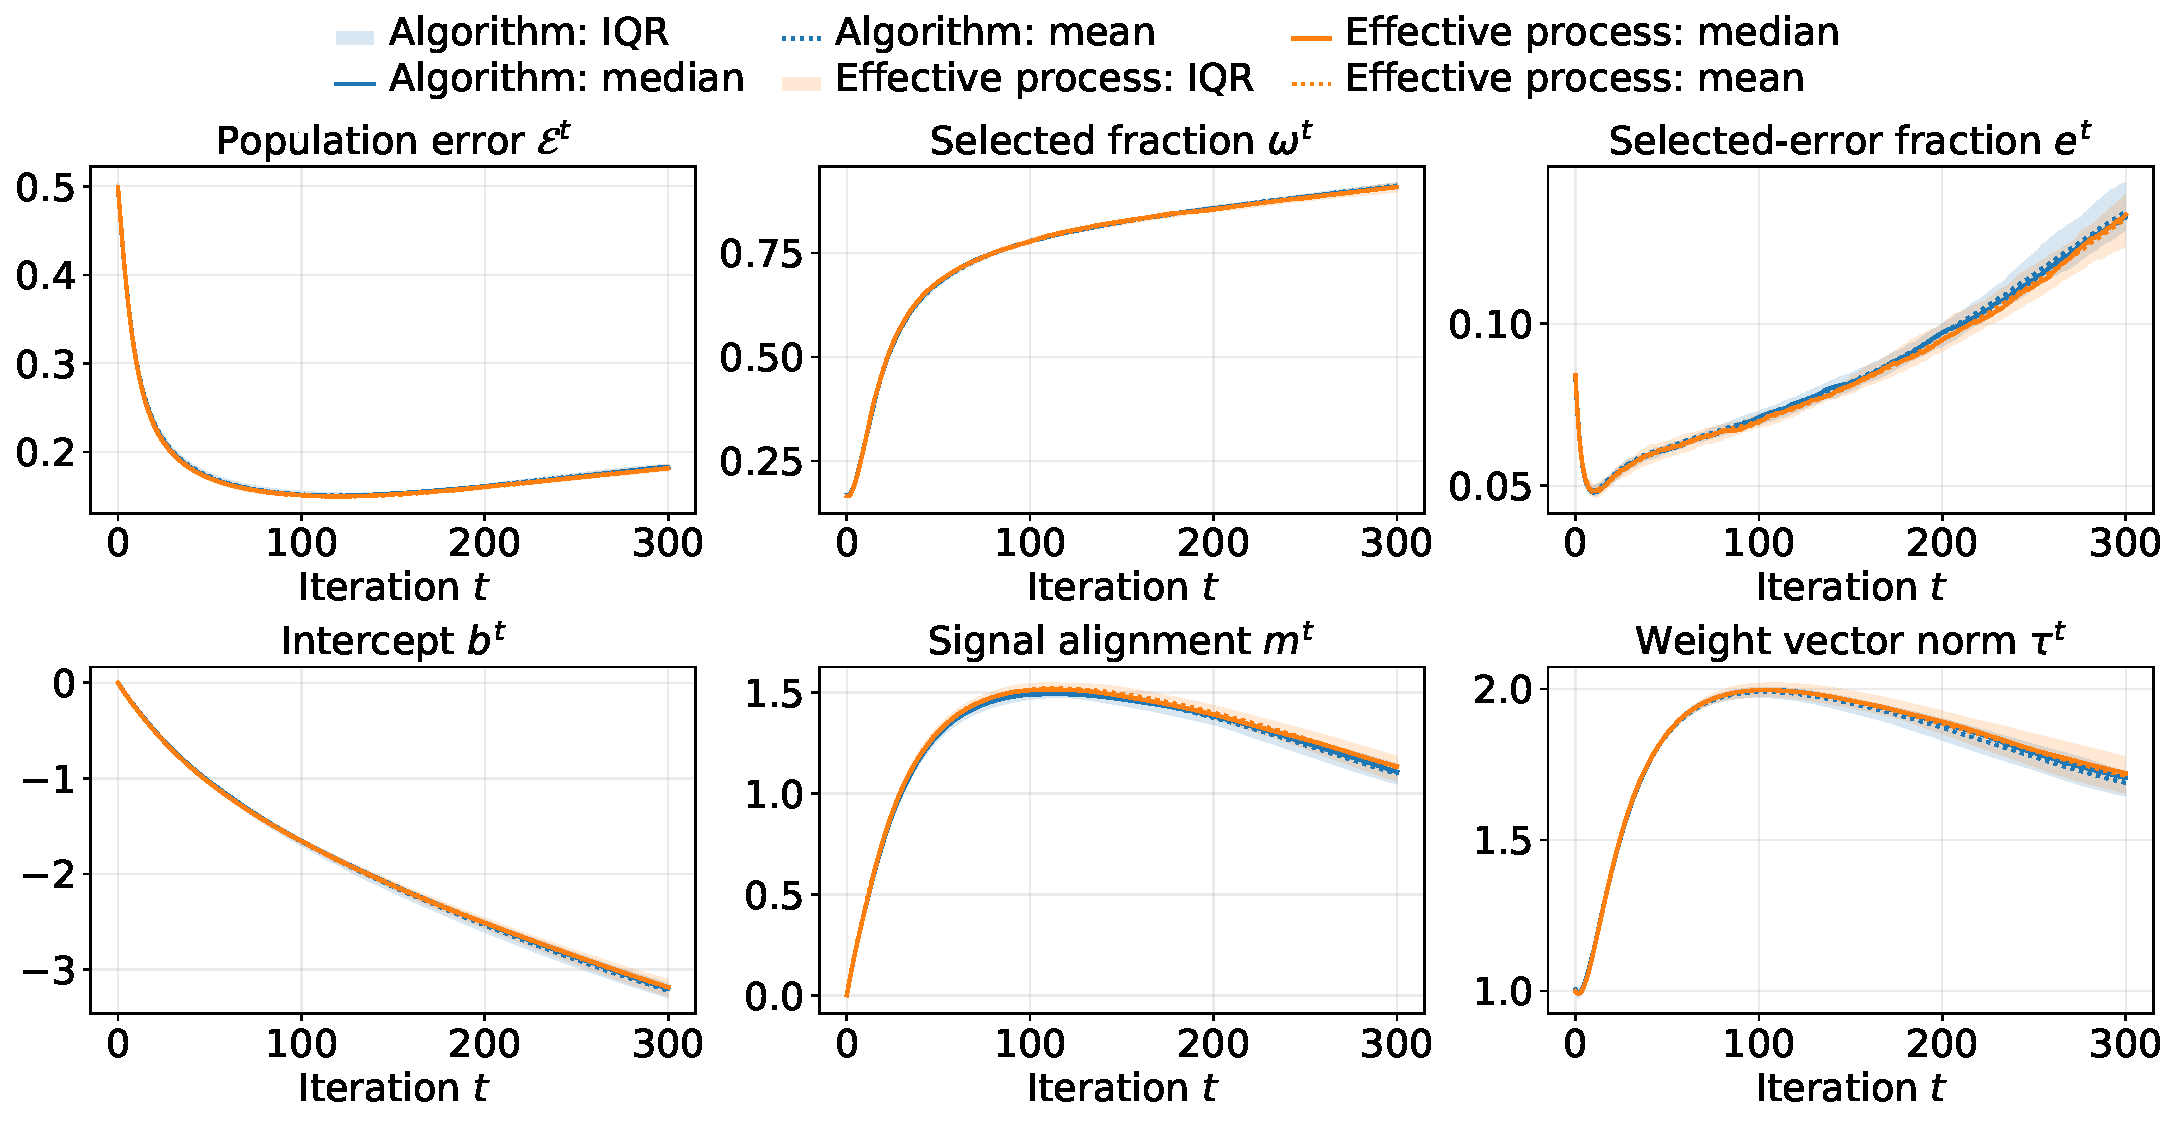
\includegraphics[width=1.0\textwidth]{approximation_accuracy.pdf} 
    
\caption{
Comparison of the self-training algorithm (blue) with the
particle approximation of the effective process (orange) over $20$ runs,
with $T=300$ iterations and seeds $42$--$61$.
Solid curves are medians, dotted curves are means, and shaded
regions are interquartile ranges.
The parameters are $d=2{,}000$, $\delta=8$, $\sigma=1$, $p=0.2$,
$\rho=0.1$, $\eta=0.1$, $\pi=5$, $\lambda=0.1$,  $\kappa_\pm=\pm\log4$, $b^{\mathrm{init}}=0$, with independent $w^{\mathrm{init}},\mu\sim\mathcal N(0_d,I_d)$.
Labels and supervision indicators are sampled independently
across observations with probabilities $p$ and $\rho$, respectively,
and held fixed throughout training.
Population errors use the configured class probability $p$.
The parameter-side and sample-side
effective processes are each simulated using $10{,}000$ particles.
}
    \label{fig:mean-field-validation} 
\end{figure}
The numerical experiments show that the effective predictions
closely track the finite-dimensional observables over the
displayed iteration horizon.
For the parameter setting and dimensions considered, this
agreement supports using the effective recursion to study
the statistical behavior of the algorithm.

\subsection{Classification error decomposition}
\label{subsec:classification-error}

By Corollary~\ref{cor:mean-field-observables}, the limiting
classification error depends on the normalized alignment
and intercept,
\[
    \bar\alpha^t
    :=
    \frac{\bar m^t}{\sigma\bar\tau^t},
    \qquad
    \bar\beta^t
    :=
    \frac{\bar b^t}{\sigma\bar\tau^t}.
\]
These are well defined at every finite time since
$\bar\tau^t>0$ by Lemma~\ref{lemma:mf-proof-nondegeneracy}.
We denote their finite-dimensional counterparts by
$\alpha^t$ and $\beta^t$, defined analogously when $\tau^t>0$.
The scalar alignment variables $\alpha^t,\bar\alpha^t$
should not be confused with the projection-coefficient
vectors $\alpha_t^{[w]},\alpha_t^{[g]}$ and their
barred counterparts.
Equation~\eqref{eq:mean-field-classification-error}
then becomes
\begin{equation}
    \bar{\mathcal E}^t
    =
    \mathcal E_{\bar p}(\bar\alpha^t,\bar\beta^t),
    \qquad
    \mathcal E_p(\alpha,\beta)
    :=
    p\,\Phi(-\alpha-\beta)
    +(1-p)\,\Phi(\beta-\alpha).
    \label{eq:normalized-classification-error}
\end{equation}
We use the Bayes classification error as a benchmark to evaluate the performance of the self-training algorithm.
Recall $\bar s_\mu=(\tilde{\mathbb E}[\tilde\mu^2])^{1/2}$
from \eqref{eq:s-mu-k-bar}, and write
$s_\mu:=\|\mu\|/\sqrt d$.

\begin{proposition}[Bayes classification error]
\label{prop:bayes-risk}
For every $\alpha>0$ and $p\in(0,1)$, the unique minimizer of
$\beta\mapsto\mathcal E_p(\alpha,\beta)$ is
\begin{equation}
    \beta_\star(\alpha;p)
    :=
    \frac{1}{2\alpha}\log\frac{p}{1-p}.
    \label{eq:classification-optimal-normalized-intercept}
\end{equation}
Suppose
Assumption~\ref{assumption:asymptotic-regime}
and Assumption~\ref{assumption:quenched-initialization} hold,
with $\bar s_\mu>0$.
For all sufficiently large $d$, the Bayes classification
error of the test mixture is
\[
    \mathcal E_{\mathrm B}
    :=
    \mathcal E_p\left(
        \frac{s_\mu}{\sigma},
        \beta_\star\left(\frac{s_\mu}{\sigma};p\right)
    \right).
\]
As $d\to\infty$, it converges to
\begin{equation}
    \bar{\mathcal E}_{\mathrm B}
    :=
    \mathcal E_{\bar p}(\alpha^\star,\beta^\star),
    \qquad
    \alpha^\star
    :=
    \frac{\bar s_\mu}{\sigma},
    \qquad
    \beta^\star
    :=
    \beta_\star(\alpha^\star;\bar p).
    \label{eq:bayes-classification-error}
\end{equation}
\end{proposition}
Next, we decompose the excess error
relative to the Bayes benchmark into alignment and intercept
regrets.
Define the smallest classification error attainable at a fixed
normalized alignment by
\[
    \mathcal E_p^{\mathrm{opt}}(\alpha)
    :=
    \inf_{\beta\in\mathbb R}
        \mathcal E_p(\alpha,\beta).
\]
For $\alpha>0$, Proposition~\ref{prop:bayes-risk} gives
\[
    \mathcal E_p^{\mathrm{opt}}(\alpha)
    =
    \mathcal E_p\bigl(\alpha,\beta_\star(\alpha;p)\bigr).
\]
For $\alpha\leq0$, the infimum equals $\min\{p,1-p\}$,
approached by predicting a single class.
Assuming $\bar s_\mu>0$, define the intercept regret and
alignment regret by
\begin{align}
    \bar{\mathcal R}_{\mathrm{int}}^t
    :=
    \mathcal E_{\bar p}(\bar\alpha^t,\bar\beta^t)
    -
    \mathcal E_{\bar p}^{\mathrm{opt}}(\bar\alpha^t),
    \qquad
    \bar{\mathcal R}_{\mathrm{align}}^t
    :=
    \mathcal E_{\bar p}^{\mathrm{opt}}(\bar\alpha^t)
    -
    \bar{\mathcal E}_{\mathrm B}.
    \label{eq:classification-regret-decomposition}
\end{align}
The intercept regret is nonnegative by definition.
Moreover, Cauchy--Schwarz gives
$|\bar\alpha^t|\leq\bar s_\mu/\sigma=\alpha^\star$.
For each fixed $\beta$,
\[
    \frac{\partial}{\partial\alpha}
        \mathcal E_p(\alpha,\beta)
    =
    -p\,\phi(\alpha+\beta)
    -(1-p)\,\phi(\beta-\alpha)
    <0,
\]
where $\phi=\Phi'$.
Thus $\mathcal E_p^{\mathrm{opt}}$ is nonincreasing, and
the alignment regret is also nonnegative.
Their sum gives the excess classification error:
\[
    \bar{\mathcal E}^t-\bar{\mathcal E}_{\mathrm B}
    =
    \bar{\mathcal R}_{\mathrm{int}}^t
    +
    \bar{\mathcal R}_{\mathrm{align}}^t.
\]
The intercept regret measures the gap between the current error
and the infimum attainable by varying the intercept while
holding the weights fixed.
The alignment regret is the remaining excess error after this
optimization.

For finite-dimensional trajectories with $\tau^t>0$,
$s_\mu>0$, and $p\in(0,1)$, the conditional test error satisfies
\[
    \mathcal E^t=\mathcal E_p(\alpha^t,\beta^t),
    \qquad
    |\alpha^t|\leq\frac{s_\mu}{\sigma}.
\]
The first identity follows from the Gaussian test-score law
used in the proof of
Corollary~\ref{cor:mean-field-observables};
the second follows from Cauchy--Schwarz.
Consequently, the same decomposition applies with
$(p,\alpha^t,\beta^t)$ and the finite-dimensional Bayes error
$\mathcal E_{\mathrm B}$ defined in
Proposition~\ref{prop:bayes-risk}, with both regret terms nonnegative.
Figure~\ref{fig:class-imbalance-regret} compares the error
trajectories and their regret decompositions in balanced and
imbalanced settings.
\begin{figure}[htbp] 
    \centering
    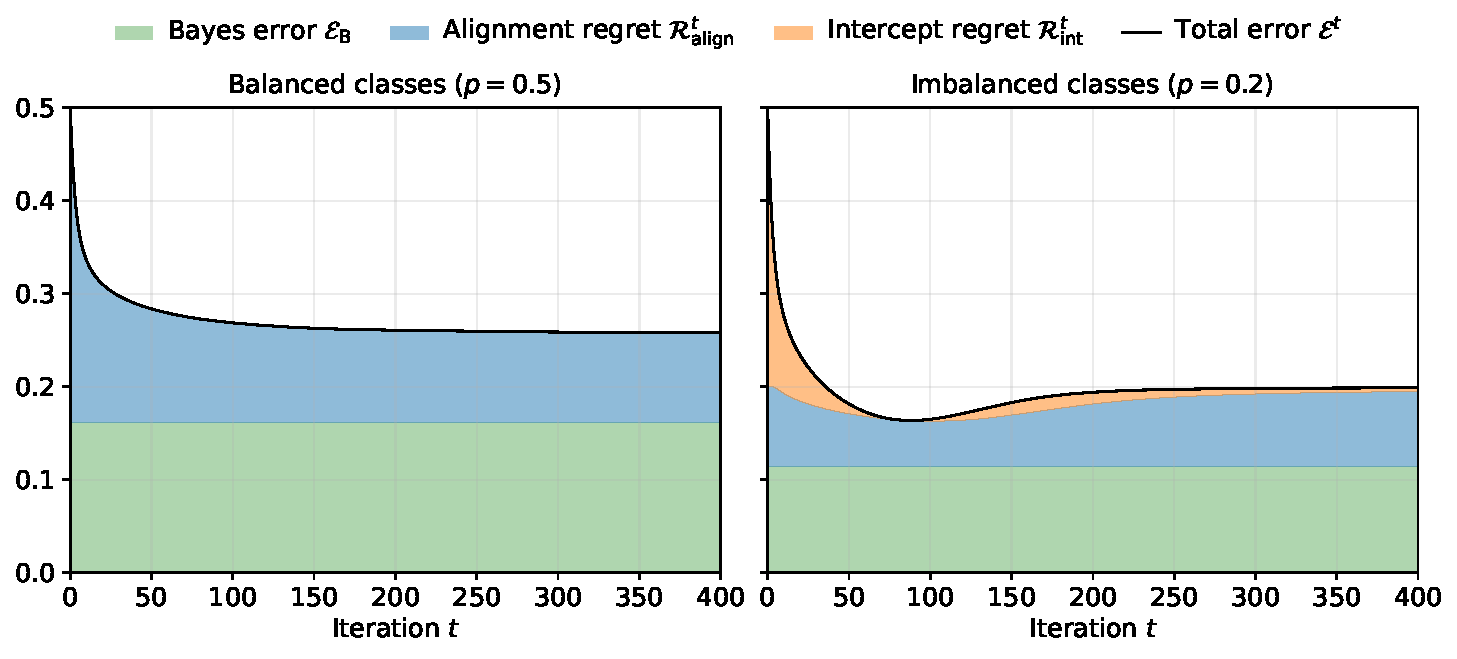
\includegraphics[width=\textwidth]{statistical_behavior_comparison.pdf} 
\caption{
Classification-error decomposition for balanced ($p=0.5$, left)
and imbalanced ($p=0.2$, right) classes, using one realization
of the self-training algorithm in each case, with $T=400$
iterations and seed $49$.
The stacked layers represent Bayes error, alignment regret,
and intercept regret; each layer's thickness gives its
contribution to the total error (black).
Both experiments use logistic loss, the quadratic penalty, $d=5{,}000$, $\delta=8$, $\sigma=1$,
$\rho=0.05$, $\eta=0.2$, $\pi=2$, $\lambda=0.1$, $\kappa_\pm=\pm\log4$, $b^{\mathrm{init}}=0$, with independent $w^{\mathrm{init}},\mu\sim\mathcal N(0_d,I_d)$.
Labels and supervision indicators are sampled independently
across observations with probabilities $p$ and $\rho$, respectively,
and held fixed throughout training.
Population errors use the configured class probability $p$.
}
\label{fig:class-imbalance-regret} 
\end{figure}

\subsection{Intercept dynamics and class imbalance}
\label{subsec:intercept-dynamics}

Our experiments show that the classification performance of
self-training depends strongly on the hyperparameters and
the data distribution, consistent with previous empirical
evaluations of self-training and semi-supervised learning
\cite{oliver2018realistic,su2021realistic}.

In balanced settings, our experiments show that classification error decreases consistently throughout training.
In imbalanced experiments, however, we repeatedly observe an
initial decrease followed by an increase, producing a U-shaped
error curve over the training iterations.
Figure~\ref{fig:class-imbalance-regret} illustrates these
contrasting trajectories.
Similar risk trajectories arise in the self-training regression
model of Wu et al.~\cite{wu2026selftraininghelpshurtsdenoising}.
In our imbalanced experiments, intercept regret begins
increasing before alignment regret.
We also observe that the normalized intercept moves beyond
its classification-optimal value as training progresses.
Figure~\ref{fig:mean-field-validation}, which uses a related
imbalanced configuration, shows the evolution of the
intercept, signal alignment, and weight norm.
Meanwhile, classification error approaches the majority-class
benchmark, equal to $0.2$ in the right panel of
Figure~\ref{fig:class-imbalance-regret}.
Together, these observations suggest an important role for
intercept feedback in the deterioration observed under
class imbalance.

The importance of intercept dynamics is also emphasized by
Takahashi~\cite{takahashi2026role}, who studies self-training
on imbalanced Gaussian mixtures using fresh unlabeled batches
and stagewise minimization, and proposes fixing the intercept
as a heuristic.
Takanami et al.~\cite{takanami2025effect} also study intercept
drift and bias fixing under imbalance in a repeated-data
self-distillation setting. 
These considerations motivate a closer examination of the
intercept and weight updates.
The following proposition distinguishes the contributions
of pseudo-label imbalance and pseudo-label correctness.

\begin{proposition}[Weighted pseudo-label contributions]
\label{prop:weighted-pseudo-label-contributions}
Suppose the hypotheses of Theorem~\ref{theorem:trajectory} hold
and, in addition,
\[
    -y\ell'(y,r)\geq0,
    \qquad
    y\in\{-1,+1\},\quad r\in\mathbb R.
\]
For every finite $t\geq0$, define
\[
    \tilde A^t
    :=
    -\tilde{\mathfrak c}^{\,t}
        \ell'(\tilde{\mathfrak c}^{\,t},\tilde r^t)
    \geq0,
\]
using the convention $\ell'(0,r)=0$.
Then the following identities hold.
Their algebra does not require the sign condition;
that condition ensures $\tilde A^t\geq0$ and supports
the subsequent interpretation.

\begin{enumerate}[label=(\roman*),wide]
    \item \emph{Weighted pseudo-label contributions.}
    The unlabeled residual satisfies
    \begin{align}
        \tilde{\mathbb E}[\tilde g_{\mathcal U}^t]
        &=
        \tilde{\mathbb E}\left[
            \tilde A^t
            \left(
                \mathbf1_{\{\tilde{\mathfrak c}^{\,t}=-1\}}
                -
                \mathbf1_{\{\tilde{\mathfrak c}^{\,t}=+1\}}
            \right)
            \,\middle|\,\tilde\Delta=0
        \right],
        \label{eq:weighted-pseudo-label-imbalance}
        \\
        \tilde{\mathbb E}
            [\tilde Y\tilde g_{\mathcal U}^t]
        &=
        \tilde{\mathbb E}\left[
            \tilde A^t
            \left(
                \mathbf1_{\{\tilde{\mathfrak c}^{\,t}=-\tilde Y\}}
                -
                \mathbf1_{\{\tilde{\mathfrak c}^{\,t}=\tilde Y\}}
            \right)
            \,\middle|\,\tilde\Delta=0
        \right].
        \label{eq:weighted-pseudo-label-correctness}
    \end{align}
    For logistic loss,
    \[
        \tilde A^t
        =
        \frac{|\tilde{\mathfrak c}^{\,t}|}
             {1+e^{|\tilde r^t|}}.
    \]

    \item \emph{Intercept and overlap updates.}
    Writing
    \[
        \bar\zeta^t
        =
        \tilde{\mathbb E}[\tilde g_{\mathcal L}^t]
        +
        \pi\tilde{\mathbb E}[\tilde g_{\mathcal U}^t],
        \qquad
        \bar\chi^t
        =
        \tilde{\mathbb E}[\tilde Y\tilde g_{\mathcal L}^t]
        +
        \pi\tilde{\mathbb E}[\tilde Y\tilde g_{\mathcal U}^t],
    \]
    Definition~\ref{def:mean-field-recursion} gives
    \begin{equation}
        \bar b^{t+1}-\bar b^t
        =
        -\eta\bar\zeta^t
        \label{eq:statistical-intercept-drift}
    \end{equation}
    and
    \begin{equation}
        \bar m^{t+1}-\bar m^t
        =
        -\eta\left[
            \bar\chi^t\bar s_\mu^2
            +
            \lambda
            \tilde{\mathbb E}
                [\tilde\mu\,j'(\tilde w^t)]
            +
            \sigma
            \sum_{s=0}^{t}
                \bar\gamma^{[g]}(t,s)\bar m^s
        \right].
        \label{eq:statistical-overlap-update}
    \end{equation}
\end{enumerate}
\end{proposition}

Equation~\eqref{eq:weighted-pseudo-label-imbalance}
measures the derivative-weighted imbalance between negative
and positive selected pseudo-labels.
Its contribution to the intercept increment is
$-\eta\pi\tilde{\mathbb E}[\tilde g_{\mathcal U}^t]$.
Thus, when $\pi>0$, a larger weighted mass of negative
pseudo-labels pushes the intercept downward, whereas a larger
weighted mass of positive pseudo-labels pushes it upward.
Equation~\eqref{eq:weighted-pseudo-label-correctness}
instead compares incorrect and correct selected pseudo-labels.
Through the explicit signal term
$-\eta\pi\tilde{\mathbb E}
[\tilde Y\tilde g_{\mathcal U}^t]\tilde\mu$,
correct pseudo-labels contribute toward the signal and
incorrect pseudo-labels contribute in the opposite direction.
The complete overlap update
\eqref{eq:statistical-overlap-update} also contains the labeled
contribution, regularization, and memory.
For a quadratic penalty, $j(u)=u^2/2$, its regularization
expectation reduces to $\bar m^t$.
These identities distinguish the quantities driving the updates,
but explaining intercept overshoot requires understanding
how the weighted pseudo-label imbalance evolves jointly
with the weights.
This raises the question:

\medskip
\emph{Under what conditions does self-training drive the
normalized intercept beyond its classification-optimal value,
and how does this interact with signal alignment and
classification error?}
\medskip

The effective recursion characterizes the transient dynamics,
but extracting an analytical explanation of intercept
amplification remains challenging.
Its coefficients depend self-consistently on the trajectory
laws, while nonlinear feedback and memory prevent a closed
description in terms of the intercept and alignment alone.
Long-time convergence and equilibrium behavior of effective
processes have been studied in
\cite{celentano2026highdimensionalasymptoticsordermethods,
fan2025dynamicalmeanfieldanalysisadaptivereplica,
chen2025learningsingleindexmodel};
Theorem~\ref{thm:effective-process-convergence} also establishes
convergence for the present recursion.
These convergence results do not by themselves provide
quantitative conditions for intercept amplification.
We leave such a characterization under class imbalance
as an open problem.

Nevertheless, an exact reference case arises when the classes
are balanced within both supervision populations, the thresholds
are symmetric, and the initial effective intercept is zero.
Under a corresponding symmetry of the loss, the labeled and
unlabeled contributions to the intercept update each vanish
at every iteration.

\begin{proposition}[Preservation of a zero intercept under symmetry]
\label{prop:zero-intercept-symmetry}
Suppose the hypotheses of Theorem~\ref{theorem:trajectory}
hold. Assume that the loss satisfies
\begin{equation}
    \ell'(-y,-r)=-\ell'(y,r),
    \quad y\in\{-1,+1\},\quad r\in\mathbb R,
    \label{eq:loss-label-score-symmetry}
\end{equation}
and that the classes are balanced within each supervision
population:
\begin{equation}
    \tilde{\mathbb P}(\tilde Y=+1\mid\tilde\Delta=a)
    =\frac12,
    \qquad a\in\{0,1\}.
    \label{eq:balance-within-supervision}
\end{equation}
If $\kappa_-=-\kappa_+$ and $\bar b^0=0$,
then, for every $t\geq0$,
\begin{equation}
    \bar b^t=0,
    \qquad
    \tilde{\mathbb E}[\tilde g_{\mathcal L}^t]
    =
    \tilde{\mathbb E}[\tilde g_{\mathcal U}^t]
    =0.
    \label{eq:zero-intercept-all-times}
\end{equation}
Moreover, for every finite horizon $T$,
\begin{equation}
    (\tilde Y,\tilde\Delta,\tilde r^0,\ldots,\tilde r^T)
    \overset{\mathrm d}{=}
    (-\tilde Y,\tilde\Delta,-\tilde r^0,\ldots,-\tilde r^T).
    \label{eq:joint-score-reflection}
\end{equation}
\end{proposition}

Every differentiable margin loss
$\ell(y,r)=\varphi(yr)$ satisfies
\eqref{eq:loss-label-score-symmetry}, since
$\ell'(y,r)=y\varphi'(yr)$; this includes logistic loss.
Under the hypotheses of
Proposition~\ref{prop:zero-intercept-symmetry},
$\bar p=1/2$ and $\bar\beta^t=0$, so
\begin{equation}
    \bar{\mathcal E}^t=\Phi(-\bar\alpha^t).
    \label{eq:symmetric-classification-error}
\end{equation}
Classification performance is therefore determined entirely
by normalized alignment. At times when $\bar\alpha^t\geq0$,
the intercept regret vanishes. Any deterioration in the
effective classification error must be accompanied by a
decrease in $\bar\alpha^t$.
For the finite-dimensional iterates,
Theorem~\ref{theorem:trajectory} also gives
\[
    \max_{0\leq t\leq T}|b^t|
    \xrightarrow{\mathbb P}0
\]
for every fixed finite horizon $T$.
Thus exact preservation of the effective intercept corresponds
to an asymptotically vanishing finite-dimensional intercept
on fixed horizons.


\bibliographystyle{plain}
\bibliography{references}

\appendix

\section{Proofs from Section \ref{subsec:finite-dim}}
\label{sec:proof-finite-dim}

Throughout this section,
Assumption~\ref{assumption:finite-dim-loss-penalty} holds.
We first prove the intermediate propositions in
Section~\ref{subsec:proof-intermediate-res-finite-dim},
then establish global descent in
Section~\ref{subsec:global-descent}, finite branch identification
in Section~\ref{subsec:branch-identification}, and convergence
in Section~\ref{subsec:convergence-within-branch}.

\subsection{Proof of intermediate results}
\label{subsec:proof-intermediate-res-finite-dim}

\begin{proof}[Proof of Proposition~\ref{prop:ST-potential}]
Direct integration gives
\begin{equation}
    \Psi_\kappa(r)
    =
    \begin{cases}
        \ell(-1,r)-\ell(-1,\kappa_-),
            & r\leq\kappa_-,\\
        0,
            & \kappa_-<r<\kappa_+,\\
        \ell(+1,r)-\ell(+1,\kappa_+),
            & r\geq\kappa_+.
    \end{cases}
    \label{eq:psi-kappa-formula}
\end{equation}
Nonnegativity and monotonicity of the loss give
\begin{align}
    -C_\kappa\leq\Psi_\kappa\leq0,
    \qquad
    C_\kappa:=
    \max\{\ell(-1,\kappa_-),\ell(+1,\kappa_+)\}. \label{eq:c-kappa}
\end{align}
Thus $\Psi_\kappa$ is bounded and continuous, and is twice
continuously differentiable away from the thresholds.
Convexity and the derivative signs give
\[
    |\psi_\kappa(r)|
    \leq
    \max\{\ell'(-1,\kappa_-),-\ell'(+1,\kappa_+)\}
    <\infty,
\]
so its integral $\Psi_\kappa$ is globally Lipschitz.

Since the supervised loss and penalty are $C^2$, it follows that
$V$ is continuous and $C^2$ outside $\mathcal S_\kappa$.
There, the chain rule gives
\[
    \nabla V(\theta)
    =
    \nabla L_{\mathcal L}(\theta)
    +
    \frac{\pi}{M}\sum_{j\in I_{\mathcal U}}
        \psi_\kappa(r_j(\theta))\breve X_j
    +
    \frac{\lambda}{d}
        \begin{bmatrix}0\\\nabla J(w)\end{bmatrix}
    =
    G(\theta).
\]
Each threshold equation defines a proper affine hyperplane,
since the coefficient of $b$ in $r_j(\theta)$ is one, and
their finite union has Lebesgue measure zero.
\end{proof}

\begin{proof}[Proof of Proposition~\ref{prop:configuration-branch-formulation}]
By the selection convention, $\theta\in\Theta_{\mathfrak c}$
if and only if, for every $j\in I_{\mathcal U}$,
\[
    \begin{cases}
        r_j(\theta)\leq\kappa_-,
            & \mathfrak c_j=-1,\\
        \kappa_-<r_j(\theta)<\kappa_+,
            & \mathfrak c_j=0,\\
        r_j(\theta)\geq\kappa_+,
            & \mathfrak c_j=+1.
    \end{cases}
\]
Hence each branch is convex.
For a nonempty branch, its closure is obtained by replacing
the strict inequalities by non-strict ones.
Indeed, fix a point in the branch and interpolate it with
any point satisfying these weak inequalities.
Every interpolant with positive weight on the branch point
satisfies the strict inequalities and remains in the branch.
The weak-inequality set is closed, proving the claimed
closure characterization. It is therefore polyhedral.
The partition property follows from the definition of
$\mathfrak C$, whose range contains at most $3^M$ configurations.

The explicit formula \eqref{eq:psi-kappa-formula} gives
$V=L_{\mathfrak c}+K_{\mathfrak c}$ on $\Theta_{\mathfrak c}$,
where
\[
    K_{\mathfrak c}
    :=
    -\frac{\pi}{M}
    \left[
        \#\{j\in I_{\mathcal U}:\mathfrak c_j=-1\}
            \ell(-1,\kappa_-)
        +
        \#\{j\in I_{\mathcal U}:\mathfrak c_j=+1\}
            \ell(+1,\kappa_+)
    \right].
\]
Continuity extends the identity to
$\overline{\Theta_{\mathfrak c}}$.
Finally, for every $\vartheta\in\Theta_{\mathfrak c}$,
\[
    L_{\mathrm{ST}}(\theta;\vartheta)
    =
    L_{\mathfrak c}(\theta)
    \qquad\text{for every }\theta.
\]
Differentiating with respect to $\theta$ and then setting
$\vartheta=\theta\in\Theta_{\mathfrak c}$ gives
$G(\theta)=\nabla L_{\mathfrak c}(\theta)$, including at thresholds
assigned to that branch.
\end{proof}

\begin{proof}[Proof of Proposition~\ref{prop:branch-convexity-coercivity}]
By Assumption~\ref{assumption:finite-dim-loss-penalty},
$\ell''(y,r)>0$ and $j''(u)>0$.
Since $\pi\geq0$, for every nonzero direction
$(a,u)\in\mathbb R\times\mathbb R^d$,
\[
    \begin{bmatrix}a\\u\end{bmatrix}^{\!\top}
    \nabla^2L_{\mathfrak c}(\theta)
    \begin{bmatrix}a\\u\end{bmatrix}
    \geq
    \frac1N\sum_{i\in I_{\mathcal L}}
        \ell''(Y_i,r_i(\theta))
        \left(a+\frac{X_i^\top u}{\sqrt d}\right)^2
    +
    \frac{\lambda}{d}\sum_{k=1}^d j''(w_k)u_k^2
    >0.
\]
Indeed, the penalty term is positive when $u\neq0$, while the
labeled term is positive when $u=0$ and $a\neq0$.
Thus every branch Hessian is positive definite, and every
$L_{\mathfrak c}$ is strictly convex.
Moreover, $\ell''\leq L_\ell$, $j''\leq L_j$, and $\pi\geq0$
imply
\[
    \nabla^2L_{\mathfrak c}(\theta)\preceq H_d.
\]
Indeed, the unlabeled Hessian contribution is bounded by
enlarging its sum to all unlabeled observations.

The sublevel sets of the supervised objective
$L_{\mathcal L}(\theta)+(\lambda/d)J(w)$ bound $w$
through the nonnegative, coercive penalty.
Convexity and the strict derivative signs imply
\[
    \ell(-1,r)\longrightarrow+\infty
        \quad\text{as }r\longrightarrow+\infty,
    \qquad
    \ell(+1,r)\longrightarrow+\infty
        \quad\text{as }r\longrightarrow-\infty.
\]
With $w$ bounded, a negative labeled observation therefore prevents
$b\to+\infty$, and a positive labeled observation prevents
$b\to-\infty$.
The supervised objective is consequently coercive.
Every $L_{\mathfrak c}$ is bounded below by this objective,
while $V$ differs from it by a bounded term.
Consequently, both are coercive.
Continuity gives existence of each branch minimizer, and
strict convexity gives uniqueness.
\end{proof}

\subsection{Proof of Theorem~\ref{thm:st-convergence}}

\subsubsection{Global descent}
\label{subsec:global-descent}

\begin{lemma}[Global descent and boundedness]
\label{lem:st-global-descent-boundedness}
For $\pi,\lambda\geq0$, the potential satisfies
\begin{equation}
    V(\theta+h)-V(\theta)
    \leq
    G(\theta)^\top h+\frac12h^\top H_dh,
    \qquad \theta,h\in\mathbb R^{d+1}.
    \label{eq:st-global-quadratic-upper-bound}
\end{equation}
Under \eqref{eq:st-descent-step-size}, set
$c_d:=\eta(1-\eta\Lambda_d/2)>0$.
Then the iterates satisfy
\begin{equation}
    V(\theta^{t+1})-V(\theta^t)
    \leq
    -c_d\|P_d^{1/2}G(\theta^t)\|^2,
    \qquad t\geq1,
    \label{eq:st-global-descent}
\end{equation}
and $G(\theta^t)\to0$.
If, in addition, $\lambda>0$ and both classes occur in the
labeled sample, then the trajectory is bounded.
\end{lemma}
\begin{proof}
Since $\ell''(y,r)\leq L_\ell$, for every $r,\delta\in\mathbb R$,
\[
    \ell(y,r+\delta)
    \leq
    \ell(y,r)+\ell'(y,r)\delta+\frac{L_\ell}{2}\delta^2.
\]
On each smooth interval,
$0\leq\psi_\kappa'(u)\leq L_\ell$.
The signs
$\ell'(-1,\kappa_-)>0$ and $\ell'(+1,\kappa_+)<0$
give a downward jump at each threshold.
With the prescribed values at the thresholds,
$u\mapsto\psi_\kappa(u)-L_\ell u$ is nonincreasing.
Therefore
\[
    (\psi_\kappa(v)-\psi_\kappa(u))(v-u)
    \leq L_\ell(v-u)^2,
    \qquad u,v\in\mathbb R.
\]
The definition of $\Psi_\kappa$ gives
\begin{align*}
    \Psi_\kappa(r+\delta)-\Psi_\kappa(r)
        -\psi_\kappa(r)\delta
    =
    \int_0^1[\psi_\kappa(r+s\delta)-\psi_\kappa(r)]
        \delta\,ds
    \leq
    \int_0^1L_\ell s\delta^2\,ds
    =
    \frac{L_\ell}{2}\delta^2.
\end{align*}
For $s>0$, the integrand bound follows by applying the preceding
inequality with $u=r$ and $v=r+s\delta$, then dividing by $s$.
The argument holds for either sign of $\delta$ and across thresholds.

Apply these scalar bounds with $\delta=\breve X_i^\top h$.
Writing $h=(h_b,h_w)\in\mathbb R\times\mathbb R^d$, also use
\[
    J(w+h_w)-J(w)
    \leq
    \nabla J(w)^\top h_w+\frac{L_j}{2}\|h_w\|^2.
\]
Summing, with $\pi,\lambda\geq0$, proves
\eqref{eq:st-global-quadratic-upper-bound}.
Substituting $h=-\eta P_dG(\theta^t)$ and using the definition of
$\Lambda_d$ yields \eqref{eq:st-global-descent}.
In particular, the potential decreases strictly at every
nonstationary iteration, including iterations that cross
branch boundaries.

The potential is bounded below because $\Psi_\kappa$ is bounded
and the loss and penalty are nonnegative.
Summing the descent inequality therefore gives
\[
    c_d\sum_{t=1}^T\|P_d^{1/2}G(\theta^t)\|^2
    \leq V(\theta^1)-V(\theta^{T+1})
    \leq V(\theta^1)-\inf_\theta V(\theta)<\infty.
\]
Consequently, writing
$\Delta\theta^t:=\theta^{t+1}-\theta^t$,
\begin{equation}
    \sum_{t=1}^\infty\|P_d^{1/2}G(\theta^t)\|^2<\infty,
    \qquad
    \sum_{t=1}^\infty\|\Delta\theta^t\|_{P_d^{-1}}^2<\infty,
    \label{eq:st-square-summable-updates}
\end{equation}
where the second sum is $\eta^2$ times the first.
For fixed $d$, invertibility of $P_d$ and the update identity imply
\begin{equation}
    G(\theta^t)\xrightarrow[t\to\infty]{}0,
    \qquad
    \Delta\theta^t=-\eta P_dG(\theta^t)
        \xrightarrow[t\to\infty]{}0.
    \label{eq:parameter-difference-converges-to-zero}
\end{equation}
If $\lambda>0$ and both classes occur in the labeled sample,
Proposition~\ref{prop:branch-convexity-coercivity} gives coercivity
of $V$. By descent, the iterates from $t=1$ onward remain in
the compact sublevel set
\[
    \{\theta\in\mathbb R^{d+1}:V(\theta)\leq V(\theta^1)\}.
\]
Thus the trajectory is bounded.
\end{proof}

\subsubsection{Branch identification}
\label{subsec:branch-identification}

\begin{lemma}[Finite branch identification]
\label{lem:st-finite-identification}
Suppose $\pi>0$.
If a trajectory of \eqref{eq:ST-recursion-G} is bounded and satisfies
$G(\theta^t)\to0$, then there are a finite time
$T_{\mathrm{id}}\geq1$ and a nonempty branch
$\Theta_{\mathfrak c}$ such that
\begin{equation}
    \mathfrak C(\theta^t)=\mathfrak c,
    \qquad t\geq T_{\mathrm{id}}.
    \label{eq:st-finite-branch-identification}
\end{equation}
\end{lemma}

\begin{proof}
We first show that gradients of distinct branches cannot coincide
at a point belonging to both branch closures.
Let $\Theta_{\mathfrak c}$ and $\Theta_{\mathfrak d}$ be nonempty,
distinct branches, and let
\[
    \theta^\star\in
        \overline{\Theta_{\mathfrak c}}
        \cap\overline{\Theta_{\mathfrak d}},
    \qquad
    D_{\mathfrak c,\mathfrak d}
    :=
    \{j\in I_{\mathcal U}:\mathfrak c_j\neq\mathfrak d_j\}.
\]
Since $\kappa_-<\kappa_+$, the closures of the negative and positive
selection regions are disjoint.
Thus, for each $j\in D_{\mathfrak c,\mathfrak d}$, exactly one of
$\mathfrak c_j,\mathfrak d_j$ is zero, and $r_j(\theta^\star)$
equals the threshold corresponding to the nonzero state.

Set
\[
    \alpha_j
    :=
    \left|
        \ell'\bigl(
            \operatorname{sign}(r_j(\theta^\star)),
            r_j(\theta^\star)
        \bigr)
    \right|
    >0,
    \qquad j\in D_{\mathfrak c,\mathfrak d}.
\]
The supervised and penalty gradients, and the unlabeled terms
with equal states, cancel. Since the nonzero state has the same
sign as $r_j(\theta^\star)$, the derivative signs give
\[
    \nabla L_{\mathfrak c}(\theta^\star)
    -
    \nabla L_{\mathfrak d}(\theta^\star)
    =
    -\frac{\pi}{M}
    \sum_{j\in D_{\mathfrak c,\mathfrak d}}
        (\mathfrak c_j-\mathfrak d_j)\alpha_j\breve X_j.
\]
Choose $\theta_{\mathfrak c}\in\Theta_{\mathfrak c}$ and
$\theta_{\mathfrak d}\in\Theta_{\mathfrak d}$.
The branch inequalities imply
\[
    (\mathfrak c_j-\mathfrak d_j)
    \bigl(
        r_j(\theta_{\mathfrak c})
        -
        r_j(\theta_{\mathfrak d})
    \bigr)
    =
    |r_j(\theta_{\mathfrak c})-r_j(\theta_{\mathfrak d})|
    >0,
    \qquad j\in D_{\mathfrak c,\mathfrak d},
\]
because the selected score lies at or beyond its threshold,
whereas the unselected score lies strictly inside the threshold
interval.
Taking the inner product with
$\theta_{\mathfrak c}-\theta_{\mathfrak d}$ therefore gives
\begin{equation}
\begin{aligned}
    \bigl(
        \nabla L_{\mathfrak c}(\theta^\star)
        -
        \nabla L_{\mathfrak d}(\theta^\star)
    \bigr)^\top
    (\theta_{\mathfrak c}-\theta_{\mathfrak d})
    =
    -\frac{\pi}{M}
    \sum_{j\in D_{\mathfrak c,\mathfrak d}}
        \alpha_j
        |r_j(\theta_{\mathfrak c})-r_j(\theta_{\mathfrak d})|
    <0.
\end{aligned}
    \label{eq:st-branch-gradient-separation}
\end{equation}
Strictness follows from $\pi>0$,
$D_{\mathfrak c,\mathfrak d}\neq\varnothing$, and $\alpha_j>0$.

If configurations changed infinitely often, finiteness of the
configuration set would give distinct configurations
$\mathfrak c,\mathfrak d$ and times $t_k\to\infty$ such that
\[
    \theta^{t_k}\in\Theta_{\mathfrak c},
    \qquad
    \theta^{t_k+1}\in\Theta_{\mathfrak d}.
\]
By boundedness, after passing to a subsequence,
$\theta^{t_k}\to\theta^\star$.
The update identity and $G(\theta^t)\to0$ imply
$\theta^{t+1}-\theta^t\to0$, so
$\theta^{t_k+1}\to\theta^\star$ as well.
Hence $\theta^\star$ belongs to both branch closures.
By Proposition~\ref{prop:configuration-branch-formulation}
and continuity of the branch gradients,
\[
    \nabla L_{\mathfrak c}(\theta^\star)
    =
    \lim_{k\to\infty}G(\theta^{t_k})=0,
    \qquad
    \nabla L_{\mathfrak d}(\theta^\star)
    =
    \lim_{k\to\infty}G(\theta^{t_k+1})=0.
\]
This contradicts \eqref{eq:st-branch-gradient-separation}.
There are therefore only finitely many configuration changes,
proving \eqref{eq:st-finite-branch-identification}.
\end{proof}

\subsubsection{Convergence within the identified branch}
\label{subsec:convergence-within-branch}

\begin{proof}[Proof of Theorem~\ref{thm:st-convergence}]
Lemma~\ref{lem:st-global-descent-boundedness} gives boundedness and
$G(\theta^t)\to0$.
Lemma~\ref{lem:st-finite-identification} then gives
$T_{\mathrm{id}}<\infty$.
For the identified branch $\Theta_{\mathfrak c}$,
Proposition~\ref{prop:configuration-branch-formulation} yields
\[
    \theta^{t+1}
    =
    \theta^t-\eta P_d\nabla L_{\mathfrak c}(\theta^t),
    \qquad t\geq T_{\mathrm{id}}.
\]
Boundedness guarantees at least one accumulation point.
Every such point belongs to $\overline{\Theta_{\mathfrak c}}$
and is a zero of $\nabla L_{\mathfrak c}$, by continuity of the
branch gradient and $G(\theta^t)\to0$.
By Proposition~\ref{prop:branch-convexity-coercivity},
every accumulation point therefore equals the unique global
minimizer $\theta_{\mathfrak c}^\star$.
Consequently,
\begin{equation}
    \theta^t\longrightarrow\theta_{\mathfrak c}^\star,
    \qquad
    \nabla L_{\mathfrak c}(\theta_{\mathfrak c}^\star)=0,
    \qquad
    \theta_{\mathfrak c}^\star
        \in\overline{\Theta_{\mathfrak c}}.
    \label{eq:st-branch-limit}
\end{equation}
For the geometric rate, work in the coordinates
$x^t=P_d^{-1/2}\theta^t$ and define
\[
    T_{\mathfrak c}(x)
    :=
    x-\eta P_d^{1/2}
        \nabla L_{\mathfrak c}(P_d^{1/2}x),
    \qquad
    x_{\mathfrak c}^\star
    :=
    P_d^{-1/2}\theta_{\mathfrak c}^\star.
\]
Then $x^{t+1}=T_{\mathfrak c}(x^t)$ for
$t\geq T_{\mathrm{id}}$, and
$T_{\mathfrak c}(x_{\mathfrak c}^\star)
=x_{\mathfrak c}^\star$.
Let
\[
    K
    :=
    \overline{\operatorname{conv}}
    \left(
        \{x^t:t\geq T_{\mathrm{id}}\}
        \cup\{x_{\mathfrak c}^\star\}
    \right).
\]
Boundedness of the trajectory implies that $K$ is compact.
For $x\in K$, write
\[
    A(x)
    :=
    P_d^{1/2}
        \nabla^2L_{\mathfrak c}(P_d^{1/2}x)
    P_d^{1/2}.
\]
The branch Hessian is continuous and positive definite
everywhere. Compactness therefore gives
\[
    m_K
    :=
    \min_{x\in K}\lambda_{\min}(A(x))
    >0.
\]
Moreover, the upper Hessian bound and the definition of
$\Lambda_d$ give
\[
    m_K I_{d+1}
    \preceq A(x)
    \preceq \Lambda_d I_{d+1},
    \qquad x\in K.
\]
Since
\(
    DT_{\mathfrak c}(x)
    =
    I_{d+1}-\eta A(x)
\),
the step-size condition \eqref{eq:st-descent-step-size}
implies
\[
    \sup_{x\in K}
        \|DT_{\mathfrak c}(x)\|_{\mathrm{op}}
    \leq
    \max\{|1-\eta m_K|,\ |1-\eta\Lambda_d|\}
    <1.
\]
Choose $q\in(0,1)$ bounding the left-hand side.
Convexity of $K$ and the integral form of the mean-value
formula yield
\[
    T_{\mathfrak c}(x)-T_{\mathfrak c}(y)
    =
    \int_0^1
        DT_{\mathfrak c}(y+s(x-y))(x-y)\,ds,
    \qquad x,y\in K,
\]
and hence
\begin{equation}
    \|T_{\mathfrak c}(x)-T_{\mathfrak c}(y)\|
    \leq q\|x-y\|,
    \qquad x,y\in K.
    \label{eq:st-branch-contraction}
\end{equation}
The set $K$ need not lie inside the identified branch:
the smooth map $T_{\mathfrak c}$ is defined everywhere,
and the actual iterates already remain in that branch.
Applying \eqref{eq:st-branch-contraction} with
$x=x^t$ and $y=x_{\mathfrak c}^\star$ gives
\[
    \|x^{t+1}-x_{\mathfrak c}^\star\|
    \leq q\|x^t-x_{\mathfrak c}^\star\|,
    \qquad t\geq T_{\mathrm{id}}.
\]
Iteration and the identity
$\|P_d^{-1/2}v\|=\|v\|_{P_d^{-1}}$ now give
\[
    \|\theta^t-\theta_{\mathfrak c}^\star\|_{P_d^{-1}}
    \leq
    q^{\,t-T_{\mathrm{id}}}
    \|\theta^{T_{\mathrm{id}}}
        -\theta_{\mathfrak c}^\star\|_{P_d^{-1}},
    \qquad t\geq T_{\mathrm{id}}.
\]
Finally,
\[
    \|\theta^{t+1}-\theta^t\|_{P_d^{-1}}
    \leq
    (1+q)q^{\,t-T_{\mathrm{id}}}
    \|\theta^{T_{\mathrm{id}}}
        -\theta_{\mathfrak c}^\star\|_{P_d^{-1}}.
\]
The geometric series and the finite initial segment show
that the trajectory has finite length.
\end{proof}

\section{Proofs from Section~\ref{subsec:mean-field}}
\label{sec:proof-mean-field}

Throughout this section, the hypotheses of
Theorem~\ref{theorem:trajectory} hold.
We first establish well-definedness of the recursion in
Definition~\ref{def:mean-field-recursion}
in Section~\ref{subsec:well-definedness-effective}.
We introduce notation and state the master recursion in
Section~\ref{subsec:notation-master-rec}.
After proving the supporting lemmas in
Section~\ref{subsec:supporting-lem}, we establish the master
recursion in Section~\ref{subsec:proof-master-rec}
and deduce the trajectory theorem and its corollary in
Section~\ref{subsec:proof-trajectory}.
Fix $T\in\mathbb N$.

\subsection{Well-definedness of the effective process}
\label{subsec:well-definedness-effective}

For $a\in\{w,g\}$, write
\[
    \bar C_t^{[a]}
    :=
    \bigl(\bar C^{[a]}(s,u)\bigr)_{0\leq s,u\leq t},
    \qquad
    \bar\alpha_t^{[a]}
    :=
    \bigl(\bar\alpha^{[a]}(t,s)\bigr)_{0\leq s<t}.
\]
We also write
\[
    \bar\phi_t^{[w]}
    :=
    \bigl(\bar\phi^{[w]}(t,s)\bigr)_{0\leq s<t},
    \qquad
    \bar\phi_t^{[g]}
    :=
    \bigl(\bar\phi^{[g]}(t,s)\bigr)_{0\leq s\leq t}.
\]
Coefficient vectors are column vectors, and matrices and
vectors with empty index sets are understood to be empty.

\begin{lemma}[Well-definedness and positive innovations]
        \label{lemma:mf-proof-nondegeneracy}
        Under the hypotheses of Theorem~\ref{theorem:trajectory},
        the effective recursion in
        Definition~\ref{def:mean-field-recursion}
        uniquely determines the sample-side
        and parameter-side joint trajectory laws at every finite
        horizon, and all its coordinates have finite second moments. For every $t\geq0$,
        \[
            \bar C_t^{[w]}\succ0,
            \qquad
            \bar C_t^{[g]}\succ0,
            \qquad
            \bar v_t^{[w]}>0,
            \qquad
            \bar v_t^{[g]}>0.
        \]
        Moreover, $\tilde r^t$ has an absolutely continuous distribution and
        \[
            \tilde{\mathbb P}
            (\tilde r^t\in\{0,\kappa_-,\kappa_+\})=0.
        \]
        \end{lemma}

        \begin{proof}
        Fix the base variables and independent Gaussian innovation
        sequences specified in
        Definition~\ref{def:mean-field-recursion}.
        We construct the processes in the order
        \[
            \tilde w^t
            \ \longrightarrow\
            (\tilde q^t,\tilde r^t,\tilde g^t)
            \ \longrightarrow\
            (\tilde p^t,\tilde w^{t+1}).
        \]
        We use the following one-step forms of the effective fluctuations:
        \begin{align}
            \tilde q^t
            &=
            \sum_{s=0}^{t-1}
                \bar\alpha^{[w]}(t,s)\tilde q^s
            +
            \frac1{\sqrt{\bar\delta}}
            \sum_{s=0}^{t-1}
                \bar\phi^{[w]}(t,s)\tilde g^s
            +
            \bar v_t^{[w]}z_t^{[g]},
            \label{eq:mf-proof-forward-one-step}\\
            \tilde p^t
            &=
            \sum_{s=0}^{t-1}
                \bar\alpha^{[g]}(t,s)\tilde p^s
            +
            \sqrt{\bar\delta}
            \sum_{s=0}^{t}
                \bar\phi^{[g]}(t,s)\tilde w^s
            +
            \bar v_t^{[g]}z_t^{[w]}.
            \label{eq:mf-proof-backward-one-step}
        \end{align}
        Whenever the coefficients involved have been constructed,
        these identities follow from the cumulative-memory definitions:
        substituting the representations of the previous fluctuations
        and collecting coefficients gives precisely the defining
        recursions for $\bar\gamma^{[w]}$, $\bar\gamma^{[g]}$,
        $\xi^{[g]}$, and $\xi^{[w]}$.
        
        \begin{enumerate}[wide]
            \item \emph{Initialization.}
            The initialization assumption gives
            \[
                \tilde{\mathbb E}
                [\tilde\mu^2+(\tilde w^0)^2]<\infty,
                \qquad
                \bar b^0\in\mathbb R,
            \]
            and
            \[
                \bar C_0^{[w]}
                =
                \tilde{\mathbb E}[(\tilde w^0)^2]
                =
                (\bar v_0^{[w]})^2
                >0.
            \]
            At $t=0$, coefficient systems and sums involving
            earlier times are empty.
        
            \item \emph{Forward construction and residual nondegeneracy.}
            Suppose that the parameter variables have been constructed
            through $\tilde w^t$ and $\tilde p^{t-1}$, and the sample
            variables through time $t-1$, all with finite second moments.
            Suppose also that $\bar b^t$ and the previously constructed
            deterministic coefficients are finite, and that
            \[
                \bar C_t^{[w]}\succ0,
                \qquad
                \bar C_{t-1}^{[g]}\succ0
                \quad\text{when }t\geq1.
            \]
            The systems defining $\bar\alpha_t^{[w]}$ and
            $\bar\phi_t^{[w]}$ have unique solutions:
            their coefficient matrices are
            $\bar C_{t-1}^{[w]}$ and $\bar C_{t-1}^{[g]}$,
            respectively.
            All entries on their right-hand sides are finite
            by Cauchy--Schwarz.
            The projection normal equations give
            \[
                (\bar v_t^{[w]})^2
                =
                \inf_{a\in\mathbb R^t}
                \tilde{\mathbb E}
                \left[
                    \left(
                        \tilde w^t-\sum_{s=0}^{t-1}a_s\tilde w^s
                    \right)^2
                \right].
            \]
            For $t\geq1$, this quantity is strictly positive:
            otherwise $\tilde w^t$ would belong to the linear span
            of its predecessors in $L^2$, contradicting
            $\bar C_t^{[w]}\succ0$.
            Positivity at $t=0$ follows from the initialization.
            The forward recursion therefore defines $\tilde q^t\in L^2$.
            Also,
            $\bar m^t=\tilde{\mathbb E}[\tilde\mu\tilde w^t]$
            is finite, so the score equation defines $\tilde r^t\in L^2$.
        
            On the sample-side space, set
            \[
                \mathcal H_t^{[g]}
                :=
                \sigma(
                    \tilde Y,\tilde\Delta,
                    z_0^{[g]},\ldots,z_{t-1}^{[g]}
                ).
            \]
            The one-step forward identity and the score equation give
            \begin{equation}
                \tilde r^t
                =
                A_t+\sigma\bar v_t^{[w]}z_t^{[g]},
                \qquad
                A_t\in L^2(\mathcal H_t^{[g]}),
                \label{eq:mf-proof-score-fresh-noise}
            \end{equation}
            where $z_t^{[g]}$ is independent of $\mathcal H_t^{[g]}$.
            Since $\sigma\bar v_t^{[w]}>0$,
            \[
                \mathscr L(\tilde r^t\mid\mathcal H_t^{[g]})
                =
                \mathcal N\bigl(A_t,\sigma^2(\bar v_t^{[w]})^2\bigr).
            \]
            In particular, for every Lebesgue-null Borel set
            $B\subseteq\mathbb R$,
            \[
                \tilde{\mathbb P}(\tilde r^t\in B)
                =
                \tilde{\mathbb E}
                \left[
                    \tilde{\mathbb P}
                    (\tilde r^t\in B\mid\mathcal H_t^{[g]})
                \right]
                =0.
            \]
            Thus $\tilde r^t$ has an absolutely continuous distribution,
            and it assigns zero probability to
            $\{0,\kappa_-,\kappa_+\}$.
            The Lipschitz assumptions imply
            \[
                |\ell'(y,r)|
                \leq
                \max_{y'\in\{-1,+1\}}|\ell'(y',0)|
                +L_\ell|r|.
            \]
            Since the selection indicators are bounded and
            $\bar\rho\in(0,1)$, there is a deterministic constant
            $C<\infty$ such that
            \[
                |\tilde g^t|\leq C(1+|\tilde r^t|).
            \]
            Consequently, $\tilde g^t\in L^2$.
            We next prove positivity of its innovation.
            Since $\tilde{\mathbb P}(\tilde\Delta=1)=\bar\rho>0$,
            there exists $y^\star\in\{-1,+1\}$ such that
            \[
                E^\star
                :=
                \{\tilde Y=y^\star,\tilde\Delta=1\}
                \quad\text{satisfies}\quad
                \tilde{\mathbb P}(E^\star)>0.
            \]
            This event belongs to $\mathcal H_t^{[g]}$, and on it
            \[
                \tilde g^t
                =
                \frac1{\bar\rho}\ell'(y^\star,\tilde r^t).
            \]
            Conditionally on almost every history in $E^\star$,
            the score has a Gaussian density that is strictly positive
            on $\mathbb R$.
            Since $\ell'(y^\star,\cdot)$ is continuous and nonconstant,
            its value under this Gaussian law cannot be almost surely
            constant. Indeed, such constancy would imply that the
            function is constant Lebesgue-almost everywhere, and
            continuity would then make it constant everywhere.
            Hence
            \[
                \operatorname{Var}
                (\tilde g^t\mid\mathcal H_t^{[g]})>0
                \quad\text{almost surely on }E^\star,
            \]
            and therefore
            \[
                \tilde{\mathbb E}
                \left[
                    \operatorname{Var}
                    (\tilde g^t\mid\mathcal H_t^{[g]})
                \right]>0.
            \]
            The previous residuals are $\mathcal H_t^{[g]}$-measurable.
            For any $a\in\mathbb R^t$, the conditional square expansion
            gives
            \[
            \begin{aligned}
                \tilde{\mathbb E}
                \left[
                    \left(
                        \tilde g^t-\sum_{s=0}^{t-1}a_s\tilde g^s
                    \right)^2
                \right]
                =
                \tilde{\mathbb E}
                \left[
                    \operatorname{Var}
                    (\tilde g^t\mid\mathcal H_t^{[g]})
                \right]
                +
                \tilde{\mathbb E}
                \left[
                    \left(
                        \tilde{\mathbb E}
                        [\tilde g^t\mid\mathcal H_t^{[g]}]
                        -\sum_{s=0}^{t-1}a_s\tilde g^s
                    \right)^2
                \right].
            \end{aligned}
            \]
            The residual projection is well defined because
            $\bar C_{t-1}^{[g]}$ is positive definite when $t\geq1$.
            Taking the infimum over $a$ yields
            \begin{equation}
                (\bar v_t^{[g]})^2
                \geq
                \tilde{\mathbb E}
                \left[
                    \operatorname{Var}
                    (\tilde g^t\mid\mathcal H_t^{[g]})
                \right]
                >0.
                \label{eq:mf-proof-residual-positive-innovation}
            \end{equation}
            It follows that $\bar C_t^{[g]}\succ0$.
            Indeed, a vanishing linear combination of
            $\tilde g^0,\ldots,\tilde g^t$ with a nonzero coefficient
            of $\tilde g^t$ would contradict
            \eqref{eq:mf-proof-residual-positive-innovation}.
            A nontrivial combination with zero last coefficient
            is excluded by $\bar C_{t-1}^{[g]}\succ0$.
            At $t=0$, positivity follows directly from
            $(\bar v_0^{[g]})^2>0$.
        
            Finally,
            $\bar\zeta^t=\tilde{\mathbb E}[\tilde g^t]$ and
            $\bar\chi^t=\tilde{\mathbb E}[\tilde Y\tilde g^t]$
            are finite, and so is
            $\bar b^{t+1}=\bar b^t-\eta\bar\zeta^t$.
        
            \item \emph{Backward construction and the next weight innovation.}
            The residual projection coefficients have already been
            determined, and the system defining $\bar\phi_t^{[g]}$
            has coefficient matrix $\bar C_t^{[w]}\succ0$.
            Its right-hand side is finite by Cauchy--Schwarz.
            Hence the backward coefficients are uniquely determined,
            and the backward recursion defines $\tilde p^t\in L^2$.
        
            On the parameter-side space, set
            \[
                \mathcal H_t^{[w]}
                :=
                \sigma(
                    \tilde\mu,\tilde w^0,
                    z_0^{[w]},\ldots,z_{t-1}^{[w]}
                ).
            \]
            All weights through time $t$ and backward fluctuations
            through time $t-1$ are measurable with respect to this
            history.
            The one-step backward identity and the parameter update
            therefore give
            \begin{equation}
                \tilde w^{t+1}
                =
                B_t
                -
                \frac{\eta\sigma}{\sqrt{\bar\delta}}
                \bar v_t^{[g]}z_t^{[w]},
                \qquad
                B_t\in L^2(\mathcal H_t^{[w]}).
                \label{eq:mf-proof-weight-fresh-noise}
            \end{equation}
            Here square integrability follows from the preceding
            moment bounds and
            \[
                |j'(u)|\leq |j'(0)|+L_j|u|.
            \]
            Since $z_t^{[w]}$ is independent of $\mathcal H_t^{[w]}$,
            \[
                \operatorname{Var}
                (\tilde w^{t+1}\mid\mathcal H_t^{[w]})
                =
                \frac{\eta^2\sigma^2}{\bar\delta}
                (\bar v_t^{[g]})^2.
            \]
            The next weight projection is well defined because its
            coefficient matrix is $\bar C_t^{[w]}\succ0$.
            Applying the same conditional square expansion as above,
            now to linear combinations of
            $\tilde w^0,\ldots,\tilde w^t$, yields
            \begin{equation}
            \begin{aligned}
                (\bar v_{t+1}^{[w]})^2
                =
                \inf_{a\in\mathbb R^{t+1}}
                \tilde{\mathbb E}
                \left[
                    \left(
                        \tilde w^{t+1}
                        -\sum_{s=0}^{t}a_s\tilde w^s
                    \right)^2
                \right]
                \geq
                \tilde{\mathbb E}
                \left[
                    \operatorname{Var}
                    (\tilde w^{t+1}\mid\mathcal H_t^{[w]})
                \right]
                =
                \frac{\eta^2\sigma^2}{\bar\delta}
                (\bar v_t^{[g]})^2
                >0.
            \end{aligned}
            \label{eq:mf-proof-weight-positive-innovation}
            \end{equation}
            The same linear-independence argument used for the
            residuals proves $\bar C_{t+1}^{[w]}\succ0$.
            Thus the induction hypotheses hold at time $t+1$.
        \end{enumerate}
        
        Starting from the initialization, this alternating construction
        establishes the stated moment bounds, positive definiteness,
        positive innovations, and absolute continuity at every finite time.
        The pseudo-label variables are bounded, and the remaining
        Gaussian and memory variables are finite linear combinations
        of variables already shown to have finite second moments.
        
        At every half-step, the coefficient systems have unique solutions,
        their moments are determined by the previously constructed laws,
        and the new variables are specified functions of the existing
        variables and fresh Gaussian innovations.
        Thus the recursion is uniquely determined once the base variables
        and innovation sequences are fixed, and its sample-side and
        parameter-side trajectory laws are uniquely determined.
        \end{proof}

\subsection{Notation and master recursion}
\label{subsec:notation-master-rec}

We first rewrite Algorithm~\ref{alg:self-training} in matrix form
to isolate its dependence on the Gaussian design noise.
Let $X$ and $Y$ denote the design matrix and label vector
\[
    X
    :=
    \begin{bmatrix}
        X_1^\top\\
        \vdots\\
        X_n^\top
    \end{bmatrix}
    \in\mathbb R^{n\times d},
    \qquad
    Y:=
    \begin{bmatrix}
        Y_1 \\
        \vdots \\
        Y_n
    \end{bmatrix}
    \in\mathbb R^n.
\]
By \eqref{eq:gaussian-mixture-model}, the design matrix can be expressed as
\[
    X=\frac{Y\mu^\top}{\sqrt d}+\sigma U,
\]
where $U\in\mathbb R^{n\times d}$ has independent standard
Gaussian entries.
Define the residual vector $g^t\in\mathbb R^n$ by
\begin{align}
    g_i^t
    :=
    \frac{\Delta_i}{\rho}\ell'(Y_i,r_i^t)
    +
    \frac{\pi(1-\Delta_i)}{1-\rho}
        S_i^t\ell'(\widehat Y_i^t,r_i^t),
    \qquad i\in[\![1,n]\!].
    \label{eq:residual-map}
\end{align}
The recursion in Algorithm~\ref{alg:self-training} then becomes
\begin{align}
    \begin{cases}
    \displaystyle 
        r^t
        =
        b^t1_n+\frac{Xw^t}{\sqrt d},\\[5pt]
        \displaystyle 
        b^{t+1}
        =
        b^t-\eta\frac{1_n^\top g^t}{n},\\[5pt]
        \displaystyle 
        w^{t+1}
        =
        w^t-\eta\left[
            \lambda\nabla J(w^t)
            +\frac{\sqrt d}{n}X^\top g^t
        \right],
    \end{cases}
    \hspace{-10pt}
    \iff 
    \begin{cases}
    \displaystyle 
        r^t
        =
        b^t1_n+ m^t Y + \sigma q^t,\\[10pt]
        \displaystyle 
        b^{t+1}
        =
        b^t-\eta \zeta^t ,\\[5pt]
        \displaystyle 
        w^{t+1}
        =
        w^t-\eta\left[
            \lambda\nabla J(w^t)
            +
            \chi^t \mu 
            +\frac{\sigma}{\sqrt \delta} p^t
        \right],
    \end{cases}
    \label{eq:finite-dimensional-mean-field-iterations}
\end{align}
where
\begin{align}
    m^t := \frac{\mu^\top w^t}{d}, \quad q^t :=  \frac{U w^t}{\sqrt d}
    , \quad 
    \zeta^t := \frac{1_n^\top g^t}{n}, \quad \chi^t := \frac{Y^\top g^t}{n}, \quad p^t := \frac{U^\top g^t}{\sqrt n}.
    \label{eq:finite-dim-macro}
\end{align}
For a vector sequence $(a^s)_{0 \le s \le T}$ in $\mathbb R^m$,
we collect its history through time $t$ in the trajectory matrix
\[
    A_t:=
    \begin{bmatrix}
        a^0 & \cdots & a^t
    \end{bmatrix}
    \in\mathbb R^{m\times(t+1)},
    \qquad 0\leq t\leq T,
\]
with $A_{-1}$ understood to be empty.
We write $W_t$, $P_t$, $Q_t$, $G_t$, $R_t$ for the trajectory matrices
of $w^t$, $p^t$, $q^t$, $g^t$, $r^t$, respectively.
Row notation and the associated empirical measures are
defined in Appendix~\ref{subsec:empirical-measures}.

\begin{definition}[Algorithmic half-step filtrations]
\label{def:algorithmic-half-step-filtration}
For every \(t\in[\![0,T]\!]\), define
\begin{align}
    \mathcal F_t^{[w]}
    &:=
    \sigma\!\left(b^k,w^k:k\in[\![0,t]\!]\right),\\
    \mathcal F_t^{[g]}
    &:=
    \sigma\!\left(r^k:k\in[\![0,t]\!]\right).
\end{align}
Set $\mathcal F_{-1}^{[g]}:=\{\varnothing, \Omega\}$.
These are the canonical filtrations generated by the parameter trajectory and
the preactivation trajectory, respectively.
Since $b^0=b^{\mathrm{init}}$ and $w^0=w^{\mathrm{init}}$
are deterministic in the quenched model, \(\mathcal F_0^{[w]}\) is trivial.
We define the \emph{forward half-step filtration}
\((\mathcal F_t)_{t\in[\![0,T]\!]}\) and the \emph{backward half-step
filtration} \((\mathcal F_t^+)_{t\in[\![0,T]\!]}\) by
\begin{align}
    \mathcal F_t
    &:=
    \mathcal F_t^{[w]}\vee\mathcal F_{t-1}^{[g]},
    \label{eq:algorithmic-filtration-Ft}\\
    \mathcal F_t^+
    &:=
    \mathcal F_t^{[w]}\vee\mathcal F_t^{[g]}.
    \label{eq:algorithmic-filtration-Ft+}
\end{align}
The half-step filtrations satisfy
\[
    \mathcal F_0
    \subseteq
    \mathcal F_0^+
    \subseteq
    \mathcal F_1
    \subseteq
    \mathcal F_1^+
    \subseteq\cdots\subseteq
    \mathcal F_T
    \subseteq
    \mathcal F_T^+.
\]
The sigma-algebra \(\mathcal F_t\) represents the information available
immediately before the forward multiplication by \(U\), whereas
\(\mathcal F_t^+\) represents the information available immediately before
the backward multiplication by \(U^\top\) in \eqref{eq:finite-dimensional-mean-field-iterations}.
\end{definition}
The following lemma expresses the algorithmic filtrations in
terms of the forward and backward fluctuation histories.

\begin{lemma}[Equivalent fluctuation-history filtrations]
\label{lemma:equivalent-algorithmic-filtrations}
For every \(t\in[\![0,T]\!]\),
\begin{align}
    \mathcal F_t
    &=
    \sigma(Q_{t-1},P_{t-1})
    =
    \sigma(Q_{t-1},W_t,P_{t-1},G_{t-1}),
    \label{eq:equivalent-forward-filtration}\\
    \mathcal F_t^+
    &=
    \sigma(Q_t,P_{t-1})
    =
    \sigma(Q_t,W_t,P_{t-1},G_{t-1}).
    \label{eq:equivalent-backward-filtration}
\end{align}
In particular, $W_t,G_{t-1}$ are $\mathcal F_t$-measurable,
and $W_t,G_t$ are $\mathcal F_t^+$-measurable.
\end{lemma}

\begin{proof}
The initialization is deterministic, so $\mathcal F_0$ is trivial.
Given $\mathcal F_t$, the score equation shows that adjoining
$r^t$ is equivalent to adjoining $q^t$, since $\sigma>0$.
Similarly, given $\mathcal F_t^+$, the intercept update is
already determined, and adjoining $w^{t+1}$ is equivalent to
adjoining $p^t$, since $\eta\sigma>0$. Thus
\[
    \mathcal F_t^+
    =\mathcal F_t\vee\sigma(q^t),
    \qquad
    \mathcal F_{t+1}
    =\mathcal F_t^+\vee\sigma(p^t),
\]
with the second identity understood for $t<T$.
The claimed identities follow by induction, and the
measurability assertions follow from the definitions.
\end{proof}
For any matrix $A$, let $A^\dagger$ denote its
Moore--Penrose pseudoinverse and write
\[
    \Pi_A:=AA^\dagger,
    \qquad
    \Pi_A^\perp:=I-\Pi_A.
\]
Thus $\Pi_A$ is the orthogonal projector onto the column space
of $A$, with $\Pi_\emptyset=0$.
At each time $t$, define the normalized finite-dimensional Gram matrices
\[
 C_{t}^{[w]}:=\frac1dW_t^\top W_t,
 \qquad
 C_{t}^{[g]}:=\frac1nG_t^\top G_t.
\]
At the forward half-step, let
\begin{align}
 \alpha_{t}^{[w]}
 &:=
 (C_{t-1}^{[w]})^\dagger
 \frac{W_{t-1}^\top w^t}{d},
 &
 w_{\perp}^t
 &:=
 w^t-W_{t-1}\alpha_{t}^{[w]},
 \label{eq:finite-forward-projection-lemmas}\\
 \phi_{t}^{[w]}
 &:=
 (C_{t-1}^{[g]})^\dagger
 \frac{P_{t-1}^\top w_{\perp}^t}{d},
 &
 v_{t}^{[w]}
 &:=
 \frac{\|w_{\perp}^t\|}{\sqrt d}.
 \label{eq:finite-forward-memory-lemmas}
\end{align}
At \(t=0\), both coefficient vectors are empty and
\(w_{\perp}^0=w^0\). At the backward half-step, for \(t<T\), let
\begin{align}
 \alpha_{t}^{[g]}
 &:=
 (C_{t-1}^{[g]})^\dagger
 \frac{G_{t-1}^\top g^t}{n},
 &
 g_{\perp}^t
 &:=
 g^t-G_{t-1}\alpha_{t}^{[g]},
 \label{eq:finite-backward-projection-lemmas}\\
 \phi_{t}^{[g]}
 &:=
 (C_{t}^{[w]})^\dagger
 \frac{Q_t^\top g_{\perp}^t}{n},
 &
 v_{t}^{[g]}
 &:=
 \frac{\|g_{\perp}^t\|}{\sqrt n}.
 \label{eq:finite-backward-memory-lemmas}
\end{align}
At \(t=0\), \(\alpha_{0}^{[g]}\) is empty and
\(g_{\perp}^0=g^0\).

The notation above parallels that of
Definition~\ref{def:mean-field-recursion}.
Effective random quantities generally carry tildes and
deterministic mean-field quantities carry bars.
Gaussian innovations are an exception: $z_t^{[g]}$ and
$z_t^{[w]}$ denote finite-dimensional vectors in conditional
finite-dimensional representations and scalar standard
Gaussians in effective-process formulas.
Their dimensions and roles are specified at each use.
We use the empirical measure notation introduced in
Definition~\ref{definition:empirical-measures}.

For the effective trajectory vectors, write
\[
\begin{aligned}
    \tilde W_t&:=(\tilde w^0,\ldots,\tilde w^t)^\top,
    &\tilde P_t&:=(\tilde p^0,\ldots,\tilde p^t)^\top,\\
    \tilde Q_t&:=(\tilde q^0,\ldots,\tilde q^t)^\top,
    &\tilde G_t&:=(\tilde g^0,\ldots,\tilde g^t)^\top,\\
    \tilde R_t&:=(\tilde r^0,\ldots,\tilde r^t)^\top.
\end{aligned}
\]
Vectors indexed by $-1$ are empty.

For random elements $\xi,\xi'$ defined on a common extension
and a sub-$\sigma$-field $\mathcal G$, we write
$\xi\stackrel d=_{\mathcal G}\xi'$ when
\[
    \mathscr L(\xi\mid\mathcal G)
    =
    \mathscr L(\xi'\mid\mathcal G)
    \qquad\text{almost surely}.
\]
The conditioning $\sigma$-field is identified with its pullback
to the extension. In particular,
$(A,\xi)\stackrel d=(A,\xi')$ for every
$\mathcal G$-measurable random element $A$.
Auxiliary Gaussian variables are constructed on product
extensions independently of the corresponding conditioning
history.

\begin{proposition}[Master recursion and conditional Gaussian decomposition]
\label{proposition:master-recursion}
Suppose that
Assumption~\ref{assumption:asymptotic-regime},
Assumption~\ref{assumption:quenched-initialization},
and Assumption~\ref{assumption:regularity-of-loss-and-penalty} hold.

The well-definedness, moment, and nondegeneracy conclusions
of Lemma~\ref{lemma:mf-proof-nondegeneracy} hold.
In each conditional-law representation below, $\check U$ denotes
an auxiliary standard Gaussian matrix independent of the
corresponding conditioning sigma-algebra.
The following assertions hold.

\begin{description}[wide]
    \item[$(\mathsf F_t)$ Forward half-step:]
    For $0\leq t\leq T$:
    \begin{enumerate}[label=(\roman*),wide]
        \item \emph{Information and conditional matrix law.}
        The matrices $W_t,G_{t-1}$ are $\mathcal F_t$-measurable by
        Lemma~\ref{lemma:equivalent-algorithmic-filtrations}.
        The conditional matrix law and its mean are given by
        \eqref{eq:mf-proof-matrix-forward}
        and \eqref{eq:mf-proof-mean-forward}.

        \item \emph{Projection coefficients and nondegeneracy.}
        As $d\to\infty$,
        \begin{align}
            v_t^{[w]}
            &\xrightarrow{\mathbb P}\bar v_t^{[w]}>0,
            &
            C_t^{[w]}
            &\xrightarrow{\mathbb P}\bar C_t^{[w]}\succ0,
            \label{eq:master-forward-nondegeneracy}
            \\
            \alpha_t^{[w]}
            &\xrightarrow{\mathbb P}\bar\alpha_t^{[w]},
            &
            \phi_t^{[w]}
            &\xrightarrow{\mathbb P}\bar\phi_t^{[w]}.
            \label{eq:master-forward-coefficient-convergence}
        \end{align}

        \item \emph{Conditional forward fluctuation.}
        One has
        \begin{align}
            q^t
            &\stackrel d=_{\mathcal F_t}
            Q_{t-1}\alpha_t^{[w]}
            +\frac1{\sqrt\delta}G_{t-1}\phi_t^{[w]}
            +v_t^{[w]}z_t^{[g]}
            +\varepsilon_t^{[g]},
            \label{eq:conditional-q-decomposition-lemmas}
        \end{align}
        where $z_t^{[g]}\sim\mathcal N(0,I_n)$ is independent
        of $\mathcal F_t$ and
        \(
            \varepsilon_t^{[g]}
            :=
            -v_t^{[w]}\Pi_{G_{t-1}}z_t^{[g]}
        \).
        Moreover,
        \begin{equation}
            \mathbb E\left[
                \frac{\|\varepsilon_t^{[g]}\|^2}{n}
                \Bigm|\mathcal F_t
            \right]
            \leq
            (v_t^{[w]})^2\frac tn,
            \label{eq:forward-projection-error-lemmas}
        \end{equation}
        and, by tightness of $v_t^{[w]}$, we have
        \(
            \|\varepsilon_t^{[g]}\|^2 / n
            \xrightarrow{\mathbb P}0
        \).

        \item \emph{Sample-side empirical extension.}
        The joint empirical law satisfies
        \begin{equation}
            W_2 \left(
            \nu(Y,\Delta,Q_t,G_{t-1},R_t)
            , \,  
            \mathscr L(
                \tilde Y,\tilde\Delta,
                \tilde Q_t,\tilde G_{t-1},\tilde R_t
                )
            \right)
            \xrightarrow{\mathbb P}
            0.
            \label{eq:master-forward-empirical-law}
        \end{equation}
        In addition,
        \(
            m^t\xrightarrow{\mathbb P}\bar m^t
        \).
        For $t<T$, one also has
        \begin{equation}
            W_2 \left(
            \nu{(Y,\Delta,Q_t,G_t,R_t)}
            , \,
            \mathscr L(
                \tilde Y,\tilde\Delta,
                \tilde Q_t,\tilde G_t,\tilde R_t
            )
            \right)
            \xrightarrow{\mathbb P}
            0
            ,
            \label{eq:master-forward-residual-extension}
        \end{equation}
        and
        \begin{equation}
            \zeta^t\xrightarrow{\mathbb P}\bar\zeta^t,
            \qquad
            \chi^t\xrightarrow{\mathbb P}\bar\chi^t,
            \qquad
            b^{t+1}\xrightarrow{\mathbb P}\bar b^{t+1}.
            \label{eq:master-backward-macroscopic-convergence}
        \end{equation}
    \end{enumerate}

    \item[$(\mathsf B_t)$ Backward half-step:]
    For $0\leq t<T$:
    \begin{enumerate}[label=(\roman*),wide]
        \item \emph{Information and conditional matrix law.}
        The matrices $W_t,G_t$ are $\mathcal F_t^+$-measurable by
        Lemma~\ref{lemma:equivalent-algorithmic-filtrations}.
        The conditional matrix law and its mean are given by
        \eqref{eq:mf-proof-matrix-backward}
        and \eqref{eq:mf-proof-mean-backward}.

        \item \emph{Projection coefficients and nondegeneracy.}
        As $d\to\infty$,
        \begin{align}
            v_t^{[g]}
            &\xrightarrow{\mathbb P}\bar v_t^{[g]}>0,
            &
            C_t^{[g]}
            &\xrightarrow{\mathbb P}\bar C_t^{[g]}\succ0,
            \label{eq:master-residual-nondegeneracy}
            \\
            \alpha_t^{[g]}
            &\xrightarrow{\mathbb P}\bar\alpha_t^{[g]},
            &
            \phi_t^{[g]}
            &\xrightarrow{\mathbb P}\bar\phi_t^{[g]}.
            \label{eq:master-backward-coefficient-convergence}
        \end{align}

        \item \emph{Conditional backward fluctuation.}
        One has
        \begin{align}
            p^t
            &\stackrel d=_{\mathcal F_t^+}
            P_{t-1}\alpha_t^{[g]}
            +\sqrt\delta\,W_t\phi_t^{[g]}
            +v_t^{[g]}z_t^{[w]}
            +\varepsilon_t^{[w]},
            \label{eq:conditional-p-decomposition-lemmas}
        \end{align}
        where $z_t^{[w]}\sim\mathcal N(0,I_d)$ is independent
        of $\mathcal F_t^+$ and
        \(
            \varepsilon_t^{[w]}
            :=
            -v_t^{[g]}\Pi_{W_t}z_t^{[w]}.
        \)
        Moreover,
        \begin{equation}
            \mathbb E\left[
                \frac{\|\varepsilon_t^{[w]}\|^2}{d}
                \Bigm|\mathcal F_t^+
            \right]
            \leq
            (v_t^{[g]})^2\frac{t+1}{d},
            \label{eq:backward-projection-error-lemmas}
        \end{equation}
        and, by tightness of $v_t^{[g]}$, we have
        \(
            \|\varepsilon_t^{[w]}\|^2 / d
            \xrightarrow{\mathbb P}0
        \).

        \item \emph{Parameter-side empirical extension.}
        The joint empirical law satisfies
        \begin{equation}
            W_2 \left( 
            \nu{(\mu,W_{t+1},P_t)} 
            , \, 
            \mathscr L(
                \tilde\mu,\tilde W_{t+1},\tilde P_t
            )
            \right)
            \xrightarrow{\mathbb P}
            0
            .
            \label{eq:master-backward-empirical-law}
        \end{equation}
    \end{enumerate}
\end{description}
\end{proposition}

\subsection{Supporting lemmas}
\label{subsec:supporting-lem}

    \subsubsection{Empirical convergence}

        We establish general lemmas,
        Lemmas~\ref{lemma:mf-proof-empirical-stability}
        and~\ref{lemma:mf-proof-gaussian-extension},
        used in the proof of the master recursion in 
        Proposition~\ref{proposition:master-recursion}.
        Throughout this subsection, the superscript $(m)$
        denotes the number of rows, with convergence understood
        along the underlying sequence of arrays.
        We apply these lemmas with $m=d$ for parameter-side
        empirical laws and $m=n(d)$ for sample-side empirical laws.

        All convergence-in-probability statements below have
        deterministic limits and depend only on the joint law of
        the objects at each dimension. We may therefore realize
        the objects at all dimensions on a common product
        probability space, preserving their within-dimension joint
        laws. We use this convention when extracting almost-surely
        convergent subsequences.

        \begin{lemma}[Stability of empirical laws]
        \label{lemma:mf-proof-empirical-stability}
        Fix an integer $k\geq1$ and a closed set
        $\mathcal X\subseteq\mathbb R^k$.
        Consider a sequence of random matrices, with row counts
        $m\to\infty$, of the form
        \[
            H^{(m)}
            :=
            \begin{bmatrix}
                (h_1^{(m)})^\top\\
                \vdots\\
                (h_m^{(m)})^\top
            \end{bmatrix}
            \in\mathbb R^{m\times k},
            \qquad
            h_i^{(m)}\in\mathcal X
            \quad\text{almost surely}.
        \]
        Suppose
        \[
            W_2\left(
                \nu(H^{(m)}),
                \mathscr L(\tilde H)
            \right)
            \xrightarrow{\mathbb P}0,
            \qquad
            \mathscr L(\tilde H)\in\mathscr P_2(\mathcal X).
        \]
        Then the following statements hold.
        
        \begin{enumerate}[wide]
            \item \emph{Moment and Gram-matrix convergence.}
            One has
            \[
                \frac1m\sum_{i=1}^m h_i^{(m)}
                \xrightarrow{\mathbb P}
                \tilde{\mathbb E}[\tilde H],
                \qquad
                K^{(m)}
                :=
                \frac1m(H^{(m)})^\top H^{(m)}
                \xrightarrow{\mathbb P}
                K
                :=
                \tilde{\mathbb E}[\tilde H\tilde H^\top].
            \]
            In particular,
            \[
                K\succ0
                \quad\Longrightarrow\quad
                (K^{(m)})^\dagger
                \xrightarrow{\mathbb P}K^{-1}.
            \]
        
            \item \emph{Stability under rowwise transformations.}
            Let $\beta^{(m)}\in\mathbb R^p$ be random vectors satisfying
            \[
                \beta^{(m)}
                \xrightarrow{\mathbb P}
                \bar\beta\in\mathbb R^p,
            \]
            where $p$ and $\bar\beta$ are fixed.
            Let
            \(
                F:\mathbb R^p\times\mathcal X\longrightarrow\mathbb R^q
            \)
            be measurable, with $q$ fixed.
            Suppose $F$ is continuous at $(\bar\beta,x)$ for
            $\mathscr L(\tilde H)$-almost every $x$, with continuity
            understood relative to $\mathbb R^p\times\mathcal X$, and
            \[
                \exists\,C,\varepsilon>0
                \quad
                \forall\,\|\beta-\bar\beta\|<\varepsilon,
                \quad
                \forall\,x\in\mathcal X,
                \quad
                \|F(\beta,x)\|\leq C(1+\|x\|).
            \]
            Define $F^{(m)}\in\mathbb R^{m\times q}$ by
            \[
                F^{(m)}(i)
                :=
                F(\beta^{(m)},h_i^{(m)})^\top.
            \]
            Then
            \[
                W_2\left(
                    \nu(H^{(m)},F^{(m)}),
                    \mathscr L\bigl(
                        \tilde H,F(\bar\beta,\tilde H)
                    \bigr)
                \right)
                \xrightarrow{\mathbb P}0.
            \]
        \end{enumerate}
        \end{lemma}
        
        \begin{proof}
        Recall that convergence in probability is equivalent to the
        following subsequence property: every subsequence admits a
        further subsequence converging almost surely to the same limit
        \cite[Lemma~5.2]{kallenberg2021foundations}.
        
        Starting from any subsequence $(m_k)_k$, extract a further
        subsequence $(m_{k_j})_j$ along which the assumed Wasserstein convergence
        and, for part~2, coefficient convergence hold almost surely.
        Fix an outcome $\omega \in \Omega$ where these convergences hold and all the rows
        belong to $\mathcal X$.
        Suppressing the subsequence indices by denoting $m := m_{k_j}$, the realized matrices
        and coefficients form deterministic sequences satisfying
        \[
            W_2\bigl(\nu(H^{(m)}),\mathscr L(\tilde H)\bigr)
            \longrightarrow0,
            \qquad
            \beta^{(m)}\longrightarrow\bar\beta
            .
        \]
        We prove the conclusions for these deterministic sequences.
        By the coupling characterization of Wasserstein convergence
        (see \cite[Definition~6.8 and Theorem~6.9]{villani2009optimal},
        together with
        \cite[Theorems~5.12 and~5.31 and Lemma~5.11(ii)]
        {kallenberg2021foundations}),
        there exist random vectors $X^{(m)},X$ on an auxiliary
        probability space such that
        \[
            \mathscr L(X^{(m)})=\nu(H^{(m)}),
            \qquad
            \mathscr L(X)=\mathscr L(\tilde H),
            \qquad
            \mathbb E\|X^{(m)}-X\|^2\longrightarrow0.
        \]
        Their marginal laws are supported on $\mathcal X$.
        Consequently, $X$ and all the $X^{(m)}$ belong to
        $\mathcal X$ simultaneously almost surely.
        
        \begin{enumerate}[wide]
            \item \emph{Moment and Gram-matrix convergence.}
            Since
            \[
                \mathbb E[X^{(m)}]
                =
                \frac1m\sum_{i=1}^m h_i^{(m)},
                \qquad
                \mathbb E[X]
                =
                \tilde{\mathbb E}[\tilde H],
            \]
            the first-moment assertion follows from
            \[
                \|\mathbb E[X^{(m)}]-\mathbb E[X]\|
                \leq
                \left(
                    \mathbb E\|X^{(m)}-X\|^2
                \right)^{1/2}
                \longrightarrow0.
            \]
            For the second moments, write
            \[
                X^{(m)}(X^{(m)})^\top-XX^\top
                =
                (X^{(m)}-X)(X^{(m)})^\top
                +
                X(X^{(m)}-X)^\top.
            \]
            Taking expectations and applying Cauchy--Schwarz yields
            \[
            \begin{aligned}
                \left\|
                    \mathbb E[X^{(m)}(X^{(m)})^\top]
                    -
                    \mathbb E[XX^\top]
                \right\|_{\mathrm F}
                \leq
                \left(
                    \mathbb E\|X^{(m)}-X\|^2
                \right)^{1/2}
                \left[
                    \left(\mathbb E\|X^{(m)}\|^2\right)^{1/2}
                    +
                    \left(\mathbb E\|X\|^2\right)^{1/2}
                \right]
                \longrightarrow0.
            \end{aligned}
            \]
            Here the bracketed factor is bounded because
            $X^{(m)}\to X$ in $L^2$.
            The two moment matrices are $K^{(m)}$ and $K$,
            respectively, proving Gram-matrix convergence.
            If $K\succ0$, then, for all sufficiently large $m$,
            \[
                \lambda_{\min}(K^{(m)})
                \geq
                \lambda_{\min}(K)
                -
                \|K^{(m)}-K\|_{\mathrm{op}}
                >
                \frac{\lambda_{\min}(K)}2.
            \]
            Thus $(K^{(m)})^\dagger=(K^{(m)})^{-1}$ eventually,
            and continuity of matrix inversion gives
            \[
                (K^{(m)})^\dagger\longrightarrow K^{-1}.
            \]
            Applying the same argument to coordinate projections
            proves the assertions for fixed subcollections of columns.
        
            \item \emph{Stability under rowwise transformations.}
            The deterministic coefficient convergence and the coupling
            imply
            \[
                (\beta^{(m)},X^{(m)})
                \xrightarrow{\mathbb P}
                (\bar\beta,X)
            \]
            as random elements of $\mathbb R^p\times\mathcal X$,
            equipped with its relative Euclidean metric.
            Since $F$ is continuous at $(\bar\beta,X)$ almost surely,
            the continuous mapping theorem
            \cite[Lemma~5.3]{kallenberg2021foundations} gives
            \[
                F(\beta^{(m)},X^{(m)})
                \xrightarrow{\mathbb P}
                F(\bar\beta,X).
            \]        
            To strengthen this to $L^2$ convergence, observe that
            $(\|X^{(m)}\|^2)_m$ is uniformly integrable because
            $X^{(m)}\to X$ in $L^2$.
            For all sufficiently large $m$,
            $\|\beta^{(m)}-\bar\beta\|<\varepsilon$.
            Since the coupled variables belong to $\mathcal X$,
            the growth assumption gives
            \[
            \begin{aligned}
                \|F(\beta^{(m)},X^{(m)})
                    -F(\bar\beta,X)\|^2
                \leq
                2\|F(\beta^{(m)},X^{(m)})\|^2
                +
                2\|F(\bar\beta,X)\|^2
                \leq
                4C^2\bigl(
                    2+\|X^{(m)}\|^2+\|X\|^2
                \bigr).
            \end{aligned}
            \]
            Thus the squared differences are uniformly integrable
            for all sufficiently large $m$.
            Their convergence to zero in probability and Vitali's
            convergence theorem
            \cite[Theorem~5.12]{kallenberg2021foundations}
            yield
            \[
                \mathbb E\left[
                    \|F(\beta^{(m)},X^{(m)})
                        -F(\bar\beta,X)\|^2
                \right]
                \longrightarrow0.
            \]
            The joint vectors
            \[
                (X^{(m)},F(\beta^{(m)},X^{(m)}))
                \qquad\text{and}\qquad
                (X,F(\bar\beta,X))
            \]
            have laws $\nu(H^{(m)},F^{(m)})$ and
            $\mathscr L(\tilde H,F(\bar\beta,\tilde H))$,
            respectively.
            Their coupling therefore gives
            \[
            \begin{aligned}
                W_2^2\left(
                    \nu(H^{(m)},F^{(m)}),
                    \mathscr L(\tilde H,F(\bar\beta,\tilde H))
                \right)
                \leq
                \mathbb E\|X^{(m)}-X\|^2
                +
                \mathbb E\left[
                    \|F(\beta^{(m)},X^{(m)})
                        -F(\bar\beta,X)\|^2
                \right]
                \longrightarrow0.
            \end{aligned}
            \]
        \end{enumerate}
        Applying these deterministic conclusions along the extracted
        subsequences gives almost-sure convergence there.
        Since the initial subsequence was arbitrary, the subsequence
        characterization proves both assertions in probability.
        \end{proof}

        \begin{lemma}[Conditional Gaussian extension]
        \label{lemma:mf-proof-gaussian-extension}
        Fix an integer $k\geq1$.
        Along a sequence of row counts $m\to\infty$, let
        \[
            H^{(m)}\in\mathbb R^{m\times k},
            \qquad
            c^{(m)}\in\mathbb R^k,
            \qquad
            v^{(m)}\geq0
        \]
        be $\mathcal G^{(m)}$-measurable, and let
        $x^{(m)}\in\mathbb R^m$ be random.
        Suppose, as $m\to\infty$,
        \[
            W_2\left(
                \nu(H^{(m)}),
                \mathscr L(\tilde H)
            \right)\xrightarrow{\mathbb P}0,
            \qquad
            c^{(m)}\xrightarrow{\mathbb P}\bar c,
            \qquad
            v^{(m)}\xrightarrow{\mathbb P}\bar v,
        \]
        where
        $\mathscr L(\tilde H)\in\mathscr P_2(\mathbb R^k)$,
        and $\bar c\in\mathbb R^k$, $\bar v\geq0$ are deterministic.
        Assume that, for each $m$,
        \begin{align}
            x^{(m)}
            \stackrel d=_{\mathcal G^{(m)}}
            H^{(m)}c^{(m)}+v^{(m)}z^{(m)}+e^{(m)},
            \label{eq:conditional-representation}
        \end{align}
        where $z^{(m)}\sim\mathcal N(0,I_m)$ is independent of
        $\mathcal G^{(m)}$ and $e^{(m)}\in\mathbb R^m$ satisfies
        \(
            \|e^{(m)}\|^2 / m
            \xrightarrow{\mathbb P}0
        \).
        The conditional-law notation is as defined before Proposition~\ref{proposition:master-recursion}.
        Then,
        \[
            W_2\left(
                \nu(H^{(m)},x^{(m)}),
                \mathscr L\bigl(
                    \tilde H,\tilde H^\top\bar c+\bar v Z
                \bigr)
            \right)
            \xrightarrow{\mathbb P}0,
        \]
        where $Z\sim\mathcal N(0,1)$ is independent of $\tilde H$.
        \end{lemma}

        \begin{proof}
        Work on a probability space supporting the right-hand side of
        the conditional representation \eqref{eq:conditional-representation}.
        Write $(h_i^{(m)})^\top$ for the $i$-th row of $H^{(m)}$ and set
        \[
            y^{(m)}
            :=
            H^{(m)}c^{(m)}+v^{(m)}z^{(m)}.
        \]
        Let $Z\sim\mathcal N(0,1)$ be independent of $\tilde H$.
        
        \begin{enumerate}[wide]
            \item \emph{Adjoining the Gaussian column.}
            We first establish
            \[
                W_2\left(
                    \nu(H^{(m)},z^{(m)}),
                    \mathscr L(\tilde H,Z)
                \right)
                \xrightarrow{\mathbb P}0.
            \]
            Fix a bounded Lipschitz function
            $f:\mathbb R^{k+1}\to\mathbb R$ and define
            \[
                A^{(m)}(f)
                :=
                \frac1m\sum_{i=1}^m
                    f(h_i^{(m)},z_i^{(m)}),
                \qquad
                f_\gamma(h):=\mathbb E_Z[f(h,Z)].
            \]
            The function $f_\gamma$ is bounded and Lipschitz, since
            \[
                \|f_\gamma\|_\infty\leq\|f\|_\infty,
                \qquad
                |f_\gamma(h)-f_\gamma(h')|
                \leq\operatorname{Lip}(f)\|h-h'\|.
            \]
            Conditionally on $\mathcal G^{(m)}$, the rows
            $h_i^{(m)}$ are fixed and the coordinates $z_i^{(m)}$
            are independent standard Gaussian variables. Therefore,
            \[
                \mathbb E[A^{(m)}(f)\mid\mathcal G^{(m)}]
                =
                \frac1m\sum_{i=1}^m f_\gamma(h_i^{(m)})
                =
                \int f_\gamma\,d\nu(H^{(m)}).
            \]
            The Lipschitz bound gives
            \[
            \begin{aligned}
                \left|
                    \mathbb E[A^{(m)}(f)\mid\mathcal G^{(m)}]
                    -\tilde{\mathbb E}[f(\tilde H,Z)]
                \right|
                =
                \left|
                    \int f_\gamma\,d\nu(H^{(m)})
                    -\tilde{\mathbb E}[f_\gamma(\tilde H)]
                \right|
                \leq
                \operatorname{Lip}(f)\,
                W_2\bigl(\nu(H^{(m)}),\mathscr L(\tilde H)\bigr)
                \xrightarrow{\mathbb P}0.
            \end{aligned}
            \]
            Here independence of $Z$ and $\tilde H$ identifies
            $\tilde{\mathbb E}[f_\gamma(\tilde H)]$ with
            $\tilde{\mathbb E}[f(\tilde H,Z)]$.
            Conditional independence also yields
            \[
            \begin{aligned}
                \operatorname{Var}
                \bigl(A^{(m)}(f)\mid\mathcal G^{(m)}\bigr)
                =
                \frac1{m^2}\sum_{i=1}^m
                \operatorname{Var}
                \bigl(f(h_i^{(m)},z_i^{(m)})
                      \mid\mathcal G^{(m)}\bigr)
                \leq\frac{\|f\|_\infty^2}{m}.
            \end{aligned}
            \]
            Consequently, for every $\varepsilon>0$,
            \[
                \mathbb P\left(
                    \left|
                        A^{(m)}(f)
                        -\mathbb E[A^{(m)}(f)\mid\mathcal G^{(m)}]
                    \right|>\varepsilon
                \right)
                \leq\frac{\|f\|_\infty^2}{m\varepsilon^2}.
            \]
            Combining the conditional mean and variance estimates gives
            \[
                A^{(m)}(f)
                \xrightarrow{\mathbb P}
                \tilde{\mathbb E}[f(\tilde H,Z)].
            \]
            The second moment of the joint empirical measure is
            \[
                \int\|(h,z)\|^2\,\nu(H^{(m)},z^{(m)})(dh,dz)
                =
                \frac{\|H^{(m)}\|_{\mathrm F}^2}{m}
                +\frac{\|z^{(m)}\|^2}{m}.
            \]
            By part~1 of
            Lemma~\ref{lemma:mf-proof-empirical-stability},
            \[
                \frac{\|H^{(m)}\|_{\mathrm F}^2}{m}
                \xrightarrow{\mathbb P}
                \tilde{\mathbb E}\|\tilde H\|^2.
            \]
            Moreover,
            \[
                \mathbb E\left[\frac{\|z^{(m)}\|^2}{m}\right]=1,
                \qquad
                \operatorname{Var}\left(
                    \frac{\|z^{(m)}\|^2}{m}
                \right)=\frac2m,
            \]
            so $\|z^{(m)}\|^2/m\xrightarrow{\mathbb P}1$.
            Thus the joint empirical second moment converges in
            probability to $\tilde{\mathbb E}\|\tilde H\|^2+1$.
        
            To conclude, the preceding estimates establish convergence
            in probability of the empirical integrals against every
            bounded Lipschitz test function, together with convergence
            of the second moments.
            Proposition~\ref{proposition:wasserstein-convergence-characterization}
            therefore yields the claimed convergence in $W_2$.
        
            \item \emph{Applying the affine transformation.}
            Apply part~2 of
            Lemma~\ref{lemma:mf-proof-empirical-stability} to
            \[
                [\,H^{(m)}\mid z^{(m)}\,],
                \qquad
                \beta^{(m)}:=(c^{(m)},v^{(m)}),
            \]
            and the map
            \(
                F((c,v),(h,z)):=h^\top c+vz
            \).
            The coefficients converge in probability to
            $\bar\beta:=(\bar c,\bar v)$.
            The map $F$ is continuous and, whenever
            $\|\beta-\bar\beta\|<1$,
            \[
                |F(\beta,(h,z))|
                \leq\|\beta\|\,\|(h,z)\|
                \leq(\|\bar\beta\|+1)\|(h,z)\|.
            \]
            Hence it satisfies the required uniform linear-growth
            condition near $\bar\beta$.
            The lemma gives
            \[
                W_2\left(
                    \nu(H^{(m)},z^{(m)},y^{(m)}),
                    \mathscr L\bigl(
                        \tilde H,Z,\tilde H^\top\bar c+\bar v Z
                    \bigr)
                \right)
                \xrightarrow{\mathbb P}0.
            \]
            By Lemma~\ref{lemma:wasserstein-lipschitz-pushforward},
            the coordinate projection $(h,z,y)\mapsto(h,y)$ cannot
            increase $W_2$.
            It follows that
            \[
                W_2\left(
                    \nu(H^{(m)},y^{(m)}),
                    \mu_\infty
                \right)
                \xrightarrow{\mathbb P}0,
                \qquad
                \mu_\infty
                :=
                \mathscr L(\tilde H,\tilde H^\top\bar c+\bar v Z).
            \]
        
            \item \emph{Including the negligible error.}
            For each realization, couple rows with the same index:
            \[
                \Gamma^{(m)}
                :=
                \frac1m\sum_{i=1}^m
                \delta_{\bigl(
                    (h_i^{(m)}, \, y_i^{(m)}+e_i^{(m)}), \,
                    (h_i^{(m)}, \, y_i^{(m)})
                \bigr)}.
            \]
            The measure $\Gamma^{(m)}$ is a coupling of
            $\nu(H^{(m)}, \,y^{(m)}+e^{(m)})$ and
            $\nu(H^{(m)}, \,y^{(m)})$.
            The history coordinates coincide in each coupled pair,
            so its quadratic transportation cost is
            \[
                \frac1m\sum_{i=1}^m |e_i^{(m)}|^2
                =
                \frac{\|e^{(m)}\|^2}{m}.
            \]
            By the definition of $W_2$,
            \[
                W_2^2\left(
                    \nu(H^{(m)},y^{(m)}+e^{(m)}),
                    \nu(H^{(m)},y^{(m)})
                \right)
                \leq\frac{\|e^{(m)}\|^2}{m}
                \xrightarrow{\mathbb P}0.
            \]
            The triangle inequality and the preceding step yield
            \[
                W_2\left(
                    \nu(H^{(m)},y^{(m)}+e^{(m)}),
                    \mu_\infty
                \right)
                \xrightarrow{\mathbb P}0.
            \]
            This argument is pointwise in the realized arrays and
            requires no independence between $e^{(m)}$ and
            $z^{(m)}$.
        
            \item \emph{Transferring the conclusion to $x^{(m)}$.}
            Since $H^{(m)}$ is $\mathcal G^{(m)}$-measurable,
            equality of the conditional laws of $x^{(m)}$ and
            $y^{(m)}+e^{(m)}$ also identifies their joint laws
            with $H^{(m)}$.
            Indeed, for every bounded Borel function
            $\varphi:\mathbb R^{m\times k}\times\mathbb R^m
            \to\mathbb R$,
            \[
            \begin{aligned}
                \mathbb E[\varphi(H^{(m)},x^{(m)})]
                &=
                \mathbb E\left[
                    \mathbb E[
                        \varphi(H^{(m)},x^{(m)})
                        \mid\mathcal G^{(m)}
                    ]
                \right]
                =
                \mathbb E\left[
                    \mathbb E[
                        \varphi(H^{(m)},y^{(m)}+e^{(m)})
                        \mid\mathcal G^{(m)}
                    ]
                \right]\\
                &=
                \mathbb E[
                    \varphi(H^{(m)},y^{(m)}+e^{(m)})
                ].
            \end{aligned}
            \]
            Therefore
            \[
                (H^{(m)},x^{(m)})
                \stackrel d=
                (H^{(m)},y^{(m)}+e^{(m)}).
            \]
            Since $\mu_\infty$ is deterministic, their empirical
            Wasserstein distances to $\mu_\infty$ have the same
            distribution. In particular, for every $\varepsilon>0$,
            \[
            \begin{aligned}
                &\mathbb P\left(
                    W_2\bigl(\nu(H^{(m)},x^{(m)}),\mu_\infty\bigr)
                    >\varepsilon
                \right)
                =
                \mathbb P\left(
                    W_2\bigl(
                        \nu(H^{(m)},y^{(m)}+e^{(m)}),\mu_\infty
                    \bigr)>\varepsilon
                \right)
                \longrightarrow0.
            \end{aligned}
            \]
            This is the desired conclusion.
        \end{enumerate}
        \end{proof}

    \subsubsection{Gaussian conditioning}

    We use the Gaussian conditioning approach employed in
    \cite{bolthausen2014} and
    \cite[Section~III-H, Lemmas~10--11]{bayati2011dynamics}.
    Our linear-conditioning lemma also permits rank-deficient histories.
    The key idea is to separate the design matrix into its
    conditional mean, determined by the observations revealed so far,
    and a Gaussian fluctuation in the remaining unconstrained directions.
    We first state
    Lemma~\ref{lemma:mf-proof-linear-conditioning}
    in a finite-dimensional Euclidean space.
    We then apply it recursively to $\mathbb R^{n\times d}$
    with its Frobenius inner product, obtaining the conditional
    laws in Proposition~\ref{proposition:mf-proof-conditional-matrix}.

        \begin{lemma}[Gaussian conditioning on a linear observation]
        \label{lemma:mf-proof-linear-conditioning}
        Let $E,E'$ be finite-dimensional Euclidean spaces,
        let $F\subseteq E$ be a linear subspace, and let
        \[
            X=m+\pi_F (Z),
            \qquad
            Z\sim\mathcal N(0,I_E),
        \]
        where $m\in E$ is deterministic and $\pi_F$ is the
        orthogonal projection onto $F$.
        Let $T:E\to E'$ be a deterministic linear map and set
        \[
            K:=F\cap\ker T.
        \]
        For $\mathscr L(T(X)) $-almost every $y$, the conditional
        law of $X$ given $T(X)=y$ is
        \[
            \mathcal N(m_y,\pi_K),
        \]
        where $\pi_K$ is the orthogonal projection onto $K$
        and $m_y$ is uniquely determined by
        \[
            m_y\in m+F,
            \qquad
            T(m_y)=y,
            \qquad
            m_y-m\perp K.
        \]
        If $m\perp F$, then $m_y\perp K$.
        \end{lemma}

        \begin{proof}
        Set
        \(
            L:=F\cap K^\perp
        \).
        We proceed in three steps.
        
        \begin{enumerate}[wide]
            \item \emph{Orthogonal Gaussian decomposition.}
            We have the decomposition:
            \[
                F=K\oplus L,
                \qquad
                \pi_F=\pi_K+\pi_L.
            \]
            Define $\xi:=\pi_K Z$, and $\eta:=\pi_L Z$.
            Then
            \[
                X=m+\xi+\eta.
            \]
            The vectors $\xi$ and $\eta$ are jointly Gaussian as the projections are linear and $Z$ is Gaussian.
            They are centered, and their covariance operators satisfy
            \[
                \operatorname{Var}(\xi)=\pi_K,
                \qquad
                \operatorname{Var}(\eta)=\pi_L,
                \qquad
                \operatorname{Cov}(\xi,\eta)
                =\pi_K\pi_L=0.
            \]
            Consequently,
            \[
                \xi\sim\mathcal N(0,\pi_K),
                \qquad
                \eta\sim\mathcal N(0,\pi_L),
                \qquad
                \xi\independent\eta,
            \]
            by the characterization of Gaussian laws by their means
            and covariances and the independence criterion for
            jointly Gaussian vectors
            \cite[Lemma~14.1]{kallenberg2021foundations}.
        
            \item \emph{The observed component and the conditional mean.}
            Consider the linear map $A :=T|_L$, where
            \[
                T|_L:L\longrightarrow T(F).
            \]
            This map is injective, because
            \[
                \ker A=L\cap\ker T=L\cap K=\{0\}.
            \]
            It is also surjective: if $f=k+l$ with $k\in K$
            and $l\in L$, then
            \[
                Tf=Tl=Al.
            \]
            Hence $A$ is a linear bijection between finite-dimensional
            vector spaces, and its inverse is continuous.
            Write $Y:=T(X)$. Since $\xi\in K\subseteq\ker T$,
            \[
                Y=Tm+A\eta.
            \]
            In particular,
            \[
                Y\in Tm+T(F),
                \qquad
                \eta=A^{-1}(Y-Tm).
            \]
            For every $y\in Tm+T(F)$, define
            \[
                m_y:=m+A^{-1}(y-Tm).
            \]
            By construction,
            \[
                m_y\in m+F,
                \qquad
                Tm_y=y,
                \qquad
                m_y-m\in L\subseteq K^\perp.
            \]
            These conditions determine $m_y$ uniquely.
            Indeed, if $x\in m+F$ also satisfies $Tx=y$ and
            $x-m\perp K$, then
            \[
                x-m_y\in F\cap\ker T=K.
            \]
            Moreover, both $x-m$ and $m_y-m$ belong to $K^\perp$,
            so $x-m_y\in K^\perp$. Therefore $x-m_y=0$.
        
            \item \emph{Identification of the conditional law.}
            The preceding identities give
            \[
                X=m_Y+\xi.
            \]
            Since $Y=Tm+A\eta$ is a measurable function of $\eta$
            and $\xi\independent\eta$, we have
            \(
                \xi\independent Y
            \).
            Thus, for every bounded Borel function
            $f:E\to\mathbb R$, conditioning a measurable function
            of independent random elements gives
            \[
                \mathbb E[f(X)\mid Y]
                =
                \left.
                \int_E f(m_y+u)\,
                    \mathcal N(0,\pi_K)(du)
                \right|_{y=Y}
                \qquad\text{almost surely};
            \]
            see \cite[Lemma~8.7(i)]{kallenberg2021foundations}.
            The map $y\mapsto m_y$ is continuous on the closed affine
            subspace $Tm+T(F)$. Hence
            \[
                y\longmapsto\mathcal N(m_y,\pi_K)
            \]
            defines a Borel probability kernel on this subspace,
            which we extend by an arbitrary fixed probability measure outside
            this affine subspace.
            The displayed conditional-expectation identity identifies
            this kernel as a version of the conditional distribution
            of $X$ given $Y$. By the almost-everywhere uniqueness of
            conditional distributions
            \cite[Theorem~8.5]{kallenberg2021foundations},
            \[
                \mathscr L(X\mid T(X)=y)
                =
                \mathcal N(m_y,\pi_K)
            \]
            for $\mathscr L(T(X))$-almost every $y$.
        
            Finally, if $m\perp F$, then $m\perp K$ because
            $K\subseteq F$. Together with $m_y-m\perp K$, this gives
            $m_y\perp K$.
        \end{enumerate}
        \end{proof}

        The following proposition gives the conditional law of $U$
        at each algorithmic half-step. Its conditional mean is
        determined by the observations revealed so far, while the
        remaining Gaussian fluctuation is projected onto the
        unobserved directions.

        \begin{proposition}[Conditional Gaussian matrix laws]
        \label{proposition:mf-proof-conditional-matrix}
        For every $0\leq t\leq T$, the conditional laws of $U$ satisfy
        \begin{align}
            U&\stackrel d=_{\mathcal F_t}
            M_t+\Pi_{G_{t-1}}^\perp\check U\Pi_{W_{t-1}}^\perp,
            \label{eq:mf-proof-matrix-forward}\\
            U&\stackrel d=_{\mathcal F_t^+}
            M_t^++\Pi_{G_{t-1}}^\perp\check U\Pi_{W_t}^\perp,
            \label{eq:mf-proof-matrix-backward}
        \end{align}
        where $\check U$ is a standard Gaussian matrix independent of the
        conditioning history, and
        \begin{align}
            M_t&:= \mathbb{E}[U \mid \mathcal{F}_t] \hspace{3pt} = U\Pi_{W_{t-1}}+\Pi_{G_{t-1}}U
                -\Pi_{G_{t-1}}U\Pi_{W_{t-1}} ,
            \label{eq:mf-proof-mean-forward}\\
            M_t^+&:= \mathbb{E}[U \mid \mathcal{F}_t^+] =U\Pi_{W_t}+\Pi_{G_{t-1}}U
                -\Pi_{G_{t-1}}U\Pi_{W_t}  .
            \label{eq:mf-proof-mean-backward}
        \end{align}
        \end{proposition}

        \begin{proof}
        Equip $E:=\mathbb R^{n\times d}$ with the Frobenius inner
        product
        \(
            \langle A,B\rangle_{\mathrm F}
            :=\operatorname{tr}(A^\top B)
        \).
        We first record the geometry of the linear observations,
        then apply Lemma~\ref{lemma:mf-proof-linear-conditioning}
        successively along the algorithmic history.
        
        For matrices $W$ and $G$ with $d$ and $n$ rows, respectively,
        define
        \[
            \mathcal S(W,G)
            :=
            \{A\in E:AW=0,\ A^\top G=0\}.
        \]
        Its orthogonal projector is
        \[
            \pi_{\mathcal{S}(W,G)}(A)
            :=
            \Pi_G^\perp A\Pi_W^\perp.
        \]
        Indeed, $\pi_{\mathcal{S}(W,G)}$ is self-adjoint and idempotent
        for the Frobenius inner product. Its range is
        $\mathcal S(W,G)$: its image satisfies the two vanishing
        constraints, and every $A\in\mathcal S(W,G)$ satisfies
        \[
            A=\Pi_G^\perp A\Pi_W^\perp.
        \]
        For each realization of $U$, the affine space of matrices
        satisfying the corresponding observations is
        \[
            \mathcal A(W,G)
            :=
            \{A\in E:AW=UW,\ A^\top G=U^\top G\}
            =
            U+\mathcal S(W,G).
        \]
        Its unique element orthogonal to $\mathcal S(W,G)$ is
        \[
        \begin{aligned}
            M(W,G)
            :=
            U-\pi_{\mathcal{S}(W,G)}(U)
            =
            U\Pi_W+\Pi_GU-\Pi_GU\Pi_W.
        \end{aligned}
        \]
        To see uniqueness, any two elements of $\mathcal A(W,G)$
        differ by an element of $\mathcal S(W,G)$; if both are
        orthogonal to this subspace, their difference is zero.
        Moreover,
        \[
            M(W,G)
            =
            (UW)W^\dagger
            +(G^\top)^\dagger(U^\top G)^\top
            -\Pi_G(UW)W^\dagger.
        \]
        Thus $M(W,G)$ is a measurable function of
        $W,G,UW,U^\top G$, including when $W$ or $G$ is rank deficient.
        
        By the trajectory definitions \eqref{eq:finite-dim-macro},
        \[
            UW_s=\sqrt d\,Q_s,
            \qquad
            U^\top G_s=\sqrt n\,P_s.
        \]
        Lemma~\ref{lemma:equivalent-algorithmic-filtrations}
        therefore shows that
        \[
            M(W_{t-1},G_{t-1})
            \quad\text{and}\quad
            M(W_t,G_{t-1})
        \]
        are measurable with respect to $\mathcal F_t$ and
        $\mathcal F_t^+$, respectively. The same lemma gives
        \[
            \mathcal F_t^+
            =
            \mathcal F_t\vee\sigma(Uw^t),
            \qquad
            \mathcal F_{t+1}
            =
            \mathcal F_t^+\vee\sigma(U^\top g^t),
        \]
        where the second identity is used only for $t<T$.
        
        We use the following conditional version of
        Lemma~\ref{lemma:mf-proof-linear-conditioning}.
        Let $\mathcal G$ denote the current history, and suppose that,
        conditionally on $\mathcal G$, a random element $X$ in a
        finite-dimensional Euclidean space has law $\mathcal N(m,P)$,
        where $P$ is an orthogonal projector.
        Let $T$ be the next linear observation map.
        Assume that $m,P,T$ are $\mathcal G$-measurable, and set
        $A:=TP$.
        Then
        \[
            \mathscr L(X\mid\mathcal G\vee\sigma(TX))
            =
            \mathcal N\!\left(
                m+A^\dagger(TX-Tm),\,
                P-A^\dagger A
            \right)
            \qquad\text{almost surely}.
        \]
        Indeed, for fixed $m,P,T$, this is the Gaussian conditioning
        formula of Lemma~\ref{lemma:mf-proof-linear-conditioning}:
        $P-A^\dagger A$ is the orthogonal projector onto
        $\operatorname{ran}(P)\cap\ker T$.
        The Moore--Penrose inverse is Borel measurable as a function
        of a matrix, so
        \[
            (m,P,T,y)\longmapsto
            \mathcal N\!\left(
                m+(TP)^\dagger(y-Tm),\,
                P-(TP)^\dagger TP
            \right)
        \]
        is a measurable probability kernel.
        Integrating the deterministic conditioning identity against
        the law of the history proves the conditional-expectation
        identity for products of bounded measurable test functions.
        A monotone-class argument then identifies the conditional
        law given $\mathcal G\vee\sigma(TX)$.
        This also handles the exceptional observation sets, which
        are null under the corresponding conditional observation law. 
        The results invoked above can be found in 
        \cite[Chapter~8]{kallenberg2021foundations}.

        We now prove the conditional-law identities by induction,
        applying this formula at each half-step with the current
        history and its measurable observation map.
        
        \begin{enumerate}[wide]
            \item \emph{Initialization.}
            Since the initialization is deterministic,
            $\mathcal F_0$ is trivial.
            The matrices $W_{-1}$ and $G_{-1}$ are empty, so
            \[
                \mathcal S(W_{-1},G_{-1})=E,
                \qquad
                M(W_{-1},G_{-1})=0_E.
            \]
            Hence the forward identity at $t=0$ is precisely
            the unconditional standard Gaussian law of $U$.
        
            \item \emph{Forward conditioning.}
            Suppose the forward identity holds at time $t$.
            Given $\mathcal F_t$, the matrix $U$ is Gaussian
            with mean
            \[
                M_t=M(W_{t-1},G_{t-1})
            \]
            and covariance operator $\pi_{\mathcal S({W_{t-1},G_{t-1}})}$.
            Its conditional affine support is therefore
            \[
                M_t+\mathcal S(W_{t-1},G_{t-1})
                =
                \mathcal A(W_{t-1},G_{t-1}).
            \]
            Since $w^t$ is $\mathcal F_t$-measurable, adjoining
            $Uw^t$ amounts, conditionally on $\mathcal F_t$,
            to observing the deterministic linear map
            \[
                A\longmapsto Aw^t.
            \]
            The remaining fluctuation subspace is
            \[
            \begin{aligned}
                \mathcal S(W_{t-1},G_{t-1})
                \cap\{A:Aw^t=0\}
                =
                \mathcal S(W_t,G_{t-1}),
            \end{aligned}
            \]
            and the refined affine constraint set is
            \(
                \mathcal A(W_t,G_{t-1})
            \).
            Furthermore,
            \[
                M_t\perp\mathcal S(W_{t-1},G_{t-1}).
            \]
            The final assertion of
            Lemma~\ref{lemma:mf-proof-linear-conditioning}
            therefore shows that the new conditional mean
            is orthogonal to $\mathcal S(W_t,G_{t-1})$.
            By the uniqueness established above, this mean is
            \[
                M_t^+
                =
                M(W_t,G_{t-1}).
            \]
            The conditional covariance is the orthogonal
            projector $\pi_{\mathcal S(W_t,G_{t-1})}$.
            Since
            $\mathcal F_t^+=\mathcal F_t\vee\sigma(Uw^t)$,
            we obtain
            \[
                U\stackrel d=_{\mathcal F_t^+}
                M_t^+
                +\Pi_{G_{t-1}}^\perp
                    \check U\Pi_{W_t}^\perp.
            \]
            This proves the backward conditional-law identity
            at time $t$, including $t=T$.
        
            \item \emph{Backward conditioning.}
            Let $t<T$.
            Given $\mathcal F_t^+$, the preceding step gives
            a Gaussian law with mean $M_t^+$, fluctuation
            subspace $\mathcal S(W_t,G_{t-1})$, and affine support
            $\mathcal A(W_t,G_{t-1})$.
        
            Since $g^t$ is $\mathcal F_t^+$-measurable,
            adjoining $U^\top g^t$ amounts to observing
            the deterministic linear map
            \[
                A\longmapsto A^\top g^t.
            \]
            Its kernel intersects the current fluctuation
            subspace in
            \[
            \begin{aligned}
                \mathcal S(W_t,G_{t-1})
                \cap\{A:A^\top g^t=0\}
                =
                \mathcal S(W_t,G_t).
            \end{aligned}
            \]
            The refined affine constraint set is
            $\mathcal A(W_t,G_t)$.
            Applying
            Lemma~\ref{lemma:mf-proof-linear-conditioning}
            again, and using
            \[
                M_t^+\perp\mathcal S(W_t,G_{t-1}),
            \]
            shows that the new conditional mean is the unique
            element of $\mathcal A(W_t,G_t)$ orthogonal to
            $\mathcal S(W_t,G_t)$. It is therefore
            \[
                M_{t+1}
                =
                M(W_t,G_t).
            \]
            The new conditional covariance is
            $\pi_{\mathcal S(W_t,G_t)}$.
            Since
            $\mathcal F_{t+1}
                =\mathcal F_t^+\vee\sigma(U^\top g^t)$,
            this gives
            \[
                U\stackrel d=_{\mathcal F_{t+1}}
                M_{t+1}
                +\Pi_{G_t}^\perp\check U\Pi_{W_t}^\perp,
            \]
            which is the forward identity at time $t+1$
            and closes the induction.
        \end{enumerate}
        
        For each conditional law, the projected standard Gaussian
        matrix has the required covariance because
        $\pi_{\mathcal{S}(W,G)}$ is an orthogonal projector.
        The auxiliary matrix $\check U$ may be chosen independently
        of the conditioning history on a probability-space extension,
        separately for each representation.
        
        Finally, $\mathbb E\|U\|_{\mathrm F}^2=nd<\infty$.
        The means of the conditional Gaussian laws are consequently
        the conditional expectations of $U$, giving
        \[
            M_t=\mathbb E[U\mid\mathcal F_t],
            \qquad
            M_t^+=\mathbb E[U\mid\mathcal F_t^+].
        \]
        Expanding $M(W_{t-1},G_{t-1})$ and
        $M(W_t,G_{t-1})$ yields the stated formulas.
        \end{proof}


\subsection{Proof of the master recursion}
\label{subsec:proof-master-rec}

\begin{proof}[Proof of Proposition~\ref{proposition:master-recursion}]
Fix $T\in\mathbb N$. All limits below are taken as $d\to\infty$,
with the iteration index fixed.
Lemma~\ref{lemma:mf-proof-nondegeneracy} establishes
well-definedness, finite second moments, and absolute continuity
of the effective scores. It also gives
\[
    \bar C_t^{[w]}\succ0,
    \qquad
    \bar C_t^{[g]}\succ0,
    \qquad
    \bar v_t^{[w]}>0,
    \qquad
    \bar v_t^{[g]}>0
\]
at every finite time.
The measurability assertions in $(\mathsf F_t)$ and $(\mathsf B_t)$
follow from
Lemma~\ref{lemma:equivalent-algorithmic-filtrations}.
Their conditional matrix laws follow from
Proposition~\ref{proposition:mf-proof-conditional-matrix},
proved by successive applications of
Lemma~\ref{lemma:mf-proof-linear-conditioning}.
Thus, item~(i) of $(\mathsf F_t)$ and $(\mathsf B_t)$
already hold at every applicable time.

It remains to prove items~(ii)--(iv) of $(\mathsf F_t)$ and $(\mathsf B_t)$. We establish these assertions by alternating induction over
the forward and backward half-steps.
We freely reorder or discard columns of empirical arrays:
coordinate permutations are isometries and coordinate projections
are $1$-Lipschitz, so
Lemma~\ref{lemma:wasserstein-lipschitz-pushforward}
preserves the required Wasserstein convergence.

\begin{enumerate}[wide]
    \item \emph{Induction scheme and initialization.}
    We prove the forward and backward assertions by induction on $t$.
    Fix $0\leq t\leq T$ and assume that
    \[
        (\mathsf F_s)\ \text{and}\ (\mathsf B_s)
        \quad\text{hold for every }0\leq s<t.
    \]
    Under this induction hypothesis, we prove
    $(\mathsf F_t)$ and then, when $t<T$, $(\mathsf B_t)$.
    At $t=T$, only the forward assertion remains to be proved.
    For $t\geq1$, assertion $(\mathsf B_{t-1})$(iv) gives
    \begin{equation}
        W_2\left(
            \nu(\mu,W_t,P_{t-1}),
            \mathscr L(\tilde\mu,\tilde W_t,\tilde P_{t-1})
        \right)
        \xrightarrow{\mathbb P}0,
        \label{eq:master-proof-parameter-input}
    \end{equation}
    while $(\mathsf F_{t-1})$(iv) gives
    \begin{equation}
        W_2\left(
            \nu(Y,\Delta,Q_{t-1},G_{t-1},R_{t-1}),
            \mathscr L(
                \tilde Y,\tilde\Delta,
                \tilde Q_{t-1},\tilde G_{t-1},\tilde R_{t-1}
            )
        \right)
        \xrightarrow{\mathbb P}0
        \label{eq:master-proof-sample-input}
    \end{equation}
    and
    \begin{equation}
        b^t\xrightarrow{\mathbb P}\bar b^t.
        \label{eq:master-proof-intercept-input}
    \end{equation}
    At $t=0$, the induction hypothesis is empty.
    Since trajectory matrices with terminal index $-1$ are empty,
    \eqref{eq:master-proof-parameter-input} and
    \eqref{eq:master-proof-sample-input} reduce to the assumed
    limits of $\nu(\mu,w^0)$ and $\nu(Y,\Delta)$, respectively.
    Equation~\eqref{eq:master-proof-intercept-input} follows
    from the initialization assumption.
    Thus these three inputs are available at every induction
    step, including $t=0$.
    
    \item \emph{Forward half-step $(\mathsf F_t)$.} Let $0\leq t\leq T$.
    Under the induction hypothesis above, we establish
    items~(ii)--(iv) of $(\mathsf F_t)$ using
    \eqref{eq:master-proof-parameter-input}--%
    \eqref{eq:master-proof-intercept-input}.
    
    \begin{enumerate}[label=(\alph*),wide]
        \item \emph{Projection coefficients and nondegeneracy $(\mathsf F_t)$\textup{(ii)}.}
        Part~1 of
        Lemma~\ref{lemma:mf-proof-empirical-stability}
        applied to the parameter-side input gives
        \[
            C_t^{[w]}
            \xrightarrow{\mathbb P}\bar C_t^{[w]},
            \qquad
            m^t
            =
            \frac{\mu^\top w^t}{d}
            \xrightarrow{\mathbb P}
            \tilde{\mathbb E}[\tilde\mu\tilde w^t]
            =
            \bar m^t.
        \]
        For $t\geq1$, it also gives
        \[
            \frac{W_{t-1}^\top w^t}{d}
            \xrightarrow{\mathbb P}
            \left(
                \tilde{\mathbb E}[\tilde w^s\tilde w^t]
            \right)_{0\leq s<t}.
        \]
        Since $\bar C_{t-1}^{[w]}\succ0$, the
        pseudoinverse assertion of the same lemma yields
        \(
            \alpha_t^{[w]}
            \xrightarrow{\mathbb P}\bar\alpha_t^{[w]}
        \).
        The limiting vector solves the weight projection
        equations in
        Definition~\ref{def:mean-field-recursion}.
        Apply part~2 of
        Lemma~\ref{lemma:mf-proof-empirical-stability}
        to the parameter-side array
        \[
            H^{(d)}
            :=
            [\,\mu\mid W_t\mid P_{t-1}\,]
            \in\mathbb R^{d\times(2t+2)},
        \]
        whose empirical convergence is
        \eqref{eq:master-proof-parameter-input},
        and the coefficient vector $\alpha_t^{[w]}$.
        The rowwise map
        \[
            F\bigl(\alpha,(u,w_0,\ldots,w_t,p_0,\ldots,p_{t-1})\bigr)
            :=
            w_t-\sum_{s=0}^{t-1}\alpha_s w_s
        \]
        is continuous and has linear growth uniformly for $\alpha$
        near $\bar\alpha_t^{[w]}$.
        Its application to $H^{(d)}$ gives
        \(
            w_\perp^t=w^t-W_{t-1}\alpha_t^{[w]}
        \).
        Hence Lemma~\ref{lemma:mf-proof-empirical-stability} yields
        \[
            W_2\left(
                \nu(\mu,W_t,P_{t-1},w_\perp^t),
                \mathscr L(
                    \tilde\mu,\tilde W_t,\tilde P_{t-1},
                    \tilde w_\perp^t
                )
            \right)
            \xrightarrow{\mathbb P}0.
        \]
        Taking second moments and cross moments then gives
        \[
        \begin{aligned}
            \frac{\|w_\perp^t\|^2}{d}
            \xrightarrow{\mathbb P}
            \tilde{\mathbb E}[(\tilde w_\perp^t)^2]
            , \qquad
            \frac{P_{t-1}^\top w_\perp^t}{d}
            \xrightarrow{\mathbb P}
            \left(
                \tilde{\mathbb E}[\tilde p^s\tilde w_\perp^t]
            \right)_{0\leq s<t}.
        \end{aligned}
        \]
        The sample-side input similarly implies
        \[
            C_{t-1}^{[g]}
            \xrightarrow{\mathbb P}\bar C_{t-1}^{[g]}.
        \]
        Its limit is positive definite when $t\geq1$.
        Consequently,
        \[
            \phi_t^{[w]}
            \xrightarrow{\mathbb P}\bar\phi_t^{[w]},
            \qquad
            v_t^{[w]}
            \xrightarrow{\mathbb P}\bar v_t^{[w]}>0.
        \]
        The first limit satisfies the defining forward
        memory equations, and the second follows by taking
        nonnegative square roots.
        At $t=0$, both coefficient vectors are empty and
        \[
            (v_0^{[w]})^2
            =
            \frac{\|w^0\|^2}{d}
            \longrightarrow
            \tilde{\mathbb E}[(\tilde w^0)^2]
            =
            (\bar v_0^{[w]})^2>0.
        \]
        Thus these conclusions also hold at initialization.
        This proves $(\mathsf F_t)$(ii), as well as the convergence of $m^t$.

        \item \emph{Conditional forward decomposition and error $(\mathsf F_t)$\textup{(iii)}.}
        The projection definitions give
        \[
            \Pi_{W_{t-1}}w^t
            =
            W_{t-1}\alpha_t^{[w]},
            \qquad
            w_\perp^t
            =
            \Pi_{W_{t-1}}^\perp w^t.
        \]
        Since $w^t$ is $\mathcal F_t$-measurable,
        multiplying the conditional matrix-law identity
        by $w^t/\sqrt d$ yields
        \[
            q^t
            \stackrel d=_{\mathcal F_t}
            \frac{M_tw^t}{\sqrt d}
            +
            \Pi_{G_{t-1}}^\perp
            \frac{\check Uw_\perp^t}{\sqrt d}.
        \]
        The conditional mean decomposes as
        \[
            \frac{M_tw^t}{\sqrt d}
            =
            \frac{U\Pi_{W_{t-1}}w^t}{\sqrt d}
            +
            \frac{\Pi_{G_{t-1}}Uw_\perp^t}{\sqrt d}.
        \]
        The first term equals
        $Q_{t-1}\alpha_t^{[w]}$.
        For the second, the identities
        \[
            \Pi_A=A(A^\top A)^\dagger A^\top,
            \qquad
            G_{t-1}^\top U=\sqrt n\,P_{t-1}^\top
        \]
        give
        \[
        \begin{aligned}
            \frac{\Pi_{G_{t-1}}Uw_\perp^t}{\sqrt d}
            =
            \frac{\sqrt n}{\sqrt d}\,
            G_{t-1}(G_{t-1}^\top G_{t-1})^\dagger
            P_{t-1}^\top w_\perp^t
            =
            \frac1{\sqrt\delta}\,
            G_{t-1}(C_{t-1}^{[g]})^\dagger
            \frac{P_{t-1}^\top w_\perp^t}{d}
            =
            \frac1{\sqrt\delta}\,
            G_{t-1}\phi_t^{[w]}.
        \end{aligned}
        \]
        Conditionally on $\mathcal F_t$,
        $\check Uw_\perp^t/\sqrt d$ is centered Gaussian
        with covariance $(v_t^{[w]})^2I_n$.
        Identifying Gaussian laws by their means and
        covariances
        \cite[Lemma~14.1(i)]{kallenberg2021foundations},
        the fluctuation therefore has the same conditional
        law as
        \[
            v_t^{[w]}\Pi_{G_{t-1}}^\perp z_t^{[g]}
            =
            v_t^{[w]}z_t^{[g]}+\varepsilon_t^{[g]},
        \]
        where $z_t^{[g]}\sim\mathcal N(0,I_n)$ is independent
        of $\mathcal F_t$ and
        \[
            \varepsilon_t^{[g]}
            =
            -v_t^{[w]}\Pi_{G_{t-1}}z_t^{[g]}.
        \]
        This proves
        \eqref{eq:conditional-q-decomposition-lemmas},
        including when $v_t^{[w]}=0$.
        Since the projector and innovation amplitude are
        $\mathcal F_t$-measurable,
        \[
        \begin{aligned}
            \mathbb E\left[
                \frac{\|\varepsilon_t^{[g]}\|^2}{n}
                \Bigm|\mathcal F_t
            \right]
            =
            \frac{(v_t^{[w]})^2}{n}
            \operatorname{tr}(\Pi_{G_{t-1}})
            =
            \frac{(v_t^{[w]})^2}{n}
            \operatorname{rank}(G_{t-1})
            \leq
            (v_t^{[w]})^2\frac tn.
        \end{aligned}
        \]
        To obtain convergence of the error, the conditional
        Markov inequality
        gives, for $K,\epsilon>0$,
        \[
            \mathbb P\left(
                \frac{\|\varepsilon_t^{[g]}\|^2}{n}
                >\epsilon
            \right)
            \leq
            \mathbb P\bigl((v_t^{[w]})^2>K\bigr)
            +
            \frac{Kt}{n\epsilon}.
        \]
        Choosing $K>(\bar v_t^{[w]})^2$, both terms tend
        to zero. This proves $(\mathsf F_t)$(iii).

        \item \emph{Sample-side empirical extension $(\mathsf F_t)$\textup{(iv)}.}
        Apply
        Lemma~\ref{lemma:mf-proof-gaussian-extension}
        to the conditional decomposition just established,
        using the history array
        \[
            [\,Y\mid\Delta\mid Q_{t-1}
                \mid G_{t-1}\mid R_{t-1}\,].
        \]
        This array and all the coefficients are
        $\mathcal F_t$-measurable.
        Its empirical law converges by
        \eqref{eq:master-proof-sample-input},
        the coefficients converge by part~(a) and
        $\delta\to\bar\delta$, and the normalized squared
        error tends to zero by part~(b).

        The limiting new coordinate is
        \[
            \sum_{s=0}^{t-1}
                \bar\alpha^{[w]}(t,s)\tilde q^s
            +
            \frac1{\sqrt{\bar\delta}}
            \sum_{s=0}^{t-1}
                \bar\phi^{[w]}(t,s)\tilde g^s
            +
            \bar v_t^{[w]}z_t^{[g]}
            =
            \tilde q^t.
        \]
        Here the fresh scalar Gaussian is independent of
        the limiting history by construction.
        The equality with $\tilde q^t$ is
        \eqref{eq:mf-proof-forward-one-step}, established in the
        proof of Lemma~\ref{lemma:mf-proof-nondegeneracy}.
        Thus
        \begin{equation}
            W_2\left(
                \nu(Y,\Delta,Q_t,G_{t-1},R_{t-1}),
                \mathscr L(
                    \tilde Y,\tilde\Delta,
                    \tilde Q_t,\tilde G_{t-1},\tilde R_{t-1}
                )
            \right)
            \xrightarrow{\mathbb P}0.
            \label{eq:master-proof-forward-q-limit}
        \end{equation}
        The score relation is
        \[
            r_i^t=b^t+m^tY_i+\sigma q_i^t.
        \]
        As before, its rowwise map is continuous and has linear
        growth uniformly for $(b^t,m^t)$ near
        $(\bar b^t,\bar m^t)$.
        Applying part~2 of
        Lemma~\ref{lemma:mf-proof-empirical-stability}
        therefore appends
        \[
            \tilde r^t
            =
            \bar b^t+\bar m^t\tilde Y+\sigma\tilde q^t
        \]
        to the joint limit.
        After reordering columns, this is precisely
        \eqref{eq:master-forward-empirical-law}.
        If $t=T$, this completes $(\mathsf F_T)$.
        Suppose henceforth that $t<T$.
        Define, for $u\in(0,1)$, $y\in\{-1,+1\}$,
        $a\in\{0,1\}$, and $r\in\mathbb R$,
        \[
            \mathcal R(u,y,a,r)
            :=\frac a u\,\ell'(y,r)
            +\frac{\pi(1-a)}{1-u}
                S_\kappa(r)\ell'(\operatorname{sign}(r),r).
        \]
        Then \eqref{eq:residual-map} gives
        $g_i^t=\mathcal R(\rho,Y_i,\Delta_i,r_i^t)$.
        On the finite label and supervision state space,
        this map is jointly continuous at every point
        with $\rho\in(0,1)$ and
        $r\notin\{\kappa_-,\kappa_+\}$.
        The inactive interval contains zero, so the
        pseudo-label convention at zero introduces no
        additional discontinuity in the residual.

        The Lipschitz loss derivatives and bounded
        selection indicators give, for some $C<\infty$,
        \[
            |\mathcal R(\varrho,y,a,r)|
            \leq C(1+|r|)
        \]
        uniformly over $\varrho$ in a neighborhood of
        $\bar\rho$, $y\in\{-1,+1\}$,
        $a\in\{0,1\}$, and $r\in\mathbb R$.        
        We apply the stability Lemma~\ref{lemma:mf-proof-empirical-stability} on the closed domain
        \[
            \mathcal X_t
            :=
            \{-1,+1\}\times\{0,1\}
            \times\mathbb R^{t+1}
            \times\mathbb R^t
            \times\mathbb R^{t+1},
        \]
        corresponding to the columns of
        \[
            [\,Y\mid\Delta\mid Q_t\mid G_{t-1}\mid R_t\,].
        \]
        The empirical rows and the limiting history take values
        in $\mathcal X_t$.
        In its relative topology, the residual map is continuous
        at every point with $\varrho\in(0,1)$ and current score
        outside $\{\kappa_-,\kappa_+\}$.
        By Lemma~\ref{lemma:mf-proof-nondegeneracy},
        \[
            \tilde{\mathbb P}
            (\tilde r^t\in\{\kappa_-,\kappa_+\})=0.
        \]
        Together with $\rho\to\bar\rho\in(0,1)$ and the uniform
        linear-growth bound, this verifies the hypotheses of
        part~2 of Lemma~\ref{lemma:mf-proof-empirical-stability}.
        Applying that lemma appends $g^t$ and proves
        \eqref{eq:master-forward-residual-extension}.
        Part~1 of the same lemma now gives
        \[
            \zeta^t
            =
            \frac1n1_n^\top g^t
            \xrightarrow{\mathbb P}
            \tilde{\mathbb E}[\tilde g^t]
            =
            \bar\zeta^t,
            \qquad
            \chi^t
            =
            \frac1nY^\top g^t
            \xrightarrow{\mathbb P}
            \tilde{\mathbb E}[\tilde Y\tilde g^t]
            =
            \bar\chi^t.
        \]
        Together with the intercept input, the update
        \(
            b^{t+1}=b^t-\eta\zeta^t
        \)
        yields
        $b^{t+1}\xrightarrow{\mathbb P}\bar b^{t+1}$.
        This proves $(\mathsf F_t)$(iv), and hence
        $(\mathsf F_t)$ which concludes the forward half-step.
    \end{enumerate}

    \item \emph{Backward half-step $(\mathsf B_t)$.}
    Let $0\leq t<T$, and suppose $(\mathsf F_t)$ has been
    established. We retain the parameter-side induction input
    \eqref{eq:master-proof-parameter-input}.
    \begin{enumerate}[label=(\alph*),wide]
        \item \emph{Projection coefficients and nondegeneracy
        $(\mathsf B_t)$\textup{(ii)}.}
        The residual extension
        \eqref{eq:master-forward-residual-extension}
        and part~1 of
        Lemma~\ref{lemma:mf-proof-empirical-stability}
        give
        \[
            C_t^{[g]}
            \xrightarrow{\mathbb P}\bar C_t^{[g]}\succ0.
        \]
        For $t\geq1$, they also give
        \[
            \frac{G_{t-1}^\top g^t}{n}
            \xrightarrow{\mathbb P}
            \left(
                \tilde{\mathbb E}[\tilde g^s\tilde g^t]
            \right)_{0\leq s<t}.
        \]
        The leading principal block $C_{t-1}^{[g]}$
        converges to $\bar C_{t-1}^{[g]}\succ0$.
        The pseudoinverse assertion of the same lemma
        therefore yields
        \(
            \alpha_t^{[g]}
            \xrightarrow{\mathbb P}\bar\alpha_t^{[g]}
        \).
        The limiting vector solves the residual projection
        equations in
        Definition~\ref{def:mean-field-recursion}.
        At $t=0$, this coefficient vector is empty.
        Apply part~2 of
        Lemma~\ref{lemma:mf-proof-empirical-stability}
        to the sample-side array
        \[
            H^{(n)}
            :=
            [\,Y\mid\Delta\mid Q_t\mid G_t\mid R_t\,]
            \in\mathbb R^{n\times(3t+5)},
        \]
        whose empirical convergence is
        \eqref{eq:master-forward-residual-extension},
        and the coefficient vector $\alpha_t^{[g]}$.
        The rowwise map
        \[
        \begin{aligned}
            F\bigl(
                \alpha,
                (y,a,q_0,\ldots,q_t,
                    g_0,\ldots,g_t,r_0,\ldots,r_t)
            \bigr)
            :=
            g_t-\sum_{s=0}^{t-1}\alpha_s g_s
        \end{aligned}
        \]
        is continuous and has linear growth uniformly for
        $\alpha$ near $\bar\alpha_t^{[g]}$.
        Its application to $H^{(n)}$ gives
        \[
            g_\perp^t=g^t-G_{t-1}\alpha_t^{[g]}.
        \]
        Hence the stability lemma yields
        \[
            W_2\left(
                \nu(Y,\Delta,Q_t,G_t,R_t,g_\perp^t),
                \mathscr L(
                    \tilde Y,\tilde\Delta,\tilde Q_t,
                    \tilde G_t,\tilde R_t,\tilde g_\perp^t
                )
            \right)
            \xrightarrow{\mathbb P}0.
        \]
        Taking second moments and cross moments then gives
        \[
        \begin{aligned}
            \frac{\|g_\perp^t\|^2}{n}
            \xrightarrow{\mathbb P}
            \tilde{\mathbb E}[(\tilde g_\perp^t)^2],\qquad
            \frac{Q_t^\top g_\perp^t}{n}
            \xrightarrow{\mathbb P}
            \left(
                \tilde{\mathbb E}[\tilde q^s\tilde g_\perp^t]
            \right)_{0\leq s\leq t}.
        \end{aligned}
        \]
        By \eqref{eq:master-forward-nondegeneracy},
        \(
            C_t^{[w]}
            \xrightarrow{\mathbb P}\bar C_t^{[w]}\succ0
        \).
        Consequently,
        \[
            \phi_t^{[g]}
            \xrightarrow{\mathbb P}\bar\phi_t^{[g]},
            \qquad
            v_t^{[g]}
            \xrightarrow{\mathbb P}\bar v_t^{[g]}>0.
        \]
        The first limit satisfies the defining backward
        memory equations, and the second follows by taking
        nonnegative square roots.
        At $t=0$, the same argument applies with $g_\perp^0=g^0$
        and the empty coefficient vector $\alpha_0^{[g]}$;
        the memory coefficient vector $\phi_0^{[g]}$ need not be empty.
        This proves $(\mathsf B_t)$(ii).
    
        \item \emph{Conditional backward decomposition and error
        $(\mathsf B_t)$\textup{(iii)}.}
        The projection definitions give
        \[
            \Pi_{G_{t-1}}g^t
            =
            G_{t-1}\alpha_t^{[g]},
            \qquad
            g_\perp^t
            =
            \Pi_{G_{t-1}}^\perp g^t.
        \]
        Since $g^t$ is $\mathcal F_t^+$-measurable,
        transposing \eqref{eq:mf-proof-matrix-backward}
        and multiplying by $g^t/\sqrt n$ yields
        \[
            p^t
            \stackrel d=_{\mathcal F_t^+}
            \frac{(M_t^+)^\top g^t}{\sqrt n}
            +
            \Pi_{W_t}^\perp
            \frac{\check U^\top g_\perp^t}{\sqrt n}.
        \]
        Using \eqref{eq:mf-proof-mean-backward},
        the conditional mean decomposes as
        \[
            \frac{(M_t^+)^\top g^t}{\sqrt n}
            =
            \frac{U^\top\Pi_{G_{t-1}}g^t}{\sqrt n}
            +
            \frac{\Pi_{W_t}U^\top g_\perp^t}{\sqrt n}.
        \]
        Since
        $U^\top G_{t-1}=\sqrt n\,P_{t-1}$,
        the first term equals
        $P_{t-1}\alpha_t^{[g]}$.
        For the second, the identities
        \[
            \Pi_A=A(A^\top A)^\dagger A^\top,
            \qquad
            W_t^\top U^\top=\sqrt d\,Q_t^\top
        \]
        give
        \[
        \begin{aligned}
            \frac{\Pi_{W_t}U^\top g_\perp^t}{\sqrt n}
            =
            \frac{\sqrt d}{\sqrt n}\,
            W_t(W_t^\top W_t)^\dagger
            Q_t^\top g_\perp^t
            =
            \sqrt\delta\,
            W_t(C_t^{[w]})^\dagger
            \frac{Q_t^\top g_\perp^t}{n}
            =
            \sqrt\delta\,W_t\phi_t^{[g]}.
        \end{aligned}
        \]
        Conditionally on $\mathcal F_t^+$,
        $\check U^\top g_\perp^t/\sqrt n$ is centered
        Gaussian with covariance
        \[
            \frac{\|g_\perp^t\|^2}{n}I_d
            =
            (v_t^{[g]})^2I_d.
        \]
        Identifying Gaussian laws by their means and
        covariances
        \cite[Lemma~14.1(i)]{kallenberg2021foundations},
        its projected version has the same conditional law as
        \[
            v_t^{[g]}\Pi_{W_t}^\perp z_t^{[w]}
            =
            v_t^{[g]}z_t^{[w]}+\varepsilon_t^{[w]},
        \]
        where $z_t^{[w]}\sim\mathcal N(0,I_d)$ is independent
        of $\mathcal F_t^+$ and
        \[
            \varepsilon_t^{[w]}
            =
            -v_t^{[g]}\Pi_{W_t}z_t^{[w]}.
        \]
        This proves
        \eqref{eq:conditional-p-decomposition-lemmas},
        including when $v_t^{[g]}=0$.
        Since the projector and innovation amplitude are
        $\mathcal F_t^+$-measurable,
        \[
        \begin{aligned}
            \mathbb E\left[
                \frac{\|\varepsilon_t^{[w]}\|^2}{d}
                \Bigm|\mathcal F_t^+
            \right]
            =
            \frac{(v_t^{[g]})^2}{d}
            \operatorname{tr}(\Pi_{W_t})
            =
            \frac{(v_t^{[g]})^2}{d}
            \operatorname{rank}(W_t)
            \leq
            (v_t^{[g]})^2\frac{t+1}{d}.
        \end{aligned}
        \]
        Thus \eqref{eq:backward-projection-error-lemmas} holds. The
        conditional Markov inequality gives, for
        $K,\epsilon>0$,
        \[
            \mathbb P\left(
                \frac{\|\varepsilon_t^{[w]}\|^2}{d}
                >\epsilon
            \right)
            \leq
            \mathbb P\bigl((v_t^{[g]})^2>K\bigr)
            +
            \frac{K(t+1)}{d\epsilon}.
        \]
        Choosing $K>(\bar v_t^{[g]})^2$, both terms tend
        to zero. This proves $(\mathsf B_t)$(iii).
    
        \item \emph{Parameter-side empirical extension
        $(\mathsf B_t)$\textup{(iv)}.}
        Apply
        Lemma~\ref{lemma:mf-proof-gaussian-extension}
        to the conditional decomposition just established,
        using the parameter-side history array
        \[
            H^{(d)}
            :=
            [\,\mu\mid W_t\mid P_{t-1}\,]
            \in\mathbb R^{d\times(2t+2)}.
        \]
        This array and all the coefficients are
        $\mathcal F_t^+$-measurable.
        Its empirical law converges by
        \eqref{eq:master-proof-parameter-input},
        the coefficients converge by part~(a) and
        $\delta\to\bar\delta$, and the normalized squared
        error tends to zero by part~(b).
        The limiting new coordinate is
        \[
            \sum_{s=0}^{t-1}
                \bar\alpha^{[g]}(t,s)\tilde p^s
            +
            \sqrt{\bar\delta}
            \sum_{s=0}^{t}
                \bar\phi^{[g]}(t,s)\tilde w^s
            +
            \bar v_t^{[g]}z_t^{[w]}
            =
            \tilde p^t.
        \]
        Here the fresh scalar Gaussian is independent of
        the limiting history by construction.
        The equality with $\tilde p^t$ is
        \eqref{eq:mf-proof-backward-one-step}, established in the
        proof of Lemma~\ref{lemma:mf-proof-nondegeneracy}.
        Hence
        \begin{equation}
            W_2\left(
                \nu(\mu,W_t,P_t),
                \mathscr L(\tilde\mu,\tilde W_t,\tilde P_t)
            \right)
            \xrightarrow{\mathbb P}0.
            \label{eq:master-proof-backward-p-limit}
        \end{equation}
        We next append the weight update.
        Apply part~2 of
        Lemma~\ref{lemma:mf-proof-empirical-stability}
        to the augmented parameter-side array
        \[
            H^{(d)}_+
            :=
            [\,\mu\mid W_t\mid P_t\,]
            \in\mathbb R^{d\times(2t+3)}
        \]
        and the coefficient vector
        \[
            \beta^{(d)}
            :=
            \left(\chi^t,\frac{\sigma}{\sqrt\delta}\right)
            \xrightarrow{\mathbb P}
            \left(\bar\chi^t,\frac{\sigma}{\sqrt{\bar\delta}}\right).
        \]
        This coefficient convergence follows from
        \eqref{eq:master-backward-macroscopic-convergence}
        and $\delta\to\bar\delta>0$.
        The rowwise map
        \[
        \begin{aligned}
            F\bigl(
                (a,c),
                (u,w_0,\ldots,w_t,p_0,\ldots,p_t)
            \bigr)
            :=
            w_t-\eta\left[
                \lambda j'(w_t)+au+cp_t
            \right]
        \end{aligned}
        \]
        is continuous and has linear growth uniformly for
        $(a,c)$ near
        $(\bar\chi^t,\sigma/\sqrt{\bar\delta})$,
        because $j'$ is Lipschitz.
        Its application to $H^{(d)}_+$ gives
        \[
            w_k^{t+1}
            =
            w_k^t-\eta\left[
                \lambda j'(w_k^t)
                +\chi^t\mu_k
                +\frac{\sigma}{\sqrt\delta}p_k^t
            \right].
        \]
        Thus the stability Lemma~\ref{lemma:mf-proof-empirical-stability} appends the effective coordinate
        \[
            \tilde w^{t+1}
            =
            \tilde w^t-\eta\left[
                \lambda j'(\tilde w^t)
                +\bar\chi^t\tilde\mu
                +\frac{\sigma}{\sqrt{\bar\delta}}\tilde p^t
            \right]
        \]
        to the joint limit
        \eqref{eq:master-proof-backward-p-limit}.
        After reordering columns, this proves
        \eqref{eq:master-backward-empirical-law}.
        This establishes $(\mathsf B_t)$(iv), and hence
        $(\mathsf B_t)$.
    \end{enumerate}
\end{enumerate}

We have shown that the assertions at times $s<t$ imply
$(\mathsf F_t)$ and, when $t<T$, $(\mathsf B_t)$.
The same arguments apply at $t=0$ using the initialization
limits established above.
Strong induction therefore proves $(\mathsf F_t)$ for
$0\leq t\leq T$ and $(\mathsf B_t)$ for $0\leq t<T$.

\end{proof}

\subsection{Proof of Theorem~\ref{theorem:trajectory}
and Corollary~\ref{cor:mean-field-observables}}
\label{subsec:proof-trajectory}

\begin{proof}[Proof of Theorem~\ref{theorem:trajectory}]
Well-definedness, uniqueness, finite second moments, and
atomlessness of the effective scores follow from
Lemma~\ref{lemma:mf-proof-nondegeneracy}.
Fix a finite horizon $T\in\mathbb N$.
The remaining assertions follow by projecting the joint
empirical limits in
Proposition~\ref{proposition:master-recursion}.

By Lemma~\ref{lemma:wasserstein-lipschitz-pushforward},
coordinate projections preserve $W_2$ convergence in probability.
\begin{enumerate}[label=(\roman*),wide]
    \item \emph{Parameter-side trajectories.}
    For $T\geq1$, apply
    \eqref{eq:master-backward-empirical-law}
    at $t=T-1$ and project onto the coordinates
    $(\mu,W_T)$. This gives
    \[
        W_2\left(
            \nu(\mu,W_T),
            \mathscr L(\tilde\mu,\tilde W_T)
        \right)
        \xrightarrow{\mathbb P}0,
    \]
    which is \eqref{eq:parameter-trajectory-limit}.
    For $T=0$, the same conclusion follows directly
    from Assumption~\ref{assumption:quenched-initialization}.

    \item \emph{Sample-side trajectories.}
    Apply \eqref{eq:master-forward-empirical-law}
    at $t=T$ and project onto $(Y,\Delta,R_T)$.
    This yields
    \[
        W_2\left(
            \nu(Y,\Delta,R_T),
            \mathscr L(\tilde Y,\tilde\Delta,\tilde R_T)
        \right)
        \xrightarrow{\mathbb P}0,
    \]
    proving \eqref{eq:sample-trajectory-limit}.

    \item \emph{Intercepts.}
    The initialization assumption gives
    $b^0\to\bar b^0$.
    For every $1\leq t\leq T$,
    \eqref{eq:master-backward-macroscopic-convergence}
    applied at time $t-1$ gives
    $b^t\xrightarrow{\mathbb P}\bar b^t$.
    Hence, for every $\epsilon>0$,
    \[
        \mathbb P\left(
            \max_{0\leq t\leq T}|b^t-\bar b^t|>\epsilon
        \right)
        \leq
        \sum_{t=0}^T
        \mathbb P(|b^t-\bar b^t|>\epsilon)
        \longrightarrow0.
    \]
    This proves \eqref{eq:mean-field-bias-convergence}.
\end{enumerate}
\end{proof}

\begin{proof}[Proof of Corollary~\ref{cor:mean-field-observables}]
Fix nonnegative integers $s,t$ and choose a finite horizon
$T\geq\max\{s,t\}$.

\begin{enumerate}[wide]
    \item \emph{Weight-side observables.}
    Apply part~1 of
    Lemma~\ref{lemma:mf-proof-empirical-stability}
    to the parameter-side trajectory convergence
    \eqref{eq:parameter-trajectory-limit}.
    It gives
    \[
    \begin{aligned}
        m^t
        &=
        \frac{\mu^\top w^t}{d}
        \xrightarrow{\mathbb P}
        \tilde{\mathbb E}[\tilde\mu\tilde w^t]
        =
        \bar m^t,\\
        (\tau^t)^2
        &=
        \frac{\|w^t\|^2}{d}
        \xrightarrow{\mathbb P}
        \tilde{\mathbb E}[(\tilde w^t)^2]
        =
        (\bar\tau^t)^2,\\
        C^{[w]}(s,t)
        &=
        \frac{(w^s)^\top w^t}{d}
        \xrightarrow{\mathbb P}
        \tilde{\mathbb E}[\tilde w^s\tilde w^t]
        =
        \bar C^{[w]}(s,t).
    \end{aligned}
    \]
    Taking nonnegative square roots yields
    $\tau^t\xrightarrow{\mathbb P}\bar\tau^t$.
    Moreover,
    \[
        (\bar\tau^t)^2=\bar C^{[w]}(t,t)>0
    \]
    by Lemma~\ref{lemma:mf-proof-nondegeneracy}.

    \item \emph{Selected fraction.}
    Projecting \eqref{eq:sample-trajectory-limit}
    onto the supervision indicator and the score at
    time $t$ gives
    \[
        W_2\left(
            \nu(\Delta,r^t),
            \mathscr L(\tilde\Delta,\tilde r^t)
        \right)
        \xrightarrow{\mathbb P}0.
    \]
    Consider the empirical array
    \[
        H^{(n)}:=[\,\Delta\mid r^t\,]
        \in\mathbb R^{n\times2},
    \]
    whose rows and limiting law take values in the
    closed set $\mathcal X:=\{0,1\}\times\mathbb R$.
    Since $M=n(1-\rho)$,
    \[
        \omega^t
        =
        \frac1n\sum_{i=1}^n
        \frac{1-\Delta_i}{1-\rho}S_\kappa(r_i^t).
    \]
    Apply part~2 of
    Lemma~\ref{lemma:mf-proof-empirical-stability}
    with coefficient and rowwise map
    \[
        \frac1{1-\rho}
        \longrightarrow
        \frac1{1-\bar\rho} , \quad \text{and} \quad  F(c,(a,r)):=c(1-a)S_\kappa(r),
    \]
    respectively.
    This map is bounded uniformly for $c$ near
    $(1-\bar\rho)^{-1}$, and its only possible
    discontinuities on $\mathcal X$ occur at
    $r=\kappa_-$ and $r=\kappa_+$.
    The limiting score law is atomless by
    Lemma~\ref{lemma:mf-proof-nondegeneracy}, so
    \[
        \tilde{\mathbb P}
        (\tilde r^t\in\{\kappa_-,\kappa_+\})=0.
    \]
    Thus the stability Lemma~\ref{lemma:mf-proof-empirical-stability} applies.
    Taking the empirical first moment of the appended
    coordinate using part~1 of that lemma yields
    \[
        \omega^t
        \xrightarrow{\mathbb P}
        \frac{
            \tilde{\mathbb E}
            [(1-\tilde\Delta)S_\kappa(\tilde r^t)]
        }{1-\bar\rho}
        =
        \bar\omega^t.
    \]
    Together with part~1, this proves
    \eqref{eq:mean-field-observable-convergence}..

    \item \emph{Selected-error fraction}
    Apply the same argument
    to the array $(Y,\Delta,r^t)$ and the rowwise map
    \[
        F(c,(y,a,r))
        :=
        c(1-a)
        \mathbf1_{\{
            \mathbf1_{\{r\geq\kappa_+\}}
            -\mathbf1_{\{r\leq\kappa_-\}}
            =-y
        \}}.
    \]
    On the discrete label and supervision state space, its only
    possible discontinuities occur at the selection thresholds.
    Lemma~\ref{lemma:mf-proof-nondegeneracy} and part~2 of
    Lemma~\ref{lemma:mf-proof-empirical-stability}
    therefore give $e^t\xrightarrow{\mathbb P}\bar e^t$.

    \item \emph{Classification error.}
    Let $\mathcal F_{\mathrm{train}}$ denote the
    sigma-algebra generated by the training data.
    Draw an independent test observation
    \[
        X_{\mathrm{test}}
        =
        \frac{Y_{\mathrm{test}}\mu}{\sqrt d}
        +\sigma Z_{\mathrm{test}},
    \]
    where
    \[
        \mathbb P(Y_{\mathrm{test}}=+1)=p,
        \qquad
        Z_{\mathrm{test}}\sim\mathcal N(0,I_d),
    \]
    and the label and Gaussian noise are independent
    of each other and of $\mathcal F_{\mathrm{train}}$.
    The test score satisfies
    \[
    \begin{aligned}
        r_{\mathrm{test}}^t
        :=
        b^t+\frac{(w^t)^\top X_{\mathrm{test}}}{\sqrt d}
        =
        b^t+m^tY_{\mathrm{test}}
        +\frac{\sigma}{\sqrt d}
            (w^t)^\top Z_{\mathrm{test}}.
    \end{aligned}
    \]
    Since $b^t$ and $w^t$ are
    $\mathcal F_{\mathrm{train}}$-measurable,
    \[
        \mathscr L\left(
            r_{\mathrm{test}}^t
            \mid\mathcal F_{\mathrm{train}},
                Y_{\mathrm{test}}=y
        \right)
        =
        \mathcal N\left(
            b^t+ym^t,\,
            \sigma^2(\tau^t)^2
        \right).
    \]
    On $\{\tau^t>0\}$, this distribution assigns zero
    probability to a zero score.
    The Gaussian tail formula and symmetry of $\Phi$
    therefore give
    \[
        \mathcal E^t
        =
        p\,\Phi\left(
            \frac{-b^t-m^t}{\sigma\tau^t}
        \right)
        +
        (1-p)\,\Phi\left(
            \frac{b^t-m^t}{\sigma\tau^t}
        \right).
    \]
    Assumption~\ref{assumption:asymptotic-regime},
    Theorem~\ref{theorem:trajectory}, and part~1 give
    \[
        (p,b^t,m^t,\tau^t)
        \xrightarrow{\mathbb P}
        (\bar p,\bar b^t,\bar m^t,\bar\tau^t),
        \qquad
        \bar\tau^t>0.
    \]
    Define $\widehat{\mathcal E}^t$ by the displayed
    Gaussian expression when $\tau^t>0$, and set it
    equal to zero when $\tau^t=0$.
    This defines a measurable function of
    $(p,b^t,m^t,\tau^t)$ that is continuous at the
    limiting values.
    The continuous mapping theorem
    \cite[Lemmas~5.3--5.4]{kallenberg2021foundations}
    consequently yields
    \[
        \widehat{\mathcal E}^t
        \xrightarrow{\mathbb P}
        \bar p\,\Phi\left(
            \frac{-\bar b^t-\bar m^t}{\sigma\bar\tau^t}
        \right)
        +
        (1-\bar p)\,\Phi\left(
            \frac{\bar b^t-\bar m^t}{\sigma\bar\tau^t}
        \right)
        =
        \bar{\mathcal E}^t.
    \]
    Finally,
    \[
        \mathbb P(\tau^t=0)
        \leq
        \mathbb P\left(
            |\tau^t-\bar\tau^t|>\frac{\bar\tau^t}{2}
        \right)
        \longrightarrow0.
    \]
    Since $\mathcal E^t=\widehat{\mathcal E}^t$
    on $\{\tau^t>0\}$, for every $\epsilon>0$,
    \[
        \mathbb P\left(
            |\mathcal E^t-\bar{\mathcal E}^t|>\epsilon
        \right)
        \leq
        \mathbb P(\tau^t=0)
        +
        \mathbb P\left(
            |\widehat{\mathcal E}^t-\bar{\mathcal E}^t|
            >\epsilon
        \right)
        \longrightarrow0.
    \]
    This proves \eqref{eq:mean-field-classification-error}.
\end{enumerate}
\end{proof}

\section{Proofs from Section \ref{subsec:long-time}}
\label{sec:proof-long-time}

Throughout this section, the hypotheses of
Theorem~\ref{theorem:trajectory} are in force.
We first record fixed-time consequences of that theorem and prove
the divergence of exact identification times.
Recall
$\tilde{\mathbb P}_{\mathcal U}
=\tilde{\mathbb P}(\,\cdot\mid\tilde\Delta=0)$.
For $\mathcal A\in\{\mathcal L,\mathcal U\}$, let 
$n_{\mathcal L}:=N$ and $n_{\mathcal U}:=M$, and write
$X_{\mathcal A}$ and $\breve X_{\mathcal A}$ for the matrices
with rows $X_i^\top$ and $\breve X_i^\top$, respectively,
$i\in I_{\mathcal A}$. We also
write $Y_{\mathcal A}:=(Y_i)_{i\in I_{\mathcal A}}$ and let
$U_{\mathcal A}$ denote the corresponding row restriction
of the Gaussian design-noise matrix. Then
\[
    \breve X_{\mathcal A}P_d^{1/2}
    =[\,\mathbf1_{n_{\mathcal A}}\;\;X_{\mathcal A}\,].
\]
We also use the norm
$\|u\|_{P_d}:=\|P_d^{1/2}u\|$.
For every $v\in\mathbb R^{n_{\mathcal A}}$,
\(
    \|\breve X_{\mathcal A}^{\top}v\|_{P_d}
    =
    \|(\breve X_{\mathcal A}P_d^{1/2})^\top v\|
\).
Write the scalar configuration rule as
\[
    \mathfrak c_\kappa(r)
    :=
    \mathbf1_{\{r\geq\kappa_+\}}
    -
    \mathbf1_{\{r\leq\kappa_-\}},
\]
and, for integers $s,t\geq1$, set
\[
    \mathfrak c^t:=\mathfrak C(\theta^t),
    \qquad
    D^t:=\|\theta^{t+1}-\theta^t\|_{P_d^{-1}}^2,
    \qquad
    h(s,t):=\frac1M\sum_{j\in I_{\mathcal U}}
        \mathbf1_{\{\mathfrak c_j^s\neq\mathfrak c_j^t\}}.
\]
For every fixed $s,t\geq1$,
Theorem~\ref{theorem:trajectory} gives
\begin{align}
    \|\theta^t-\theta^s\|_{P_d^{-1}}^2
    &\xrightarrow{\mathbb P}
    \|\tilde\theta^t-\tilde\theta^s\|_{\mathcal H}^2,
    \label{eq:long-time-parameter-distance-limit}\\
    \frac1n\|r^t-r^s\|^2
    &\xrightarrow{\mathbb P}
    \tilde{\mathbb E}
        [|\tilde r^t-\tilde r^s|^2],
    \label{eq:long-time-score-distance-limit}\\
    h(s,t)&\xrightarrow{\mathbb P}\bar h(s,t).
    \label{eq:long-time-configuration-limit}
\end{align}
The first two limits follow from the joint empirical
$W_2$ convergence, intercept convergence, and
Corollary~\ref{corollary:wasserstein-empirical-observables}.
For the last limit, apply part~2 of
Lemma~\ref{lemma:mf-proof-empirical-stability}
to the joint array $(\Delta,r^s,r^t)$, with coefficient
$(1-\rho)^{-1}\to(1-\bar\rho)^{-1}$.
The configuration-discrepancy indicator is bounded and
is discontinuous only when either score equals a selection
threshold. These events have limiting probability zero by
Lemma~\ref{lemma:mf-proof-nondegeneracy}.

\subsection{Proof of intermediate results}


\begin{proof}[Proof of Proposition~\ref{prop:identification-time-divergence}]
For $t\geq1$, recall the sample-side history
$\mathcal H_{t+1}^{[g]}$ from the proof of
Lemma~\ref{lemma:mf-proof-nondegeneracy}.
The fresh-noise representation
\eqref{eq:mf-proof-score-fresh-noise}, established in the
proof of Lemma~\ref{lemma:mf-proof-nondegeneracy}, gives
\begin{equation}
    \tilde r^{t+1}
    =
    \tilde{\mathbb E}[ \tilde r^{t+1} \mid \mathcal{H}^{[g]}_{t+1} ]
    +\sigma\bar v_{t+1}^{[w]}z_{t+1}^{[g]},
    \qquad
    \bar v_{t+1}^{[w]}>0,
    \label{eq:long-time-score-innovation}
\end{equation}
where $z_{t+1}^{[g]}$ is independent of
$\mathcal H_{t+1}^{[g]}$.
The conditional score law therefore assigns positive probability
to each of the three selection regions.
Since $\tilde{\mathfrak c}^{\,t}$ is
$\mathcal H_{t+1}^{[g]}$-measurable,
\[
    \tilde{\mathbb P}\left(
        \tilde{\mathfrak c}^{\,t+1}
        \neq\tilde{\mathfrak c}^{\,t}
        \mid\mathcal H_{t+1}^{[g]}
    \right)>0
    \qquad\text{almost surely}.
\]
Conditioning on $\tilde\Delta=0$ gives
$\bar h(t,t+1)>0$.
For every fixed integer $T\geq1$,
\[
    \{T_{\mathrm{id}}\leq T\}
    \subseteq\{h(T,T+1)=0\}.
\]
By \eqref{eq:long-time-configuration-limit},
$h(T,T+1)$ converges in probability to the strictly positive
constant $\bar h(T,T+1)$. Hence
\[
    \mathbb P(T_{\mathrm{id}}\leq T)
    \leq\mathbb P(h(T,T+1)=0)
    \longrightarrow0.
\]
\end{proof}

\subsection{Proof of Theorem~\ref{thm:effective-process-convergence}}

Throughout this subsection, assume the hypotheses of
Theorem~\ref{thm:effective-process-convergence}.
We first establish a uniform upper bound on branch Hessians
in Lemma~\ref{lem:st-deterministic-curvature-bound}
and transfer the finite-dimensional descent inequality to the
mean-field limit in
Section~\ref{subsubsec:mean-field-potential-descent}.
We then control configuration switching in
Section~\ref{subsubsec:mean-field-configuration-switching}
and derive a two-time stability estimate.
Together with square summability of the increments, these
estimates prove parameter and score convergence in
Section~\ref{subsubsec:convergence-effective-process}.

By \eqref{eq:mean-field-long-time-step-size}, we may fix
a deterministic constant $\Lambda_*$ satisfying
\[
    \Lambda_{\mathrm{bd}}<\Lambda_*<\frac2\eta.
\]
The following lemma justifies this deterministic curvature bound.

\begin{lemma}[Deterministic curvature bound]
\label{lem:st-deterministic-curvature-bound}
For every deterministic $\Lambda_*>\Lambda_{\mathrm{bd}}$,
with $\Lambda_d$ defined in \eqref{eq:lambda-d}, we have,
as $d\to\infty$,
\begin{equation}
    \mathbb P(\Lambda_d\leq\Lambda_*)\longrightarrow1.
    \label{eq:st-deterministic-curvature-bound}
\end{equation}
\end{lemma}

\begin{proof}
Since
$\breve X_{\mathcal A}P_d^{1/2}
=[\,\mathbf1_{n_{\mathcal A}}\;\;X_{\mathcal A}\,]$,
the definition of $H_d$ gives
\begin{equation}
    \Lambda_d
    \leq\lambda L_j
       +L_\ell\left(
           1+\frac{\|X_{\mathcal L}\|_{\mathrm{op}}^2}{N}
       \right)
       +\pi L_\ell\left(
           1+\frac{\|X_{\mathcal U}\|_{\mathrm{op}}^2}{M}
       \right).
    \label{eq:long-time-curvature-upper}
\end{equation}
The Gaussian-mixture representation and
$\|Y_{\mathcal A}\|=\sqrt{n_{\mathcal A}}$ imply
\[
    \frac{\|X_{\mathcal A}\|_{\mathrm{op}}}
         {\sqrt{n_{\mathcal A}}}
    \leq
    \frac{\|\mu\|}{\sqrt d}
    +\sigma\frac{\|U_{\mathcal A}\|_{\mathrm{op}}}
                      {\sqrt{n_{\mathcal A}}}.
\]
The Gaussian operator-norm bound
\cite[Theorem~5.32 and Proposition~5.34]{vershynin2012introduction}
gives
\[
    \mathbb P\left(
        \|U_{\mathcal A}\|_{\mathrm{op}}
        >\sqrt{n_{\mathcal A}}+\sqrt d+u
    \right)
    \leq e^{-u^2/2},
    \qquad u\geq0.
\]
Together with the proportional limits and signal-norm convergence,
this yields, for every $\epsilon>0$,
\begin{equation}
    \mathbb P\left(
        \frac{\|X_{\mathcal A}\|_{\mathrm{op}}}
             {\sqrt{n_{\mathcal A}}}
        >\bar K_{\mathcal A}+\epsilon
    \right)\longrightarrow0.
    \label{eq:long-time-design-bound}
\end{equation}
Combining this estimate with
\eqref{eq:long-time-curvature-upper} and
$\Lambda_*>\Lambda_{\mathrm{bd}}$ proves the claim.
\end{proof}

\subsubsection{Mean-field potential descent}
\label{subsubsec:mean-field-potential-descent}

For $t\geq1$, define the mean-field potential by
\begin{align}
    \bar V^t
    &:=
    \frac1{\bar\rho}
        \tilde{\mathbb E}
        [\tilde\Delta\,\ell(\tilde Y,\tilde r^t)]
    +
    \frac{\pi}{1-\bar\rho}
        \tilde{\mathbb E}
        [(1-\tilde\Delta)\Psi_\kappa(\tilde r^t)]
    +
    \lambda\tilde{\mathbb E}[j(\tilde w^t)].
    \label{eq:mean-field-potential}
\end{align}

\begin{proposition}[Mean-field potential descent]
\label{prop:mean-field-potential-descent}
Set $c_*:=\eta^{-1}-\Lambda_*/2>0$. For every $t\geq1$,
\begin{equation}
    \bar V^{t+1}-\bar V^t
    \leq-c_*\|\tilde\theta^{t+1}-\tilde\theta^t\|_{\mathcal H}^2.
    \label{eq:mean-field-potential-descent}
\end{equation}
Consequently, $(\bar V^t)_{t\geq1}$ decreases to a finite limit
$\bar V^\infty$, and
\begin{equation}
    \sum_{t=1}^{\infty}
        \|\tilde\theta^{t+1}-\tilde\theta^t\|_{\mathcal H}^2
    \leq\frac{\bar V^1-\bar V^\infty}{c_*}<\infty.
    \label{eq:mean-field-increment-summability}
\end{equation}
\end{proposition}

\begin{proof}
The integrands defining the potential are continuous and have
at most quadratic growth. Theorem~\ref{theorem:trajectory} and
Corollary~\ref{corollary:wasserstein-empirical-observables}
therefore give, for every fixed $t\geq1$,
\[
    V(\theta^t)\xrightarrow{\mathbb P}\bar V^t.
\]
Moreover, \eqref{eq:long-time-parameter-distance-limit} gives $D^t\xrightarrow{\mathbb P}
    \|\tilde\theta^{t+1}-\tilde\theta^t\|_{\mathcal H}^2$. 
On $\{\Lambda_d\leq\Lambda_*\}$, the finite-dimensional
descent inequality yields
\[
    V(\theta^{t+1})-V(\theta^t)\leq-c_*D^t.
\]
This event has probability tending to one, so passing to the
deterministic limits proves
\eqref{eq:mean-field-potential-descent}.
Recall that
\[
    -C_\kappa\leq\Psi_\kappa\leq0,
    \qquad
    C_\kappa:=
    \max\{\ell(-1,\kappa_-),\ell(+1,\kappa_+)\}.
\]
Nonnegativity of the supervised loss and penalty gives
$\bar V^t\geq-\pi C_\kappa$.
Thus the decreasing potential has a finite limit.
Summing \eqref{eq:mean-field-potential-descent} proves
\eqref{eq:mean-field-increment-summability}.
\end{proof}

Square summability controls consecutive iterates but does not
by itself imply that the trajectory is Cauchy. We next control
changes of configuration and then compare arbitrary pairs of
iterates. For these finite-dimensional estimates, fix
\begin{align}
    0<a<\min\{\bar p_{\mathcal L},1-\bar p_{\mathcal L}\},
    \quad K_{\mathcal L}>\bar K_{\mathcal L}
    , \quad K_{\mathcal U}>\bar K_{\mathcal U},
    \quad K_{\mathrm{aug}}:=\sqrt{1+K_{\mathcal U}^2}, \label{eq:a-k-k-aug}
\end{align}
with $\bar K_{\mathcal{L}}$ and $\bar K_{\mathcal U}$ given in \eqref{eq:s-mu-k-bar},
and define
\begin{equation}
\begin{split}
    \mathcal E_d:=\Bigl\{
        p_{\mathcal L}\in[a,1-a],\
        \|X_{\mathcal L}\|_{\mathrm{op}}\leq K_{\mathcal L}\sqrt N, \
        \|X_{\mathcal U}\|_{\mathrm{op}}\leq K_{\mathcal U}\sqrt M,\
        \Lambda_d\leq\Lambda_*,\
        V(\theta^1)\leq\bar V^1+1
    \Bigr\}.
\end{split}
    \label{eq:long-time-good-event}
\end{equation}
The preceding bounds imply $\mathbb P(\mathcal E_d)\to1$.
On this event,
\begin{equation}
    \|\breve X_{\mathcal U}P_d^{1/2}\|_{\mathrm{op}}
    \leq K_{\mathrm{aug}}\sqrt M,
    \qquad
    0\preceq P_d^{1/2}\nabla^2L_{\mathfrak c}(\theta)P_d^{1/2}
       \preceq\Lambda_*I_{d+1}
    \label{eq:long-time-uniform-upper-bounds}
\end{equation}
for every $\theta$ and every configuration $\mathfrak c$.

\subsubsection{Control of configuration switching}
\label{subsubsec:mean-field-configuration-switching}

A change of active pseudo-label produces a nonzero jump in the
scalar residual. The next argument shows that the Gaussian design
prevents the aggregate effect of these jumps from becoming too
small relative to the fraction of observations that switch.
Define the $L_\ell$-Lipschitz functions
\begin{align}
    f_{-1}(r):=\ell'(-1,r),\qquad f_0(r):=0,\qquad
    f_{+1}(r):=\ell'(+1,r). \label{eq:def-f}
\end{align}

\begin{proposition}[Control of configuration switching]
\label{prop:mean-field-configuration-switching}
There exists a deterministic $C_{\mathrm{sw}}\in(0,\infty)$,
independent of iteration time, such that
\begin{equation}
    \bar h(t,t+1)
    \leq C_{\mathrm{sw}}\left(
        \|\tilde\theta^{t+1}-\tilde\theta^t\|_{\mathcal H}^2
        +\|\tilde\theta^{t+2}-\tilde\theta^{t+1}\|_{\mathcal H}^2
    \right),\qquad t\geq1.
    \label{eq:effective-switching-control}
\end{equation}
Consequently, the configuration switching probabilities are summable
\begin{align}
    \sum_{t=1}^{\infty}\bar h(t,t+1)
    &\leq2C_{\mathrm{sw}}\sum_{t=1}^{\infty}
        \|\tilde\theta^{t+1}-\tilde\theta^t\|_{\mathcal H}^2
      <\infty,
    \label{eq:effective-switching-summability}
\end{align}
and we get
\begin{align}
    \lim_{T\to\infty}\sup_{s,t\geq T}\bar h(s,t)&=0.
    \label{eq:effective-configuration-cauchy}
\end{align}
\end{proposition}

\begin{proof}
Define the threshold jump magnitudes
\[
    \varsigma_-:=\ell'(-1,\kappa_-)>0,\qquad
    \varsigma_+:=-\ell'(+1,\kappa_+)>0,\qquad
    \varsigma_\kappa:=\min\{\varsigma_-,\varsigma_+\}>0,
\]
and the finite set
$\mathcal A_\kappa:=\{0,\pm \varsigma_-,\pm \varsigma_+,\pm(\varsigma_-+\varsigma_+)\}$.
We prove the result in three steps.

\begin{itemize}[wide]
    \item \emph{Step 1: A uniform Gaussian lower bound.}
There exist a deterministic $\gamma>0$ and events
$\mathcal R_d$ with $\mathbb P(\mathcal R_d)\to1$ such that,
for all sufficiently large $d$, on $\mathcal R_d$,
\begin{equation}
    \|\breve X_{\mathcal U}^{\top}v\|_{P_d}
    \geq\gamma\sqrt M\,\|v\|,
    \qquad v\in\mathcal A_\kappa^M.
    \label{eq:configuration-switching-gaussian-bound}
\end{equation}
To see this, for $d\geq2$ choose a deterministic
$Q\in\mathbb R^{d\times(d-1)}$ with
$Q^\top Q=I_{d-1}$ and $Q^\top\mu=0$. Then
\[
    Q^\top X_{\mathcal U}^{\top}
    =\sigma Q^\top U_{\mathcal U}^{\top},
\]
and $Q^\top U_{\mathcal U}^{\top}$ has independent standard
Gaussian entries. Thus, for each deterministic nonzero $v$,
\[
    \frac{Q^\top U_{\mathcal U}^{\top}v}{\|v\|}
    \sim\mathcal N(0,I_{d-1}).
\]
For $Z\sim\mathcal N(0,I_{d-1})$, exponential Markov inequality
gives, for every $\varepsilon>0$,
\[
    \mathbb P(\|Z\|^2\leq\varepsilon^2(d-1))
    \leq e^{(d-1)/2}
       \mathbb E[e^{-\|Z\|^2/(2\varepsilon^2)}]
    =e^{(d-1)/2}(1+\varepsilon^{-2})^{-(d-1)/2}
      \leq(\sqrt e\,\varepsilon)^{d-1}.
\]
A union bound over at most $7^M$ vectors therefore yields
\[
\begin{split}
    \mathbb P\Bigl(
        \exists v\in\mathcal A_\kappa^M\setminus\{0\}:\,
        \|Q^\top U_{\mathcal U}^{\top}v\|
        <\varepsilon\sqrt{d-1}\,\|v\|
    \Bigr)
    \leq7^M(\sqrt e\,\varepsilon)^{d-1}.
\end{split}
\]
Since $M/(d-1)\to(1-\bar\rho)\bar\delta\in(0,\infty)$,
we may fix $\varepsilon>0$ small enough that the right-hand
side is at most $e^{-(d-1)}$ for all sufficiently large $d$.
Define
\[
    \mathcal R_d
    :=
    \bigcap_{v\in\mathcal A_\kappa^M\setminus\{0\}}
    \left\{
        \|Q^\top U_{\mathcal U}^{\top}v\|
        \geq\varepsilon\sqrt{d-1}\,\|v\|
    \right\}.
\]
The preceding union bound gives, for all sufficiently large $d$,
\[
    \mathbb P(\mathcal R_d^c)
    \leq 7^M(\sqrt e\,\varepsilon)^{d-1}
    \leq e^{-(d-1)}.
\]
Hence $\mathbb P(\mathcal R_d)\to1$.
Finally, we may also fix $\gamma>0$ such that
$\sigma\varepsilon\sqrt{d-1}\geq\gamma\sqrt M$ for all
sufficiently large $d$, thus on $\mathcal{R}_d$, we have

\[
    \|P_d^{1/2}\breve X_{\mathcal U}^{\top}v\|^2
    =|\mathbf1_M^\top v|^2+\|X_{\mathcal U}^{\top}v\|^2
    \geq\sigma^2\|Q^\top U_{\mathcal U}^{\top}v\|^2,
\]
which proves \eqref{eq:configuration-switching-gaussian-bound}.
The bound holds simultaneously for every vector in the finite
set, so it also applies to vectors chosen from that set using
the observed data.

\item \emph{Step 2: Bounding switches by consecutive updates.}
Work on $\mathcal E_d\cap\mathcal R_d$ and fix $t\geq1$.
At the common score $r_j^{t+1}$, let
\[
    e_j^t:=f_{\mathfrak c_j^{t+1}}(r_j^{t+1})
             -f_{\mathfrak c_j^t}(r_j^{t+1}),
    \qquad j\in I_{\mathcal U}.
\]
Approximate these residual changes by $v^t\in\mathcal A_\kappa^M$,
where
\[
    v_j^t:=
    \begin{cases}
        0,&\mathfrak c_j^{t+1}=\mathfrak c_j^t,\\[2pt]
        \varsigma_-(\mathfrak c_j^t-\mathfrak c_j^{t+1}),
           &\{\mathfrak c_j^t,\mathfrak c_j^{t+1}\}=\{-1,0\},\\[2pt]
        \varsigma_+(\mathfrak c_j^t-\mathfrak c_j^{t+1}),
           &\{\mathfrak c_j^t,\mathfrak c_j^{t+1}\}=\{0,+1\},\\[2pt]
        \frac{\varsigma_-+\varsigma_+}{2}(\mathfrak c_j^t-\mathfrak c_j^{t+1}),
           &\{\mathfrak c_j^t,\mathfrak c_j^{t+1}\}=\{-1,+1\}.
    \end{cases}
\]
Every changed coordinate has magnitude at least $\varsigma_\kappa$,
so
\begin{equation}
    \|v^t\|^2\geq \varsigma_\kappa^2 M h(t,t+1).
    \label{eq:configuration-switching-support}
\end{equation}
Moreover,
\begin{equation}
    |e_j^t-v_j^t|\leq 2L_\ell|r_j^{t+1}-r_j^t|.
    \label{eq:configuration-switching-jump-error}
\end{equation}
For a transition involving $0$, the relevant threshold lies between
the two scores, and the estimate follows from the Lipschitz
continuity of the corresponding loss derivative.
For a transition from $-1$ to $+1$, write $r'=r_j^{t+1}$.
Then
\[
\begin{aligned}
    e_j^t-v_j^t
    &=
    [\ell'(+1,r')-\ell'(+1,\kappa_+)]
    -[\ell'(-1,r')-\ell'(-1,\kappa_-)].
\end{aligned}
\]
Both thresholds lie between $r_j^t$ and $r'$; hence each bracket
is bounded in absolute value by $L_\ell|r'-r_j^t|$.
The reverse transition is treated identically, and the estimate
also holds at threshold endpoints.

By the design-operator bound,
\begin{equation}
    \frac{\|e^t-v^t\|}{\sqrt M}
    \leq 2L_\ell
        \frac{\|r_{\mathcal U}^{t+1}-r_{\mathcal U}^t\|}{\sqrt M}
    \leq 2L_\ell K_{\mathrm{aug}}\sqrt{D^t},
    \label{eq:configuration-switching-vector-error}
\end{equation}
where $r_{\mathcal U}^t:=(r_j^t)_{j\in I_{\mathcal U}}$.
The same Hessian bound gives, for every configuration,
\[
    \|\nabla L_{\mathfrak c}(\theta)
          -\nabla L_{\mathfrak c}(\vartheta)\|_{P_d} \leq \int_0^1  \| P_d^{1/2} \nabla^2 L_{\mathfrak c}(\vartheta + s(\theta - \vartheta)) P_d^{1/2} P_d^{-1/2} (\theta - \vartheta) \| \, ds
    \leq\Lambda_*\|\theta-\vartheta\|_{P_d^{-1}}.
\]
The supervised and penalty gradients cancel when two branch
objectives are compared at the same parameter. Hence
\[
    \frac\pi M\breve X_{\mathcal U}^{\top}e^t
    =\nabla L_{\mathfrak c^{t+1}}(\theta^{t+1})
       -\nabla L_{\mathfrak c^t}(\theta^{t+1}).
\]
Using
$\|\nabla L_{\mathfrak c^t}(\theta^t)\|_{P_d}
=\sqrt{D^t}/\eta$ and adding and subtracting
$\nabla L_{\mathfrak c^t}(\theta^t)$ yields
\begin{equation}
    \left\|\frac\pi M\breve X_{\mathcal U}^{\top}e^t\right\|_{P_d}
    \leq\left(\Lambda_*+\frac1\eta\right)\sqrt{D^t}
         +\frac1\eta\sqrt{D^{t+1}}.
    \label{eq:configuration-switching-gradient-upper}
\end{equation}
On the other hand,
\eqref{eq:configuration-switching-gaussian-bound} and
\eqref{eq:configuration-switching-support} imply
\[
    \left\|\frac\pi M\breve X_{\mathcal U}^{\top}v^t\right\|_{P_d}
    \geq\pi\gamma \varsigma_\kappa\sqrt{h(t,t+1)},
\]
while \eqref{eq:configuration-switching-vector-error} gives
\[
    \left\|\frac\pi M\breve X_{\mathcal U}^{\top}(v^t-e^t)\right\|_{P_d}
    \leq 2\pi L_\ell K_{\mathrm{aug}}^2\sqrt{D^t}.
\]
Combining the last three estimates and squaring gives
\begin{equation}
    h(t,t+1)\leq C_{\mathrm{sw}}(D^t+D^{t+1}),
    \qquad
    C_{\mathrm{sw}}
    :=\frac{2}{\pi^2\gamma^2\varsigma_\kappa^2}
       \left(\Lambda_*+\frac1\eta
                         +2\pi L_\ell K_{\mathrm{aug}}^2\right)^2.
    \label{eq:configuration-switching-bound}
\end{equation}
All constants are deterministic and independent of $d$ and $t$.
The event $\mathcal E_d\cap\mathcal R_d$ does not depend on
time, and the estimate holds there for every $t\geq1$.

\item \emph{Step 3: Passage to the effective process.}
For fixed $t$, apply Theorem~\ref{theorem:trajectory} on the
horizon $t+2$. The convergence of $D^t$ and $D^{t+1}$, together
with \eqref{eq:long-time-configuration-limit}, allows
\eqref{eq:configuration-switching-bound} to pass to deterministic
limits, since $\mathbb P(\mathcal E_d\cap\mathcal R_d)\to1$.
This proves \eqref{eq:effective-switching-control}. Summing over
$t$ and applying \eqref{eq:mean-field-increment-summability}
gives \eqref{eq:effective-switching-summability}.
For integers $t>s$,
\[
    \{\tilde{\mathfrak c}^{\,s}\neq\tilde{\mathfrak c}^{\,t}\}
    \subseteq\bigcup_{k=s}^{t-1}
        \{\tilde{\mathfrak c}^{\,k+1}\neq\tilde{\mathfrak c}^{\,k}\}.
\]
Therefore
\[
    \sup_{s,t\geq T}\bar h(s,t)
    \leq\sum_{k=T}^{\infty}\bar h(k,k+1)\longrightarrow0,
\]
proving \eqref{eq:effective-configuration-cauchy}.

\end{itemize}

\end{proof}

\subsubsection{Convergence of the effective process}
\label{subsubsec:convergence-effective-process}

To compare parameters at different times, we need a quantitative
version of branch convexity. The strongly convex penalty controls weight
directions. The labeled loss supplies the remaining curvature in
the intercept direction once the trajectory is uniformly localized.

\begin{lemma}[Uniform localization and branch curvature]
\label{lem:uniform-branch-curvature}
Set
\[
    C:=\bar V^1+\pi C_\kappa+1,
    \qquad
    \mathcal K_d:=\{\theta \in \mathbb{R}^{d+1}:L_{\mathrm{sup}}(\theta)\leq C\},
    \qquad
    L_{\mathrm{sup}}(\theta)
    :=L_{\mathcal L}(\theta)+\frac{\lambda}{d}J(w).
\]
There exists a deterministic $m_*>0$, independent of $d$
and the configuration, such that, on $\mathcal E_d$,
the convex set $\mathcal K_d$ contains every $\theta^t$,
$t\geq1$, and
\begin{equation}
    \nabla^2L_{\mathfrak c}(\theta)\succeq m_*P_d^{-1},
    \qquad\theta\in\mathcal K_d,
    \qquad\mathfrak c\in\{-1,0,+1\}^{I_{\mathcal U}}.
    \label{eq:long-time-uniform-lower-curvature}
\end{equation}
\end{lemma}

\begin{proof}
Work on $\mathcal E_d$. Since $\Psi_\kappa\geq-C_\kappa$ from \eqref{eq:c-kappa}, the
finite-dimensional potential descent Lemma~\ref{lem:st-global-descent-boundedness} gives
\[
    L_{\mathrm{sup}}(\theta^t)
    \leq V(\theta^t)+\pi C_\kappa
    \leq V(\theta^1)+\pi C_\kappa\leq C,
    \qquad t\geq1.
\]
The set $\mathcal K_d$ is convex because $L_{\mathrm{sup}}$
is convex. Since $j\geq0$ and $j(0)=0$, differentiability gives
$j'(0)=0$. The bound $j''\geq m_j$ therefore implies
$j(u)\geq m_j u^2/2$.
Thus, for $\theta=(b,w)\in\mathcal K_d$, nonnegativity of
the loss $L_{\mathcal L}$ gives
\[
    \lambda \frac{m_j}{2} \frac{\| w \|^2}{d} \le \frac{\lambda}{d}J(w) \le L_{\mathrm{sup}}(\theta) \le C, 
\]
hence
\[
    \frac{\|w\|}{\sqrt d}
    \le   W:=\sqrt{\frac{2C}{\lambda m_j}}.
\]
To bound the intercept, define
\[
\begin{aligned}
    a_-&:=\ell'(-1,0)>0,\qquad
    a_+:=-\ell'(+1,0)>0,\\
    a_{\min}&:=\min\{a_-,a_+\},\qquad
    a_{\max}:=\max\{a_-,a_+\}.
\end{aligned}
\]
Convexity gives the tangent-line bounds
\[
\begin{aligned}
    \ell(-1,r)
    &\geq \ell(-1,0)+a_-r
     \geq a_-r,&
    \ell(+1,r)
    &\geq \ell(+1,0)-a_+r
     \geq -a_+r,
\end{aligned}
\]
where the second inequalities use nonnegativity of the loss.
Let
\[
    I_\pm:=\{i\in I_{\mathcal L}:Y_i=\pm1\},
    \qquad
    z_i:=\frac{X_i^\top w}{\sqrt d}.
\]
On $\mathcal E_d$, both labeled classes have proportion at least
$a$: $\#I_- / N, \ \# I_+/ N \geq a$ where $a$ is fixed in \eqref{eq:a-k-k-aug}.
Since every loss term is nonnegative, summing over either class
alone gives a lower bound on $L_{\mathcal L}$.
If $b\geq0$, use the negatively labeled observations to obtain
\begin{align}
    L_{\mathcal L}(\theta)
    \geq \frac1N\sum_{i\in I_-}\ell(-1,b+z_i)
    \geq a_-\frac{|I_-|}{N}b
           -\frac{a_-}{N}\sum_{i\in I_-}|z_i|
    \geq a\,a_{\min}|b|
           -\frac{a_{\max}}{N}
              \sum_{i\in I_{\mathcal L}}|z_i|.
    \label{eq:labeled-loss}
\end{align}
If $b<0$, we get the same bound using $I_+$ instead of $I_-$.
By Cauchy--Schwarz and the design bound on $\mathcal E_d$,
\[
    \frac1N\sum_{i\in I_{\mathcal L}}|z_i|
    \leq \frac{\|X_{\mathcal L}w\|}{\sqrt{Nd}}
    \leq
    \frac{\|X_{\mathcal L}\|_{\mathrm{op}}}{\sqrt N}
    \frac{\|w\|}{\sqrt d}
    \leq K_{\mathcal L}\frac{\|w\|}{\sqrt d}.
\]
Thus, \eqref{eq:labeled-loss} becomes
\[
    L_{\mathcal L}(\theta)
    \geq a\,a_{\min}|b|
        -a_{\max}K_{\mathcal L}\frac{\|w\|}{\sqrt d}.
\]
For $\theta\in\mathcal K_d$, we have
$L_{\mathcal L}(\theta)\leq L_{\mathrm{sup}}(\theta)\leq C$
and $\|w\|/\sqrt d\leq W$. Consequently,
\[
    |b|
    \leq B:=
    \frac{C+a_{\max}K_{\mathcal L}W}{a\,a_{\min}}.
\]
Finally, using $r_i(\theta)=b+z_i$ and
$(x+y)^2\leq2x^2+2y^2$, we obtain
\[
    \frac1N\sum_{i\in I_{\mathcal L}}r_i(\theta)^2
    \leq 2b^2+\frac{2\|X_{\mathcal L}w\|^2}{Nd}
    \leq 2B^2+2K_{\mathcal L}^2W^2
    =:Q_*.
\]
Set $R:=\sqrt{2Q_*}$. The preceding score bound gives
\[
    \frac1N
    \#\{i\in I_{\mathcal L}:|r_i(\theta)|>R\}
    \leq
    \frac1{NR^2}\sum_{i\in I_{\mathcal L}}r_i(\theta)^2
    \leq\frac12.
\]
Thus at least half of the labeled scores belong to $[-R,R]$.
By continuity and strict positivity of the loss curvature,
\[
    \alpha_R:=
    \min_{\substack{y\in\{-1,+1\}\\|r|\leq R}}
        \ell''(y,r)>0.
\]
Keeping the curvature contributions from these bounded scores
and using nonnegativity of the remaining contributions yields
\begin{equation}
    \frac1N\sum_{i\in I_{\mathcal L}}
        \ell''(Y_i,r_i(\theta))
    \geq a_0:=\frac{\alpha_R}{2}>0.
    \label{eq:long-time-intercept-curvature}
\end{equation}
For a direction $(h,u)\in\mathbb R\times\mathbb R^d$, define
the directional curvature of the labeled loss by
\[
    Q_{\mathcal L}(\theta;h,u)
    :=
    \frac1N\sum_{i\in I_{\mathcal L}}
        \ell''(Y_i,r_i(\theta))
        \left(h+\frac{X_i^\top u}{\sqrt d}\right)^2.
\]
Although \eqref{eq:long-time-intercept-curvature} controls
pure intercept directions, the two terms inside the square
may cancel for a mixed direction. To control this cancellation,
write
$h=
    \left(h+{X_i^\top u}/{\sqrt d}\right)
    -{X_i^\top u}/{\sqrt d}$.
Applying the inequality $(x-y)^2\leq2x^2+2y^2$, multiplying by
$\ell''(Y_i,r_i(\theta))$, and averaging gives
\begin{align*}
    a_0h^2
    &\leq
    \frac1N\sum_{i\in I_{\mathcal L}}
        \ell''(Y_i,r_i(\theta))h^2
    \leq
    2Q_{\mathcal L}(\theta;h,u)
    +\frac2{Nd}\sum_{i\in I_{\mathcal L}}
        \ell''(Y_i,r_i(\theta))(X_i^\top u)^2\\
    &\leq
    2Q_{\mathcal L}(\theta;h,u)
    +\frac{2L_\ell}{Nd}\|X_{\mathcal L}u\|^2
    \leq
    2Q_{\mathcal L}(\theta;h,u)
    +2L_\ell K_{\mathcal L}^2\frac{\|u\|^2}{d}.
\end{align*}
Dividing by $a_0$ and adding $\|u\|^2/d$ yields
\[
    h^2+\frac{\|u\|^2}{d}
    \leq
    \frac2{a_0}Q_{\mathcal L}(\theta;h,u)
    +C_0\frac{\|u\|^2}{d},
    \qquad
    C_0:=1+\frac{2L_\ell K_{\mathcal L}^2}{a_0}.
\]
The unlabeled contribution to the branch Hessian is positive
semidefinite, while $j''\geq m_j$ gives
\[
\begin{aligned}
    \begin{pmatrix}h\\u\end{pmatrix}^{\!\top}
    \nabla^2L_{\mathfrak c}(\theta)
    \begin{pmatrix}h\\u\end{pmatrix}
    \geq
    Q_{\mathcal L}(\theta;h,u)
    +\frac{\lambda}{d}\sum_{k=1}^d j''(w_k)u_k^2
    \geq
    Q_{\mathcal L}(\theta;h,u)
    +\lambda m_j\frac{\|u\|^2}{d}.
\end{aligned}
\]
Choose
\[
    m_*:=
    \min\left\{
        \frac{a_0}{2},
        \frac{\lambda m_j}{C_0}
    \right\}
    =
    \min\left\{
        \frac{a_0}{2},
        \frac{\lambda m_j}
             {1+2L_\ell K_{\mathcal L}^2/a_0}
    \right\}>0.
\]
Since $2m_*/a_0\leq1$ and $m_*C_0\leq\lambda m_j$,
\[
\begin{aligned}
    m_*\left(h^2+\frac{\|u\|^2}{d}\right)
    \leq
    \frac{2m_*}{a_0}Q_{\mathcal L}(\theta;h,u)
    +m_*C_0\frac{\|u\|^2}{d}
    \leq
    Q_{\mathcal L}(\theta;h,u)
    +\lambda m_j\frac{\|u\|^2}{d}
    \leq
    \begin{pmatrix}h\\u\end{pmatrix}^{\!\top}
    \nabla^2L_{\mathfrak c}(\theta)
    \begin{pmatrix}h\\u\end{pmatrix}.
\end{aligned}
\]
This proves
\eqref{eq:long-time-uniform-lower-curvature}
on $\mathcal E_d$, uniformly over
$\theta\in\mathcal K_d$ and all configurations $\mathfrak c$.
\end{proof}

\begin{lemma}[Two-time stability]
\label{lem:effective-two-time-stability}
There exists a deterministic $A\in(0,\infty)$ such that,
for every $s,t\geq1$,
\begin{align}
    \|\tilde\theta^t-\tilde\theta^s\|_{\mathcal H}
    &\leq A\Bigl(
        \|\tilde\theta^{s+1}-\tilde\theta^s\|_{\mathcal H}
        +\|\tilde\theta^{t+1}-\tilde\theta^t\|_{\mathcal H}
        +\sqrt{\bar h(s,t)}\Bigr),
    \label{eq:effective-two-time-stability-main}\\
    \|\tilde r^t-\tilde r^s\|_{L^2(\tilde{\mathbb P})}
    &\leq A\|\tilde\theta^t-\tilde\theta^s\|_{\mathcal H}.
    \label{eq:effective-score-stability-main}
\end{align}
\end{lemma}

\begin{proof}
We first establish finite-dimensional estimates on
$\mathcal E_d$, with constants independent of the dimension
and iteration times, and then pass to the trajectory limit.

\begin{itemize}[wide]
    \item \emph{Step 1: Comparing branch gradients at a common parameter.}
Recall the functions $f_c$ from \eqref{eq:def-f}.
Since $f_0=0$ and $|\ell'(y,r)|\leq B_\ell$ from Assumption~\ref{assumption:long-time-loss-penalty},
\[
    |f_c(r)-f_{c'}(r)|
    \leq2B_\ell\mathbf1_{\{c\neq c'\}},
    \qquad
    c,c'\in\{-1,0,+1\},\quad r\in\mathbb R.
\]
For a common parameter $\theta$, define the residual-difference
vector $e^{s,t}(\theta)\in\mathbb R^M$ by
\[
    e_j^{s,t}(\theta)
    :=
    f_{\mathfrak c_j^t}(r_j(\theta))
    -
    f_{\mathfrak c_j^s}(r_j(\theta)),
    \qquad j\in I_{\mathcal U}.
\]
Only observations whose configurations differ can contribute.
Consequently,
\[
\begin{aligned}
    \|e^{s,t}(\theta)\|^2
    \leq
    4B_\ell^2
    \sum_{j\in I_{\mathcal U}}
        \mathbf1_{\{\mathfrak c_j^t\neq\mathfrak c_j^s\}}
    =4B_\ell^2Mh(s,t).
\end{aligned}
\]
The supervised and penalty terms are identical in all branch
objectives. They therefore cancel when the branch gradients
are evaluated at the same parameter:
\[
    \nabla L_{\mathfrak c^t}(\theta)
    -
    \nabla L_{\mathfrak c^s}(\theta)
    =
    \frac{\pi}{M}
    \breve X_{\mathcal U}^{\top}e^{s,t}(\theta).
\]
Using the design bound on $\mathcal E_d$ gives
\[
\begin{aligned}
    \|\nabla L_{\mathfrak c^t}(\theta)
          -\nabla L_{\mathfrak c^s}(\theta)\|_{P_d}
    =
    \frac{\pi}{M}
    \|P_d^{1/2}\breve X_{\mathcal U}^{\top}
        e^{s,t}(\theta)\|
    \leq
    \frac{\pi}{M}
    \|\breve X_{\mathcal U}P_d^{1/2}\|_{\mathrm{op}}
    \|e^{s,t}(\theta)\|
    \leq
    2\pi B_\ell K_{\mathrm{aug}}\sqrt{h(s,t)}.
\end{aligned}
\]
Thus, for every $\theta$,
\begin{equation}
    \|\nabla L_{\mathfrak c^t}(\theta)
          -\nabla L_{\mathfrak c^s}(\theta)\|_{P_d}
    \leq
    2\pi B_\ell K_{\mathrm{aug}}\sqrt{h(s,t)}.
    \label{eq:long-time-gradient-perturbation}
\end{equation}

\item \emph{Step 2: Controlling parameter differences.}
Both $\theta^s$ and $\theta^t$ belong to the convex set
$\mathcal K_d$. Their joining segment therefore also belongs
to $\mathcal K_d$, where
Lemma~\ref{lem:uniform-branch-curvature} gives
\[
    \nabla^2L_{\mathfrak c^t}(\theta)
    \succeq m_*P_d^{-1}.
\]
Set $\Delta\theta:=\theta^t-\theta^s$.
Integrating the Hessian along the segment yields
\[
\begin{aligned}
    \left\langle
        \nabla L_{\mathfrak c^t}(\theta^t)
        -\nabla L_{\mathfrak c^t}(\theta^s),
        \Delta\theta
    \right\rangle
    =
    \int_0^1
        \Delta\theta^\top
        \nabla^2L_{\mathfrak c^t}
            (\theta^s+\tau\Delta\theta)
        \Delta\theta\,d\tau
    \geq
    m_*\|\Delta\theta\|_{P_d^{-1}}^2.
\end{aligned}
\]
To bound the gradient difference, add and subtract
$\nabla L_{\mathfrak c^s}(\theta^s)$:
\[
\begin{aligned}
    \|\nabla L_{\mathfrak c^t}(\theta^t)
          -\nabla L_{\mathfrak c^t}(\theta^s)\|_{P_d}
    \leq
    \|\nabla L_{\mathfrak c^t}(\theta^t)\|_{P_d}
    +\|\nabla L_{\mathfrak c^s}(\theta^s)\|_{P_d}
    +
    \|\nabla L_{\mathfrak c^s}(\theta^s)
          -\nabla L_{\mathfrak c^t}(\theta^s)\|_{P_d}.
\end{aligned}
\]
The update identity gives, for every $k\geq1$,
\[
    \nabla L_{\mathfrak c^k}(\theta^k)
    =
    -\frac1\eta P_d^{-1}(\theta^{k+1}-\theta^k),
\]
and hence
\[
    \|\nabla L_{\mathfrak c^k}(\theta^k)\|_{P_d}
    =
    \frac1\eta
    \|\theta^{k+1}-\theta^k\|_{P_d^{-1}}
    =
    \frac{\sqrt{D^k}}{\eta}.
\]
Combining these identities with
\eqref{eq:long-time-gradient-perturbation} yields
\[
\begin{aligned}
    \|\nabla L_{\mathfrak c^t}(\theta^t)
          -\nabla L_{\mathfrak c^t}(\theta^s)\|_{P_d}
    \leq
    \frac{\sqrt{D^t}+\sqrt{D^s}}{\eta}
    +2\pi B_\ell K_{\mathrm{aug}}\sqrt{h(s,t)}.
\end{aligned}
\]
Cauchy--Schwarz in the dual norms gives
\[
    |\langle g,v\rangle|
    =
    |\langle P_d^{1/2}g,P_d^{-1/2}v\rangle|
    \leq\|g\|_{P_d}\|v\|_{P_d^{-1}}.
\]
Applying this inequality to the integrated curvature estimate,
we obtain
\[
\begin{aligned}
    m_*\|\Delta\theta\|_{P_d^{-1}}^2
    &\leq
    \left(
        \frac{\sqrt{D^t}+\sqrt{D^s}}{\eta}
        +2\pi B_\ell K_{\mathrm{aug}}\sqrt{h(s,t)}
    \right)
    \|\Delta\theta\|_{P_d^{-1}}.
\end{aligned}
\]
If $\Delta\theta=0$, the desired bound is immediate.
Otherwise, division by
$m_*\|\Delta\theta\|_{P_d^{-1}}$ gives
\begin{equation}
    \|\theta^t-\theta^s\|_{P_d^{-1}}
    \leq
    \frac{\sqrt{D^t}+\sqrt{D^s}}{\eta m_*}
    +\frac{2\pi B_\ell K_{\mathrm{aug}}}{m_*}
        \sqrt{h(s,t)}.
    \label{eq:long-time-finite-two-time-stability}
\end{equation}

\item \emph{Step 3: Controlling score differences.}
For either population
$\mathcal A\in\{\mathcal L,\mathcal U\}$,
\[
    r_{\mathcal A}^t-r_{\mathcal A}^s
    =
    \breve X_{\mathcal A}(\theta^t-\theta^s)
    =
    \breve X_{\mathcal A}P_d^{1/2}
    P_d^{-1/2}(\theta^t-\theta^s).
\]
The design bounds on $\mathcal E_d$ imply
\[
    \|\breve X_{\mathcal A}P_d^{1/2}\|_{\mathrm{op}}^2
    \leq
    n_{\mathcal A}+\|X_{\mathcal A}\|_{\mathrm{op}}^2
    \leq n_{\mathcal A}(1+K_{\mathcal A}^2).
\]
Consequently,
\[
    \frac{\|r_{\mathcal A}^t-r_{\mathcal A}^s\|^2}
         {n_{\mathcal A}}
    \leq
    (1+K_{\mathcal A}^2)
    \|\theta^t-\theta^s\|_{P_d^{-1}}^2.
\]
Define
\[
    K_{\mathrm{sc}}
    :=
    \sqrt{1+\max\{K_{\mathcal L}^2,K_{\mathcal U}^2\}}.
\]
Combining the two populations gives
\[
\begin{aligned}
    \frac1n\|r^t-r^s\|^2
    =
    \rho\,\frac{\|r_{\mathcal L}^t-r_{\mathcal L}^s\|^2}{N}
    +(1-\rho)\,
        \frac{\|r_{\mathcal U}^t-r_{\mathcal U}^s\|^2}{M}
    \leq
    K_{\mathrm{sc}}^2
    \|\theta^t-\theta^s\|_{P_d^{-1}}^2.
\end{aligned}
\]
Taking square roots yields
\begin{equation}
    \frac{\|r^t-r^s\|}{\sqrt n}
    \leq
    K_{\mathrm{sc}}
    \|\theta^t-\theta^s\|_{P_d^{-1}}.
    \label{eq:long-time-finite-score-stability}
\end{equation}

\item \emph{Step 4: Passage to the effective process.}
Fix $s,t\geq1$.
The limits \eqref{eq:long-time-parameter-distance-limit},
\eqref{eq:long-time-score-distance-limit}, and
\eqref{eq:long-time-configuration-limit}
apply jointly at the finitely many time pairs needed below,
including $(s,s+1)$ and $(t,t+1)$.
By continuity of the square-root function, the corresponding
unsquared distances also converge in probability.

The finite-dimensional estimates
\eqref{eq:long-time-finite-two-time-stability} and
\eqref{eq:long-time-finite-score-stability}
hold on $\mathcal E_d$, whose probability tends to one.
Since all quantities in these estimates converge in probability
to deterministic limits, the inequalities pass to those limits.
Thus
\[
\begin{aligned}
    \|\tilde\theta^t-\tilde\theta^s\|_{\mathcal H}
    \leq
    \frac{
        \|\tilde\theta^{t+1}-\tilde\theta^t\|_{\mathcal H}
        +\|\tilde\theta^{s+1}-\tilde\theta^s\|_{\mathcal H}
    }{\eta m_*}
    +
    \frac{2\pi B_\ell K_{\mathrm{aug}}}{m_*}
        \sqrt{\bar h(s,t)},
\end{aligned}
\]
and
\[
    \|\tilde r^t-\tilde r^s\|_{L^2(\tilde{\mathbb P})}
    \leq
    K_{\mathrm{sc}}
    \|\tilde\theta^t-\tilde\theta^s\|_{\mathcal H}.
\]
Both asserted estimates therefore hold with
\[
    A:=
    \max\left\{
        \frac1{\eta m_*},
        \frac{2\pi B_\ell K_{\mathrm{aug}}}{m_*},
        K_{\mathrm{sc}}
    \right\}.
\]
All constants are deterministic and independent of $s$ and $t$.

\end{itemize}

\end{proof}

\begin{proof}[Proof of Theorem~\ref{thm:effective-process-convergence}]
By \eqref{eq:mean-field-increment-summability},
\[
    \sup_{k\geq T}
        \|\tilde\theta^{k+1}-\tilde\theta^k\|_{\mathcal H}
    \longrightarrow0.
\]
Together with the configuration estimate
\eqref{eq:effective-configuration-cauchy},
the two-time stability bound
\eqref{eq:effective-two-time-stability-main} gives
\[
\begin{aligned}
    \sup_{s,t\geq T}
        \|\tilde\theta^t-\tilde\theta^s\|_{\mathcal H}
    \leq
    A\left(
        2\sup_{k\geq T}
            \|\tilde\theta^{k+1}-\tilde\theta^k\|_{\mathcal H}
        +\sqrt{\sup_{s,t\geq T}\bar h(s,t)}
    \right)
    \longrightarrow0.
\end{aligned}
\]
Thus $(\tilde\theta^t)$ is Cauchy in $\mathcal H$.
Since $\mathcal H$ is complete, there exists
\[
    \tilde\theta^\infty
    =
    (\bar b^\infty,\tilde w^\infty)\in\mathcal H
\]
such that
$\|\tilde\theta^t-\tilde\theta^\infty\|_{\mathcal H}\to0$.
Similarly, \eqref{eq:effective-score-stability-main} gives
\[
    \sup_{s,t\geq T}
        \|\tilde r^t-\tilde r^s\|_
            {L^2(\tilde{\mathbb P})}
    \leq
    A\sup_{s,t\geq T}
        \|\tilde\theta^t-\tilde\theta^s\|_{\mathcal H}
    \longrightarrow0.
\]
Completeness of $L^2(\tilde{\mathbb P})$ therefore
gives a limit
$\tilde r^\infty\in L^2(\tilde{\mathbb P})$.
Finally, \eqref{eq:effective-switching-summability} gives
\[
\begin{aligned}
    \sum_{t=1}^{\infty}
    \tilde{\mathbb P}\left(
        \tilde\Delta=0,\,
        \tilde{\mathfrak c}^{\,t+1}
        \neq\tilde{\mathfrak c}^{\,t}
    \right)
    =
    (1-\bar\rho)\sum_{t=1}^{\infty}\bar h(t,t+1)
    <\infty.
\end{aligned}
\]
By the first Borel--Cantelli lemma, almost surely only finitely
many configuration changes occur on $\{\tilde\Delta=0\}$.
The configuration is therefore eventually constant on this event.

Define
\[
    \tilde{\mathfrak c}^{\,\infty}
    :=
    \begin{cases}
        \displaystyle
        \limsup_{t\to\infty}\tilde{\mathfrak c}^{\,t},
        &\tilde\Delta=0,\\[6pt]
        \mathbf1_{\{\tilde r^\infty\geq\kappa_+\}}
        -
        \mathbf1_{\{\tilde r^\infty\leq\kappa_-\}},
        &\tilde\Delta=1.
    \end{cases}
\]
This is a measurable $\{-1,0,+1\}$-valued random variable.
On $\{\tilde\Delta=0\}$, it agrees almost surely with
$\tilde{\mathfrak c}^{\,t}$ for all sufficiently large $t$.
Its value on $\{\tilde\Delta=1\}$ specifies an extension
to the whole sample-side probability space.
\end{proof}

\begin{proof}[Proof of Corollary~\ref{cor:mean-field-selection-stabilization}]
Since $\tilde{\mathbb P}(\tilde\Delta=0)=1-\bar\rho>0$, we have
\[
    \bar\omega^t
    =
    \frac{
        \tilde{\mathbb E}\left[
            (1-\tilde\Delta)
            \mathbf1_{\{\tilde{\mathfrak c}^{\,t}\neq0\}}
        \right]
    }{1-\bar\rho},
    \qquad
    \bar e^t
    =
    \frac{
        \tilde{\mathbb E}\left[
            (1-\tilde\Delta)
            \mathbf1_{\{\tilde{\mathfrak c}^{\,t}=-\tilde Y\}}
        \right]
    }{1-\bar\rho}.
\]
The masked indicators converge almost surely to their
counterparts with $\tilde{\mathfrak c}^{\,t}$ replaced by
$\tilde{\mathfrak c}^{\,\infty}$: on $\{\tilde\Delta=0\}$,
this follows from eventual stabilization, while on
$\{\tilde\Delta=1\}$ both indicators vanish.
Bounded convergence therefore gives the asserted limits
of $\bar\omega^t$ and $\bar e^t$.

Each indicator can change only when the configuration changes.
Consequently,
\[
\begin{aligned}
    |\bar\omega^{t+1}-\bar\omega^t|
      +|\bar e^{t+1}-\bar e^t|
    \leq
    \frac{2}{1-\bar\rho}
    \tilde{\mathbb E}\left[
        (1-\tilde\Delta)
        \mathbf1_{\{
            \tilde{\mathfrak c}^{\,t+1}
            \neq\tilde{\mathfrak c}^{\,t}
        \}}
    \right]
    =2\bar h(t,t+1).
\end{aligned}
\]
Summing over $t$ and applying
\eqref{eq:effective-switching-summability}
proves finite total variation of both sequences.
Suppose additionally that
\[
    \tilde{\mathbb P}
        (\tilde r^\infty\in\{\kappa_-,\kappa_+\})=0.
\]
The $L^2(\tilde{\mathbb P})$ convergence of the scores
admits a deterministic subsequence $t_k\to\infty$ such that
$\tilde r^{t_k}\to\tilde r^\infty$ almost surely.
The threshold map is continuous away from
$\{\kappa_-,\kappa_+\}$, so
\[
    \tilde{\mathfrak c}^{\,t_k}
    \longrightarrow
    \mathbf1_{\{\tilde r^\infty\geq\kappa_+\}}
    -
    \mathbf1_{\{\tilde r^\infty\leq\kappa_-\}}
    \qquad
    \tilde{\mathbb P}\text{-almost surely}.
\]
On $\{\tilde\Delta=0\}$, eventual stabilization also gives
$\tilde{\mathfrak c}^{\,t_k}
\to\tilde{\mathfrak c}^{\,\infty}$ almost surely.
Comparing these limits proves the desired identity on
$\{\tilde\Delta=0\}$.
On $\{\tilde\Delta=1\}$, the identity holds by the chosen
extension of $\tilde{\mathfrak c}^{\,\infty}$.
It therefore holds $\tilde{\mathbb P}$-almost surely.
\end{proof}


\section{Proofs from Section~\ref{sec:numerical}}
\label{sec:proof-numerical}

\begin{proof}[Proof of Proposition~\ref{prop:bayes-risk}]
Let $\phi=\Phi'$ denote the standard Gaussian density.
For $\alpha>0$,
\[
    \frac{\partial}{\partial\beta}
        \mathcal E_p(\alpha,\beta)
    =
    \phi(\alpha+\beta)
    \bigl((1-p)e^{2\alpha\beta}-p\bigr).
\]
The derivative changes sign from negative to positive at
$\beta_\star(\alpha;p)$, proving the first assertion.

To identify the finite-dimensional Bayes error, consider an
independent test observation. For all sufficiently large $d$,
we have $p\in(0,1)$ and $s_\mu>0$, and its posterior log-odds satisfy
\[
    \log
    \frac{
        \mathbb P(Y_{\mathrm{test}}=+1
            \mid X_{\mathrm{test}}=x)
    }{
        \mathbb P(Y_{\mathrm{test}}=-1
            \mid X_{\mathrm{test}}=x)
    }
    =
    \frac{2\mu^\top x}{\sigma^2\sqrt d}
    +
    \log\frac{p}{1-p}.
\]
Choosing the class with the larger posterior probability
minimizes the conditional misclassification probability.
Thus the Bayes rule is an affine classifier of the form
considered here. With $s_\mu=\|\mu\|/\sqrt d$ as defined in
Section~\ref{subsec:classification-error}, its normalized parameters are
\[
    \frac{s_\mu}{\sigma},
    \qquad
    \frac{\sigma}{2s_\mu}\log\frac{p}{1-p}.
\]
Since $s_\mu\to\bar s_\mu>0$ and $p\to\bar p\in(0,1)$,
continuity of the Gaussian distribution function proves
\eqref{eq:bayes-classification-error}.
\end{proof}

\begin{proof}[Proof of Proposition~\ref{prop:weighted-pseudo-label-contributions}]
Fix a finite $t\geq0$.
The second-moment bounds from
Lemma~\ref{lemma:mf-proof-nondegeneracy}, together with the
linear growth of the loss and penalty derivatives, ensure
that all expectations below are finite.

\begin{enumerate}[label=(\roman*),wide]
    \item \emph{Weighted pseudo-label contributions.}
    The sign assumption gives $\tilde A^t\geq0$, and the
    convention $\ell'(0,r)=0$ gives $\tilde A^t=0$ on
    $\{\tilde{\mathfrak c}^{\,t}=0\}$.
    Since $\tilde{\mathfrak c}^{\,t}\in\{-1,0,+1\}$,
    \[
        |\tilde{\mathfrak c}^{\,t}|\,
        \ell'(\tilde{\mathfrak c}^{\,t},\tilde r^t)
        =
        -\tilde{\mathfrak c}^{\,t}\tilde A^t.
    \]
    Consequently, the definition of the unlabeled residual
    yields
    \[
        \tilde g_{\mathcal U}^t
        =
        -\frac{1-\tilde\Delta}{1-\bar\rho}
            \tilde{\mathfrak c}^{\,t}\tilde A^t.
    \]
    Using
    $\tilde{\mathbb P}(\tilde\Delta=0)=1-\bar\rho>0$,
    we obtain
    \[
    \begin{aligned}
        \tilde{\mathbb E}[\tilde g_{\mathcal U}^t]
        &=
        -\tilde{\mathbb E}\left[
            \tilde{\mathfrak c}^{\,t}\tilde A^t
            \,\middle|\,\tilde\Delta=0
        \right],\\
        \tilde{\mathbb E}[\tilde Y\tilde g_{\mathcal U}^t]
        &=
        -\tilde{\mathbb E}\left[
            \tilde Y\tilde{\mathfrak c}^{\,t}\tilde A^t
            \,\middle|\,\tilde\Delta=0
        \right].
    \end{aligned}
    \]
    The pointwise identities
    \[
        -\tilde{\mathfrak c}^{\,t}
        =
        \mathbf1_{\{\tilde{\mathfrak c}^{\,t}=-1\}}
        -
        \mathbf1_{\{\tilde{\mathfrak c}^{\,t}=+1\}},
    \]
    and
    \[
        -\tilde Y\tilde{\mathfrak c}^{\,t}
        =
        \mathbf1_{\{\tilde{\mathfrak c}^{\,t}=-\tilde Y\}}
        -
        \mathbf1_{\{\tilde{\mathfrak c}^{\,t}=\tilde Y\}},
    \]
    therefore prove
    \eqref{eq:weighted-pseudo-label-imbalance}
    and \eqref{eq:weighted-pseudo-label-correctness}.

    For logistic loss,
    \[
        \ell'(y,r)=-\frac{y}{1+e^{yr}}.
    \]
    On selected observations,
    $\tilde{\mathfrak c}^{\,t}\tilde r^t=|\tilde r^t|$
    and $(\tilde{\mathfrak c}^{\,t})^2=1$, so
    \[
        \tilde A^t
        =
        \frac{1}{1+e^{|\tilde r^t|}}.
    \]
    On unselected observations, $\tilde A^t=0$.
    Combining these cases gives the stated formula.

    \item \emph{Intercept and overlap updates.}
    The decompositions of $\bar\zeta^t$ and $\bar\chi^t$
    follow from
    \[
        \tilde g^t
        =
        \tilde g_{\mathcal L}^t
        +
        \pi\tilde g_{\mathcal U}^t,
        \qquad
        \bar\zeta^t=\tilde{\mathbb E}[\tilde g^t],
        \qquad
        \bar\chi^t=\tilde{\mathbb E}[\tilde Y\tilde g^t].
    \]
    The intercept update
    \eqref{eq:statistical-intercept-drift} is part of
    Definition~\ref{def:mean-field-recursion}.

    Substituting \eqref{eq:p-memory-definition} into
    \eqref{eq:w-update-definition} gives
    \[
        \tilde w^{t+1}-\tilde w^t
        =
        -\eta\left[
            \lambda j'(\tilde w^t)
            +
            \bar\chi^t\tilde\mu
            +
            \sigma\sum_{s=0}^{t}
                \bar\gamma^{[g]}(t,s)\tilde w^s
            +
            \frac{\sigma}{\sqrt{\bar\delta}}\xi_t^{[w]}
        \right].
    \]
    By \eqref{eq:xi-w-definition}, $\xi_t^{[w]}$ is a
    deterministic linear combination of the centered
    Gaussian inputs $z_0^{[w]},\ldots,z_t^{[w]}$.
    These inputs are independent of
    $(\tilde\mu,\tilde w^0)$, and hence
    \[
        \tilde{\mathbb E}[\tilde\mu\,\xi_t^{[w]}]=0.
    \]
    Multiplying the weight increment by $\tilde\mu$,
    taking expectations, and using
    \[
        \bar m^s
        =
        \tilde{\mathbb E}[\tilde\mu\tilde w^s],
        \qquad
        \bar s_\mu^2
        =
        \tilde{\mathbb E}[\tilde\mu^2],
    \]
    proves \eqref{eq:statistical-overlap-update}.
\end{enumerate}
\end{proof}

\begin{proof}[Proof of Proposition~\ref{prop:zero-intercept-symmetry}]
Fix a finite horizon $T$.
We reflect the label and all sample-side Gaussian innovations,
keeping the deterministic coefficients and macroscopic
quantities fixed.

\begin{enumerate}[wide]
    \item \emph{Reflection of the inputs.}
    By \eqref{eq:balance-within-supervision}, Gaussian
    symmetry, and independence of the innovations from
    the base variables,
    \begin{equation}
        (\tilde Y,\tilde\Delta,z_0^{[g]},\ldots,z_T^{[g]})
        \stackrel{\mathrm d}{=}
        (-\tilde Y,\tilde\Delta,-z_0^{[g]},\ldots,-z_T^{[g]}).
        \label{eq:sample-input-reflection}
    \end{equation}
    Set
    \[
        \tilde Y^\sharp:=-\tilde Y,
        \qquad
        \tilde\Delta^\sharp:=\tilde\Delta,
        \qquad
        z_t^{[g],\sharp}:=-z_t^{[g]}.
    \]
    A superscript $\sharp$ denotes a sample-side variable
    evaluated through the same recursion at these reflected
    inputs. Since the recursion is a measurable function
    of its inputs and deterministic coefficients,
    \eqref{eq:sample-input-reflection} implies equality
    of the original and reflected joint sample-side laws.
    The Gaussian recursion \eqref{eq:xi-g-definition}
    is linear in the innovations, so
    \begin{equation}
        \xi_t^{[g],\sharp}=-\xi_t^{[g]},
        \qquad 0\leq t\leq T.
        \label{eq:gaussian-input-oddness}
    \end{equation}

    \item \emph{Induction over the updates.}
    Suppose that
    \[
        \bar b^t=0,
        \qquad
        \tilde g^{s,\sharp}=-\tilde g^s
        \quad\text{for every }s<t.
    \]
    These conditions hold at $t=0$ by assumption and
    the empty-history convention.
    Equation~\eqref{eq:q-memory-definition} and
    \eqref{eq:gaussian-input-oddness} give
    \(
        \tilde q^{t,\sharp}=-\tilde q^t
    \).
    Using \eqref{eq:mean-field-score} and the induction hypothesis
    $\bar b^t=0$, we obtain
    \[
        \tilde r^{t,\sharp}
        =
        \bar b^t-\bar m^t\tilde Y-\sigma\tilde q^t
        =
        -\tilde r^t.
    \]
    Under symmetric thresholds, the active pseudo-label
    map is odd, including at the thresholds. Hence
    \(
        \tilde{\mathfrak c}^{\,t,\sharp}
        =
        -\tilde{\mathfrak c}^{\,t}
    \).
    The loss symmetry \eqref{eq:loss-label-score-symmetry}
    now gives
    \[
        \tilde g_{\mathcal L}^{t,\sharp}
        =
        \frac{\tilde\Delta}{\bar\rho}
            \ell'(-\tilde Y,-\tilde r^t)
        =
        -\tilde g_{\mathcal L}^t.
    \]
    For selected unlabeled observations, the same symmetry,
    together with invariance of
    $|\tilde{\mathfrak c}^{\,t}|$ under reflection, gives
    \(
        \tilde g_{\mathcal U}^{t,\sharp}
        =
        -\tilde g_{\mathcal U}^t
    \).
    For unselected observations both sides are zero.
    Therefore $\tilde g^{t,\sharp}=-\tilde g^t$.

    Both residual components are integrable by loss
    regularity and the finite second moment of $\tilde r^t$.
    Equality of the original and reflected laws thus implies,
    for $A\in\{\mathcal L,\mathcal U\}$,
    \[
        \tilde{\mathbb E}[\tilde g_A^t]
        =
        \tilde{\mathbb E}[\tilde g_A^{t,\sharp}]
        =
        -\tilde{\mathbb E}[\tilde g_A^t],
    \]
    so both expectations vanish.
    Consequently,
    \[
        \bar\zeta^t
        =
        \tilde{\mathbb E}[\tilde g^t]
        =0,
        \qquad
        \bar b^{t+1}
        =
        \bar b^t-\eta\bar\zeta^t
        =0.
    \]
    This closes the induction.
\end{enumerate}
The pathwise identities
$\tilde r^{t,\sharp}=-\tilde r^t$ for $0\leq t\leq T$,
combined with \eqref{eq:sample-input-reflection}, prove
\eqref{eq:joint-score-reflection}.
Since $T$ was arbitrary, the conclusions hold at every
finite time.
\end{proof}


\section{Mathematical tools}
\label{sec:math-prelim}

\subsection{Wasserstein spaces}
\label{subsec:wasserstein}

Let $r\ge1$ be an integer, let $\mathscr P(\mathbb R^r)$ denote the Borel
probability measures on $\mathbb R^r$, and write $\nu_n\Rightarrow\nu$
for weak convergence (convergence against bounded continuous functions).

\begin{definition}[Wasserstein distance]
\label{definition:wasserstein-distance}
Write $\mathscr P_2(\mathbb R^r)$ for the measures $\mu$ satisfying
$\int\|x\|^2\,\mu(dx)<\infty$. For $\mu,\nu$ in this space, let
$\Pi(\mu,\nu)$ denote their couplings and define
\[
  W_2(\mu,\nu)
  :=\left(\inf_{\pi\in\Pi(\mu,\nu)}
     \int\|x-y\|^2\,\pi(dx,dy)\right)^{1/2}.
\]
Equivalently, the infimum is over joint laws of random vectors
$(X,Y)$ having marginals $\mu,\nu$, with objective
$(\mathbb E\|X-Y\|^2)^{1/2}$; see
\cite[Chapter~6]{villani2009optimal} and
\cite[Section~7.1]{ambrosio2008gradientflows}.
\end{definition}

\begin{definition}[Pseudo-Lipschitz functions]
\label{definition:pseudo-lipschitz}
A function $\psi:\mathbb R^r\to\mathbb R$ is
\emph{pseudo-Lipschitz of order $2$} if, for some $L<\infty$,
\[
  |\psi(x)-\psi(y)|
  \le L\|x-y\|(1+\|x\|+\|y\|),\qquad x,y\in\mathbb R^r.
\]
We denote this class by $\mathrm{PL}_2(\mathbb R^r;\mathbb R)$.
Its members are continuous and satisfy
$|\psi(x)|\le C(1+\|x\|^2)$ for some $C<\infty$.
\end{definition}

\begin{proposition}[Characterizations of $W_2$-convergence]
\label{proposition:wasserstein-convergence-characterization}
For deterministic $\nu_n,\bar\nu\in\mathscr P_2(\mathbb R^r)$,
the following are equivalent:
\begin{enumerate}
  \item $W_2(\nu_n,\bar\nu)\to0$.
  \item $\nu_n\Rightarrow\bar\nu$ and
  $\int\|x\|^2\,\nu_n(dx)\to\int\|x\|^2\,\bar\nu(dx)$.
  \item $\int\varphi\,d\nu_n\to\int\varphi\,d\bar\nu$ for every
  continuous $\varphi$ with $|\varphi(x)|\le C(1+\|x\|^2)$.
  \item $\int\psi\,d\nu_n\to\int\psi\,d\bar\nu$ for every
  $\psi\in\mathrm{PL}_2(\mathbb R^r;\mathbb R)$.
\end{enumerate}
If instead the $\nu_n$ are random and $\bar\nu$ is deterministic,
then $W_2(\nu_n,\bar\nu)\xrightarrow{\mathbb P}0$ if and only if
\[
  \int f\,d\nu_n\xrightarrow{\mathbb P}\int f\,d\bar\nu
  \quad
  \text{for every bounded Lipschitz }f, \text{ and}
  \quad
  \int\|x\|^2\,\nu_n(dx)
  \xrightarrow{\mathbb P}\int\|x\|^2\,\bar\nu(dx).
\]
\end{proposition}

\begin{proof}
The equivalence of the first three deterministic conditions follows from
\cite[Definition~6.8 and Theorem~6.9]{villani2009optimal},
\cite[Proposition~7.1.5]{ambrosio2008gradientflows}, and
\cite[Theorem~5.11]{santambrogio2015optimal}.
The third implies the fourth by the growth bound. Conversely,
bounded Lipschitz functions and $x\mapsto\|x\|^2$ belong to
$\mathrm{PL}_2$, so the fourth implies the second.

For random measures, necessity follows from the deterministic
characterization and the continuous mapping theorem
\cite[Lemma~5.3]{kallenberg2021foundations}.
For sufficiency, choose a countable convergence-determining family
of bounded Lipschitz functions; see
\cite[Proposition~2.2]{wormhille2009ergodic}.
From every subsequence, extract a further subsequence along which
all corresponding integrals and the second moments converge
almost surely, simultaneously
\cite[Lemmas~5.2 and~5.4]{kallenberg2021foundations}.
The deterministic characterization gives almost-sure $W_2$ convergence
along this further subsequence. The subsequence criterion
\cite[Lemma~5.2]{kallenberg2021foundations} completes the proof.
\end{proof}

\begin{lemma}[Lipschitz pushforwards]
\label{lemma:wasserstein-lipschitz-pushforward}
Let $T:E\to F$ be an $L$-Lipschitz map between Euclidean spaces.
For every $\mu,\nu\in\mathscr P_2(E)$,
\[
    W_2(T_\#\mu,T_\#\nu)\leq L W_2(\mu,\nu).
\]
In particular, coordinate projections cannot increase $W_2$.
\end{lemma}

\begin{proof}
For any coupling $\gamma$ of $\mu,\nu$, the measure
$(T,T)_\#\gamma$ couples $T_\#\mu,T_\#\nu$, and
\[
    \int\|T(x)-T(y)\|^2\,d\gamma
    \leq L^2\int\|x-y\|^2\,d\gamma.
\]
Taking infima proves the assertion.
\end{proof}

\subsection{Empirical measures and modes of convergence}
\label{subsec:empirical-measures}

\begin{definition}[Empirical measures]
\label{definition:empirical-measures}
For $A\in\mathbb R^{m\times r}$ with rows $A(i)$, set
\[
  \nu(A):=\frac1m\sum_{i=1}^m\delta_{A(i)}.
\]
For column vectors $a^1,\ldots,a^r\in\mathbb R^m$, write
$\nu(a^1,\ldots,a^r):=\nu([a^1\ \cdots\ a^r])$.
\end{definition}

\begin{corollary}[Convergence of empirical observables]
\label{corollary:wasserstein-empirical-observables}
If $A^{(m)}\in\mathbb R^{m\times r}$ are random and
$W_2(\nu(A^{(m)}),\bar\nu)\xrightarrow{\mathbb P}0$ for some
deterministic $\bar\nu\in\mathscr P_2(\mathbb R^r)$, then
\[
  \frac1m\sum_{i=1}^m\varphi(A^{(m)}(i))
  \xrightarrow{\mathbb P}\int\varphi\,d\bar\nu
\]
for every continuous $\varphi$ of at most quadratic growth.
The deterministic analogue holds with ordinary convergence.
\end{corollary}

\begin{proof}
Fix such a function $\varphi$.
Its integral is continuous for the $W_2$ topology by
Proposition~\ref{proposition:wasserstein-convergence-characterization}.
The deterministic assertion follows immediately, and the random
assertion follows by the continuous mapping theorem
\cite[Lemma~5.3]{kallenberg2021foundations}.
\end{proof}






\end{document}
